\section{Introduction}

Experimental investigation on LSF walls under fire conditions can be used to determine the FRL under different load ratios. However, the experimental approach is time consuming and expensive. To overcome this shortcoming numerical methods are used to predict the same. This chapter focuses on developing a robust thermal model to predict the temperature distribution in LSF wall in fire. Several numerical models using Finite Element (FE) techniques have been developed by past researchers to simulate the heat transfer in single stud LSF walls (\cite{Feng2003,Keerthan2012,Ariyanayagam2019}). This includes 2D and 3D models using different FE software packages. Majority of the thermal FE models assumed the heat transfer by conduction through plasterboards and studs from fire side to the ambient side. The cavity region was assumed to be closed and corresponding boundary conditions were specified in the FE model. Cavity radiation was considered as the predominant mode of heat transfer within the cavity to simulate the heat transfer mechanism in LSF walls (\cite{Rusthi2017,Ariyanayagam2019}). However, this assumption holds good only to LSF walls with single row of studs as the stud flanges are in contact with the adjoining plasterboard. Also, the previous models were created by considering a closed cavity which does not precisely represent the experimental fire tests. These assumptions did not significantly affect the time-temperature curves due to the presence of single row of studs resulting in a continuous contact within the cavity from fire side to the ambient side in previous research studies. However, in the case of complex LSF walls such as double stud, staggered and shaftliner LSF walls, there prevails a discontinuous stud arrangement, resulting in a different heat transfer mechanism within the cavity in comparison with single stud LSF wall as shown in \Cref{fig:heat-transfer}.  
\begin{figure}[!htbp]
	\centering
	\begin{subfigure}[b]{0.5\textwidth}
		\centering
		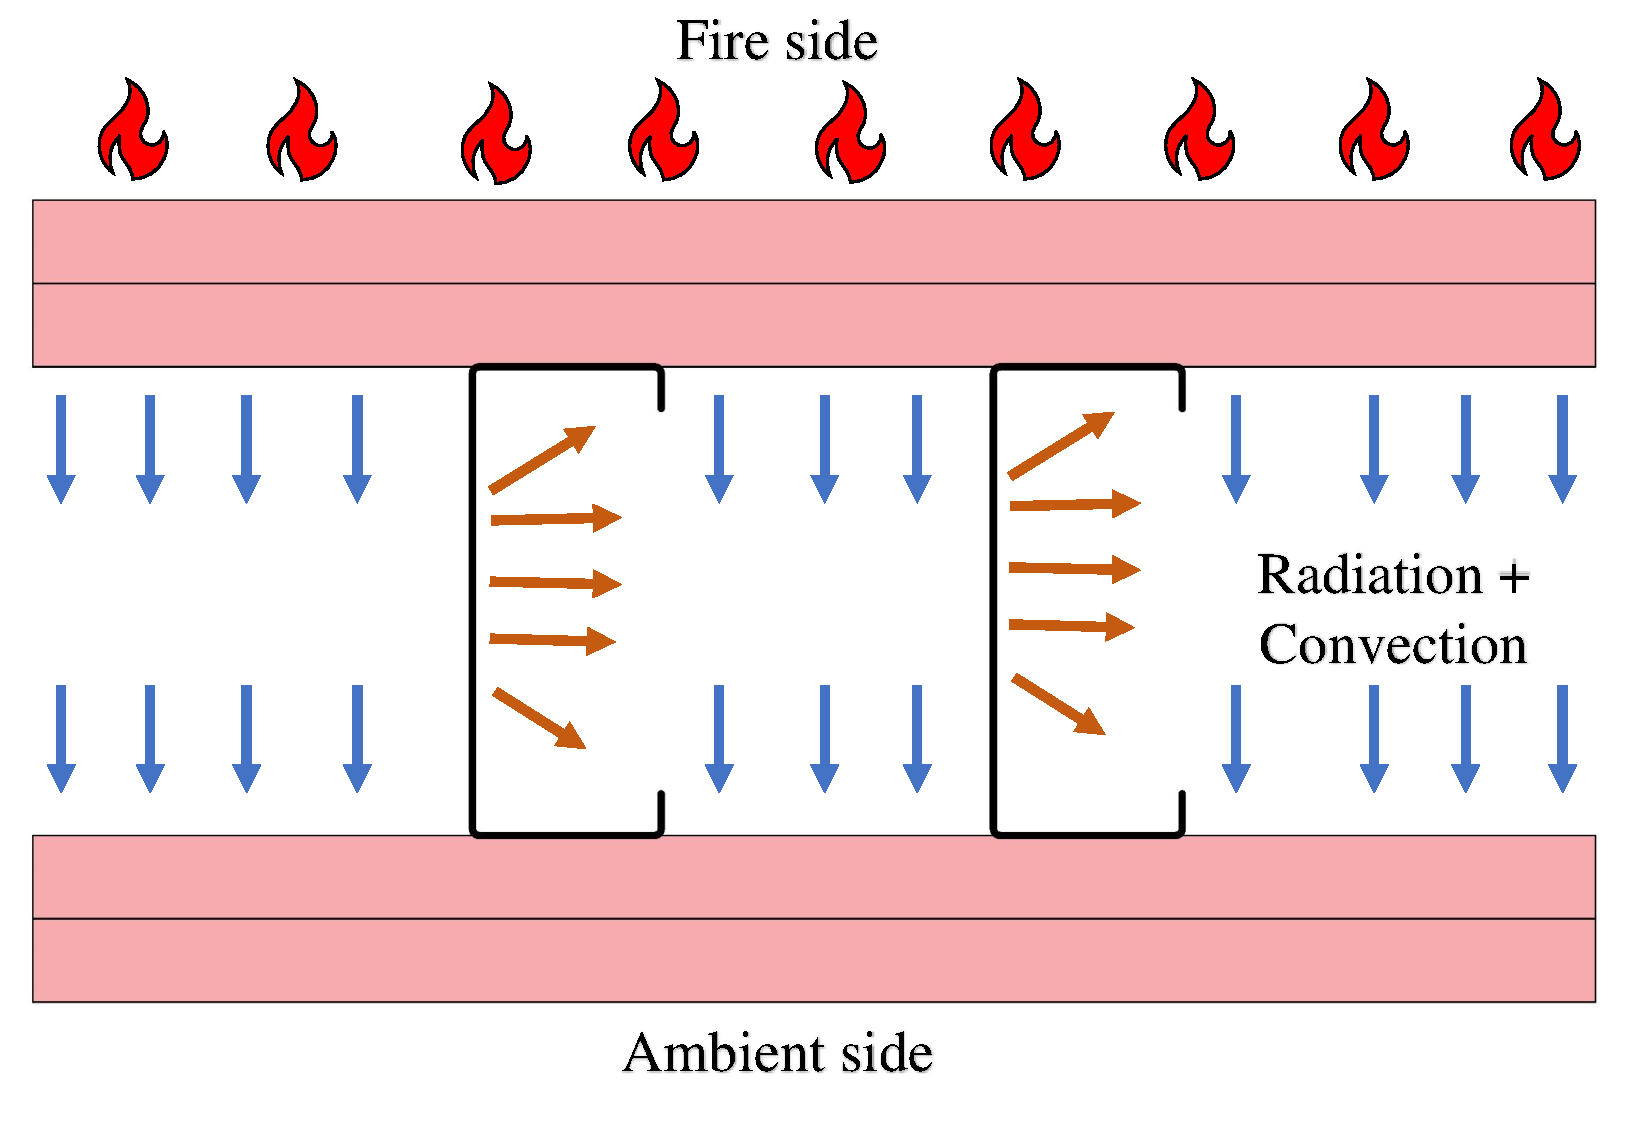
\includegraphics[width=\textwidth]{single-heat-transfer.pdf}
		\caption{}
		\label{subfig:single-heat-transfer}
	\end{subfigure}
	\begin{subfigure}[b]{0.5\textwidth}
		\centering
		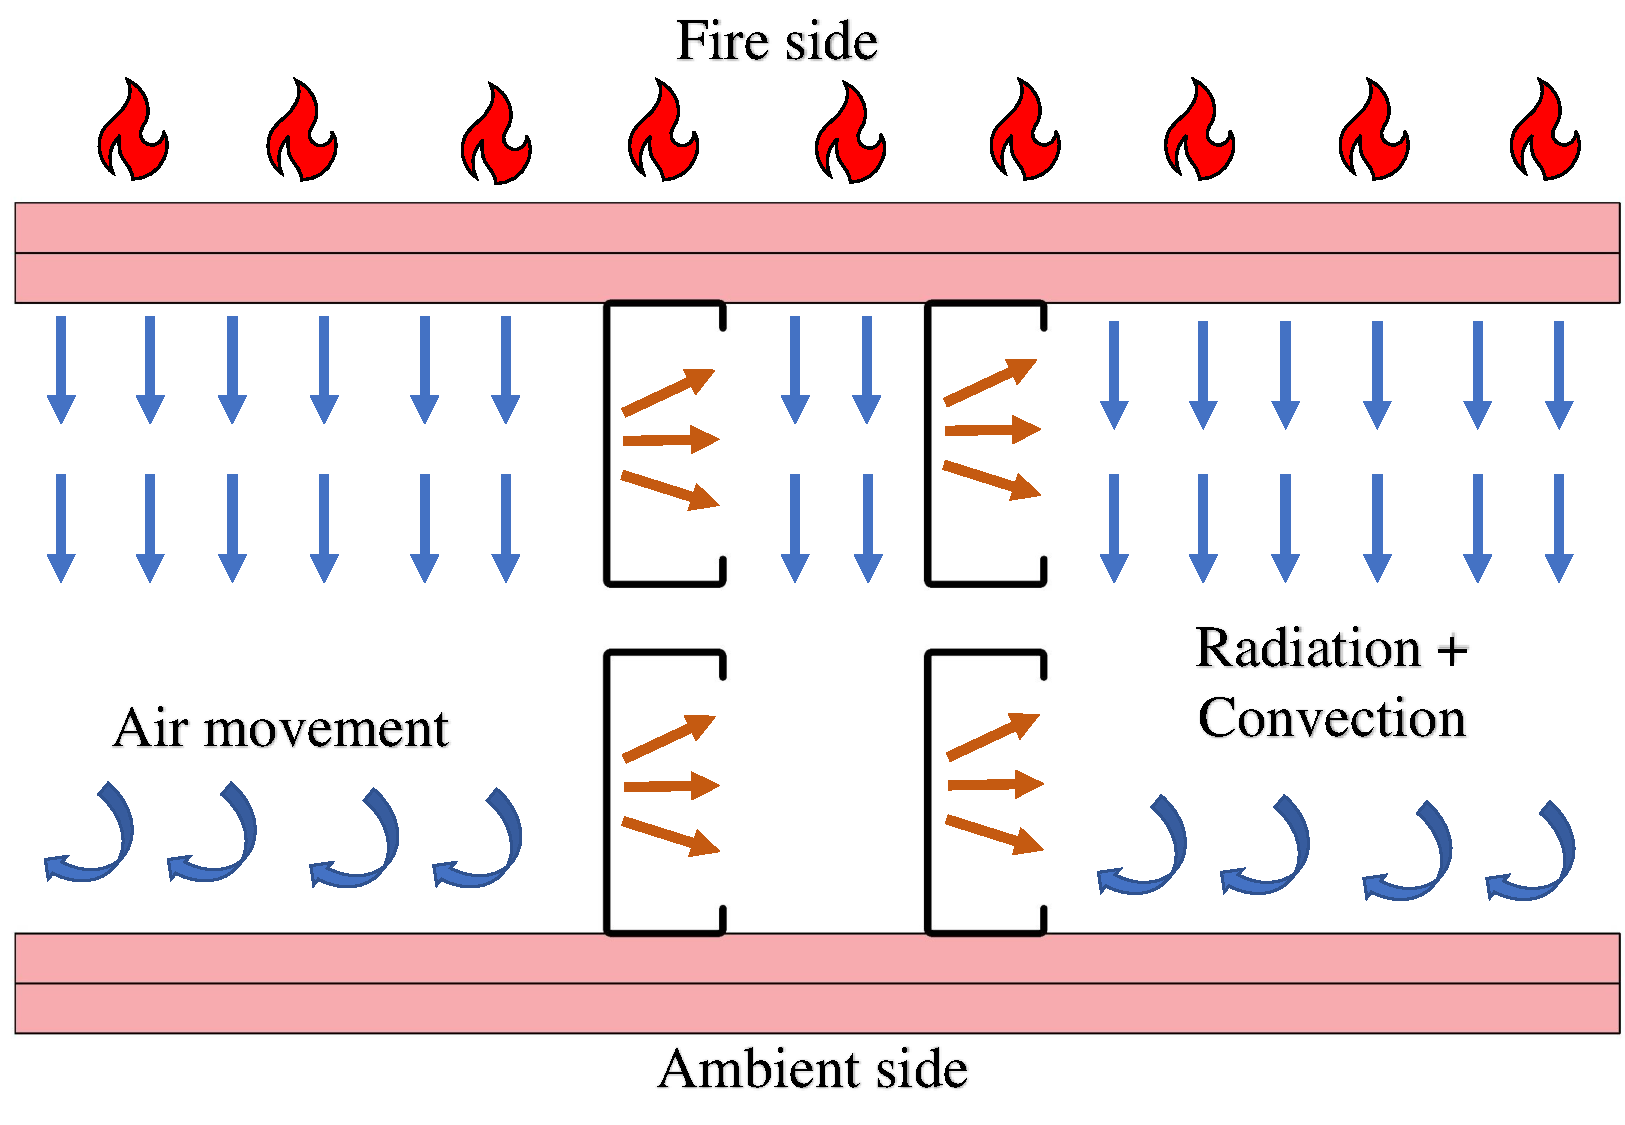
\includegraphics[width=\textwidth]{ds-heat-transfer.pdf}
		\caption{}
		\label{subfig:ds-heat-transfer}
	\end{subfigure}
	   \caption{Heat transfer mechanism in (a) Single stud (b) Double stud LSF walls}
	   \label{fig:heat-transfer}
\end{figure} 

Therefore, to address these issues, a detailed literature review was undertaken and the most suitable thermal models were considered to predict the temperature profiles of the conducted full-scale fire tests in \Cref{ch:Fire}. The developed numerical model was then used to perform thermal analysis on all the conducted full-scale fire tests to predict the time-temperature curves of studs and plasterboards. The predicted time-temperature curves of stud hot and cold flanges will then be used to determine the structural failure times of the complex LSF wall systems and also to validate against the conducted full-scale fire tests. To solve the above-mentioned advanced numerical models it becomes essential to utilize the availability of the computational resources efficiently. 

The advent of high performance computing has helped to address problems of higher order numerical complexity with the advanced processing power. The speed of a computer is determined by the quantum of parallel operations that can be performed in any given time. Computers used for general activities have processing power in a range up to 12 GHz (Giga Hertz), whereas in a high-performance computing facility many nodes will be linked to parent hub forming a cluster. As a result, the processing speed that can be practically achieved can reach up to Tera-Hertz. Finite Element Analysis (FEA) by default uses single point precision memory for solving the numerical analysis as this memory is extracted from the processor in the local node of the computer. Graphical processing unit (GPU) is also called for the analysis in some of the FEA packages (for example ABAQUS), which can then utilize the double point precision memory to solve the numerical problem. Numerical solving time for a problem in the High Performance Computing (HPC) can be exponentially increased by deploying GPU vector parallelization technique. This is generally achieved by clustering the CPU processing cores with the GPU processing cores to minimize the solver time of the FEA package. High-performance computing facility available at the Queensland university of Technology (QUT) was used in this research to solve the thermal numerical models. ABAQUS and FDS thermal models could be natively run in the HPC cluster which operates on Linux operating system. However the source code of SAFIR was modified to make it run in the Linux HPC cluster available at QUT.

\section{Thermal modelling in SAFIR}

SAFIR is a finite element program developed in FORTRAN programming language by the University of Liege to model the behaviour of structures in fire (\citet{safir2017}). Past researchers have extensively used SAFIR to determine the thermal behaviour of LSF walls with various stud sections in fire. This includes research studies of \citet{Keerthan2012a,Keerthan2013} wherein the LSF wall assemblies were modelled in 2D and the thermal analysis were carried out to determine the temperature evolution across the cross-section to simulate the time-temperature curves from full-scale fire tests. Considering the 2D nature of solving the heat transfer problem for computational efficiency, SAFIR was first considered for creating the thermal FE models. GiD, a universal pre and post-processor software, was used to create the model in 2D for this research study. Temperature dependent thermal properties for steel and gypsum plasterboard in LSF walls were extracted from \citet{Maneesha2018}, which were later confirmed by \citet{Steau2020}. Although, the temperature dependant material properties were preloaded in SAFIR for steel and gypsum plasterboard, the apparent thermal properties proposed by \citet{Maneesha2018} (\Cref{fig:plasterboard-thermal,fig:Steel-thermal,fig:Insulation-thermal}) were used in the analysis to better represent the full-scale fire tests. SAFIR solves the heat exchange problem mainly through conduction, which is based on Fourier equation. Firstly, attempt was made to simulate the full-scale fire Test-T1 of a double stud wall from the experimental investigation detailed in \Cref{ch:Fire}. 
\begin{figure}[!htbp]
	\centering
	\begin{subfigure}[b]{0.6\textwidth}
		\centering
		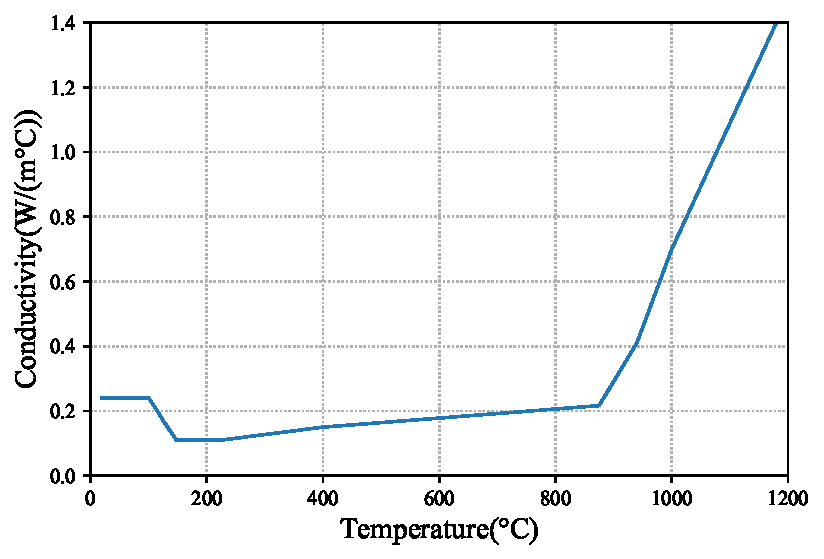
\includegraphics[width=\textwidth]{Plasterboard-conductivity.pdf}
		\caption{}
		\label{subfig:Plasterboard-conductivity}
	\end{subfigure}
	\begin{subfigure}[b]{0.6\textwidth}
		\centering
		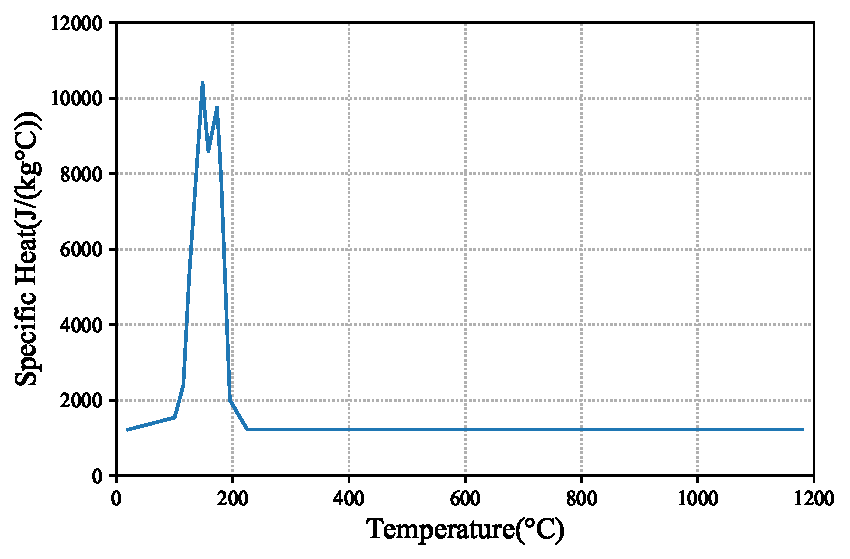
\includegraphics[width=\textwidth]{Plasterboard-specific-heat.pdf}
		\caption{}
		\label{subfig:Plasterboard-specific-heat}
	\end{subfigure}
	   \caption{Elevated temperature thermal properties of plasterboard from \citet{Maneesha2018}}
	   \label{fig:plasterboard-thermal}
\end{figure}
\begin{figure}[!htbp]
	\centering
	\begin{subfigure}[b]{0.6\textwidth}
		\centering
		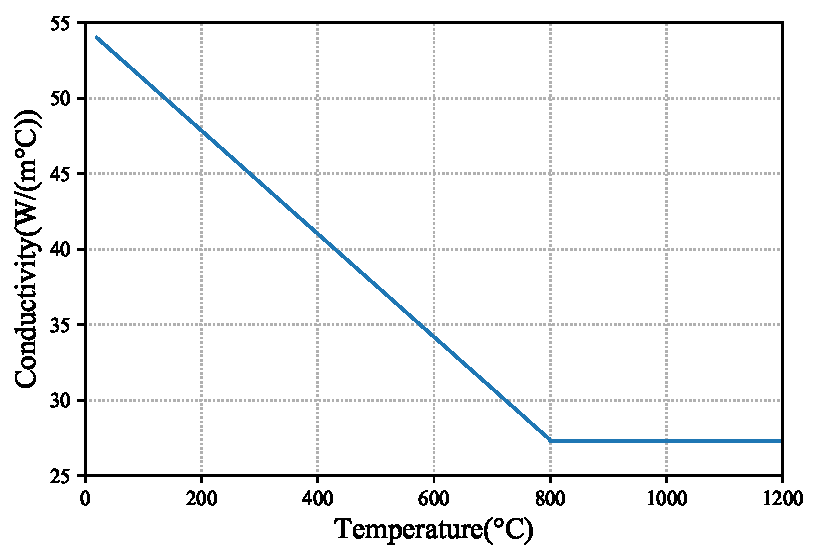
\includegraphics[width=\textwidth]{Steel-conductivity.pdf}
		\caption{}
		\label{subfig:Steel-conductivity}
	\end{subfigure}
	\begin{subfigure}[b]{0.6\textwidth}
		\centering
		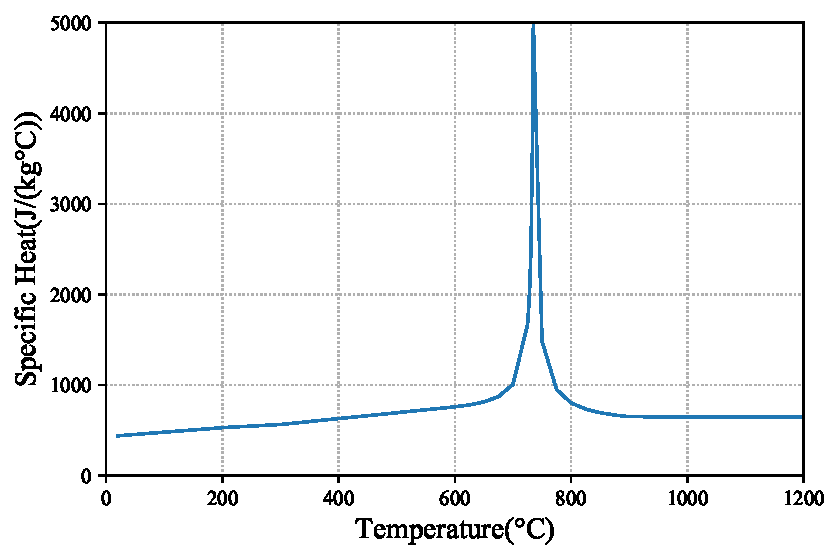
\includegraphics[width=\textwidth]{Steel-specific-heat.pdf}
		\caption{}
		\label{subfig:Steel-specific-heat}
	\end{subfigure}
	   \caption{Elevated temperature thermal properties of steel from \citet{Maneesha2018}}
	   \label{fig:Steel-thermal}
\end{figure}
\begin{figure}[!htbp]
	\centering
	\begin{subfigure}[b]{0.6\textwidth}
		\centering
		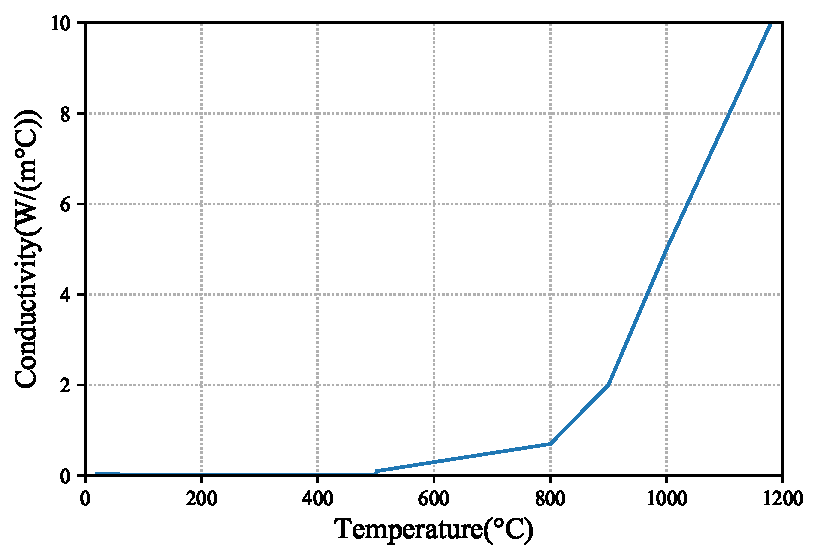
\includegraphics[width=\textwidth]{Insulation-conductivity.pdf}
		\caption{}
		\label{subfig:Insulation-conductivity}
	\end{subfigure}
	   \label{fig:Insulation-thermal-a}
\end{figure}
\begin{figure}[!htbp]
	\ContinuedFloat
	\centering
	\begin{subfigure}[b]{0.6\textwidth}
		\centering
		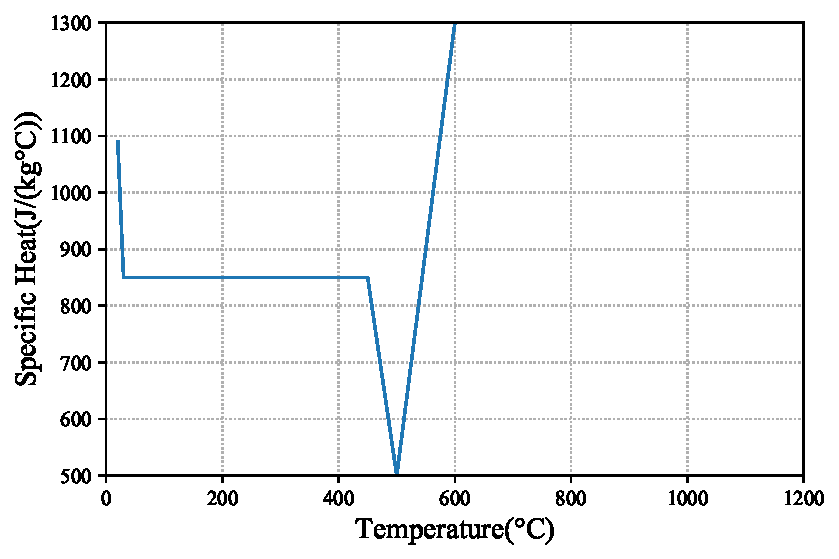
\includegraphics[width=\textwidth]{Insulation-specific-heat.pdf}
		\caption{}
		\label{subfig:Insulation-specific-heat}
	\end{subfigure}
	   \caption{Elevated temperature thermal properties of glass fibre insulation from \citet{Maneesha2018}}
	   \label{fig:Insulation-thermal}
\end{figure}

The 2D model was created with a width of 0.6 m based on past literature (\citet{Keerthan2012a,Keerthan2013}) and the depth of the model was 264 mm representing the overall wall configuration used in Test-T1 (\Cref{fig:safir-model}). Due to symmetry, the models consisted of one set of studs only with 300 mm cavity width on either side of the geometry. Sides of the model were closed with gypsum plasterboard to create a closed cavity. This is because of the limitations in SAFIR to solve models with open cavity. After model creation, Non-uniform rational basis spline (NURB) surfaces were assigned to the 2D model geometry. Frontier conditions were given to the fire and ambient surfaces to specify the ISO 834 standard time-temperature curve on the fire side and ``F20" condition on the ambient side to simulate ambient room temperature condition. No frontier conditions were provided to the side plasterboards to simulate adiabatic conditions, wherein assumption of no heat transfer through the sides was considered. Mesh density was maintained globally at 10 mm throughout the model based on initial sensitivity investigation and from past literature. However, the mesh density is automatically adjusted by the GiD pre-processor near the stud and plasterboard contact as SAFIR allows unstructured meshing for 2D thermal analysis. Triangular meshes were used for the thermal model. \Cref{fig:safir-model} shows the details of the developed double stud model to represent Test-T1 in SAFIR for thermal behaviour prediction. Details about the meshes are shown in \Cref{fig:safir-mesh}
\begin{figure}[!htbp]
	\centering
	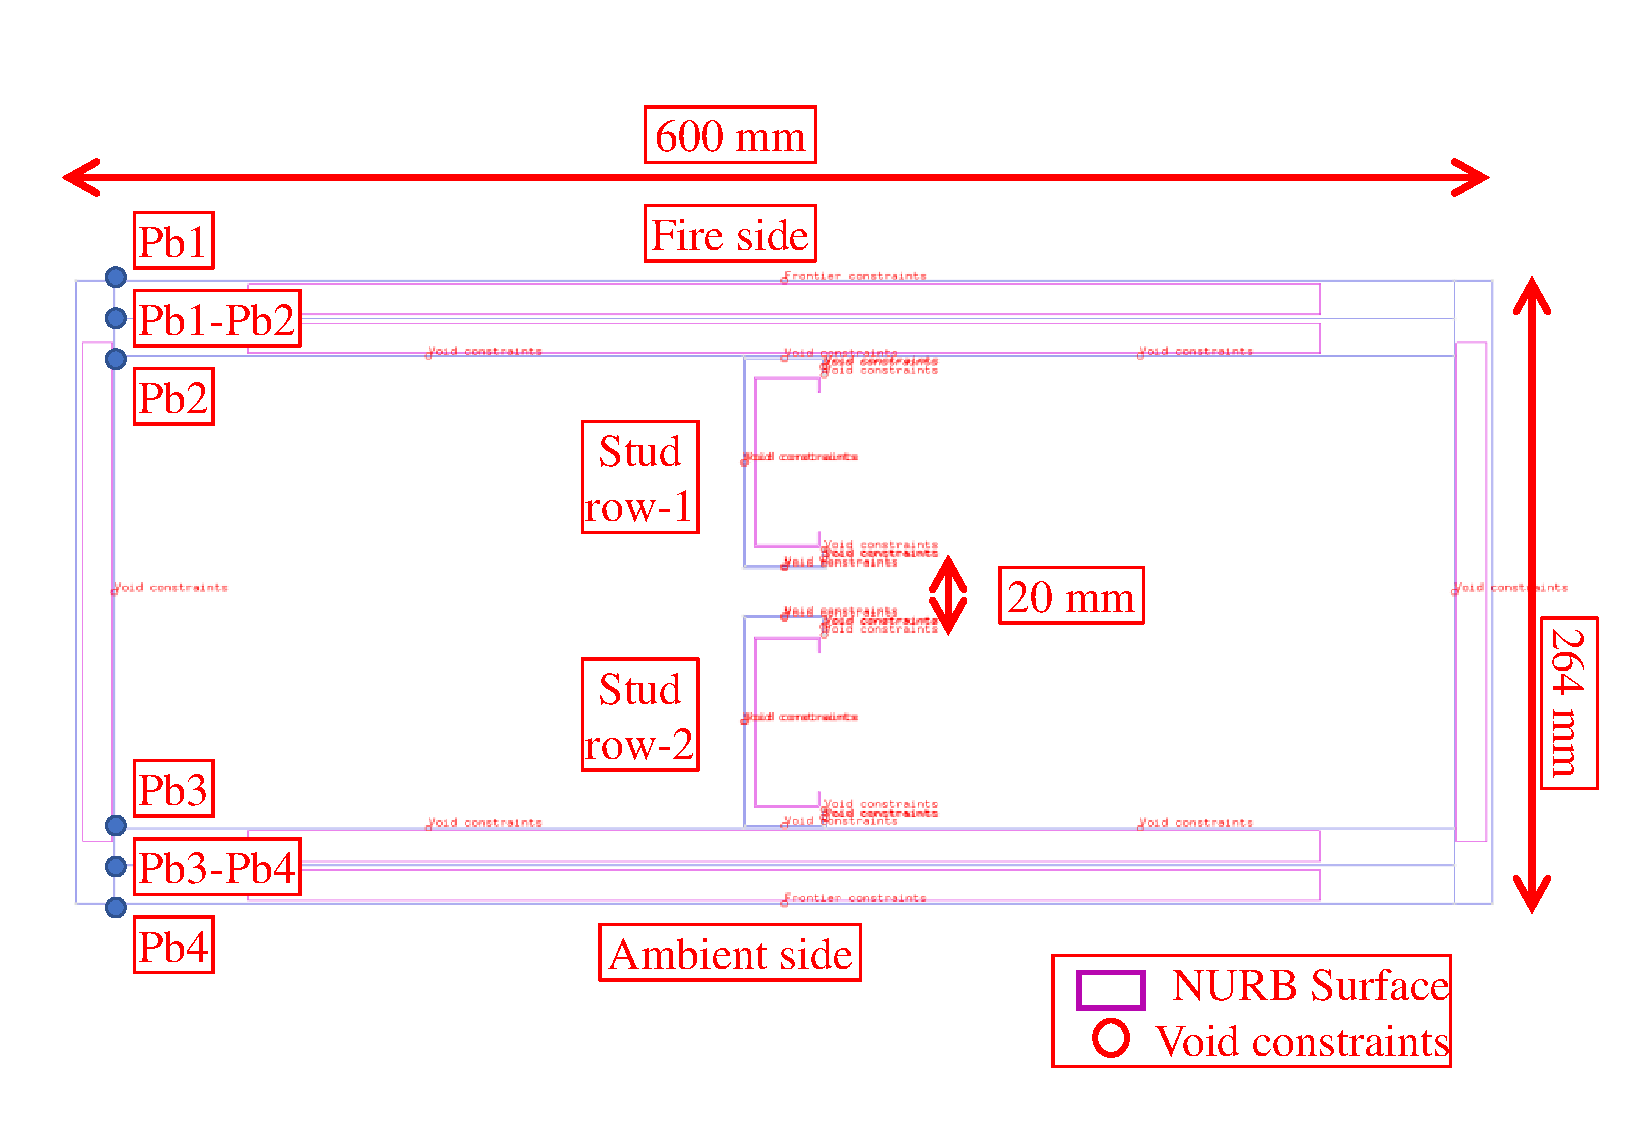
\includegraphics[scale=0.5]{safir-model.pdf}
	\caption{2D model of Test-T1 in SAFIR using GiD interface}
	\label{fig:safir-model}
	% \fontsize{10}{1}\textit{Note : All dimensions are in mm.}
\end{figure}
\begin{figure}[!htbp]
	\centering
	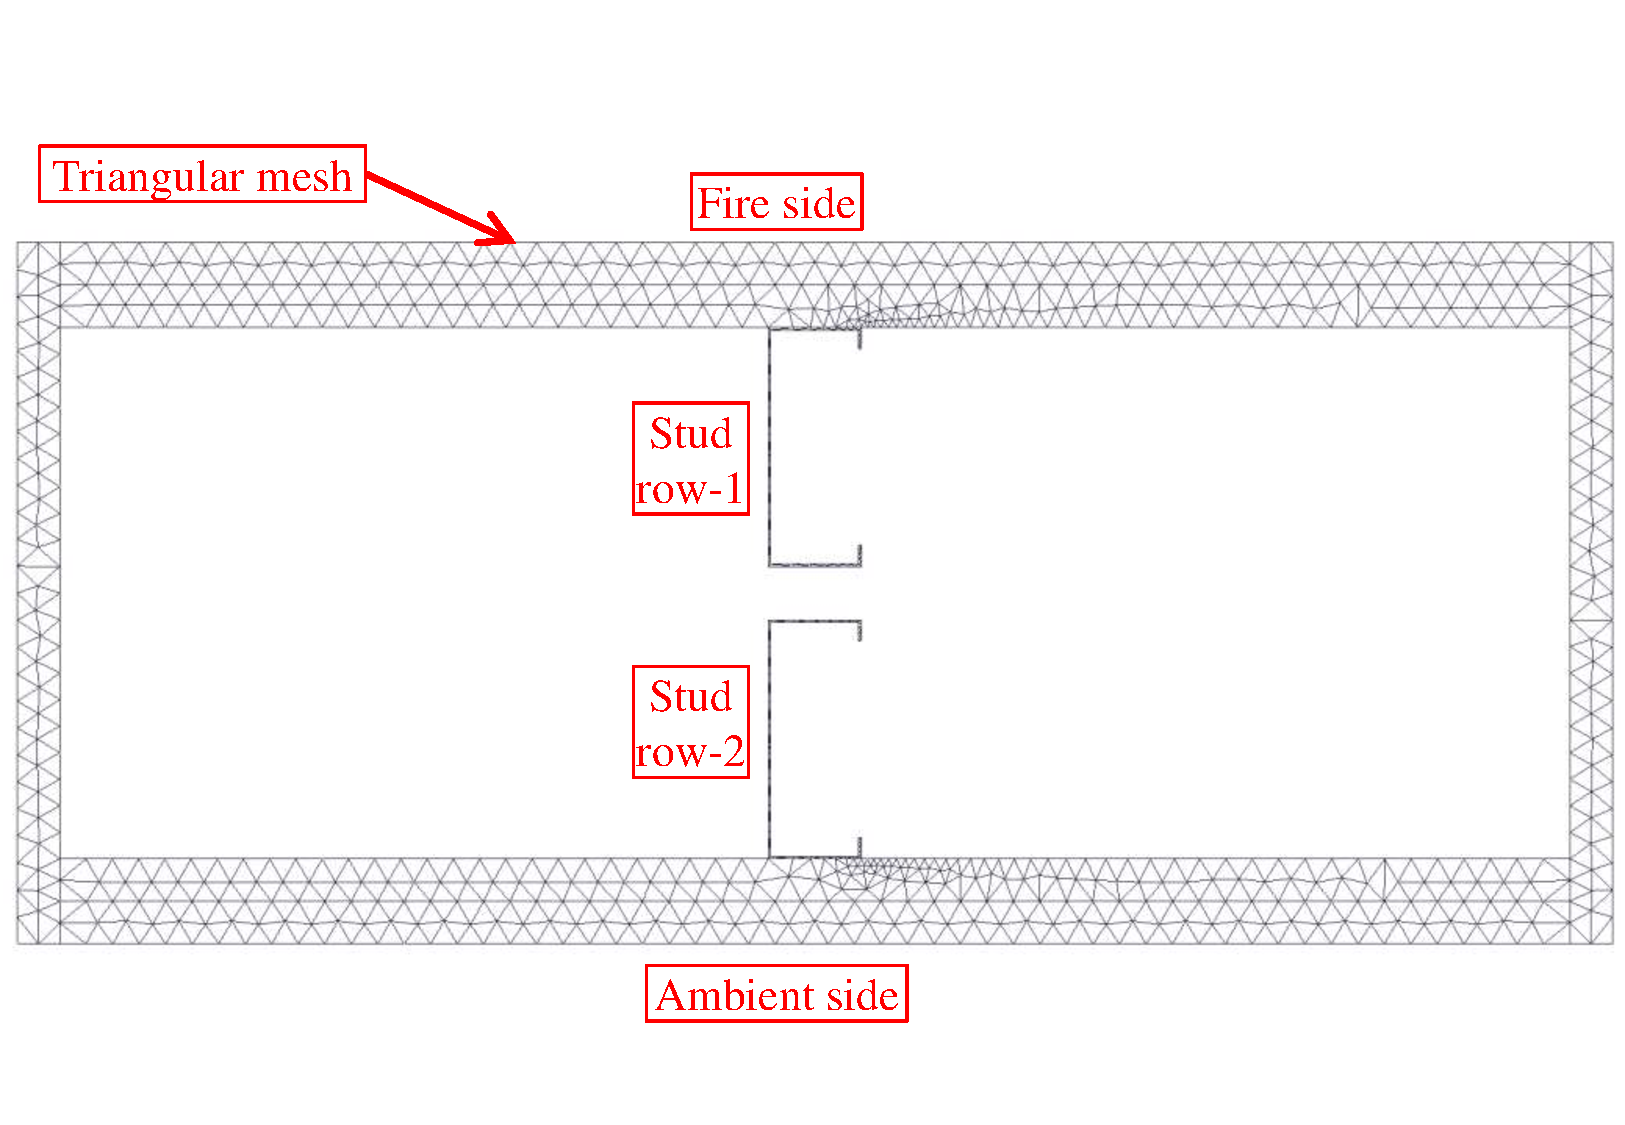
\includegraphics[scale=0.45]{safir-mesh.pdf}
	\caption{2D model mesh of Test-T1 in SAFIR using GiD interface}
	\label{fig:safir-mesh}
\end{figure}

The thermal properties were applied to the corresponding surfaces through the input file as GiD-SAFIR interface does not have the ability to assign multiple user defined material properties through graphical input methods. Convective heat transfer coefficient of 25 W/m$^2$\degree C was assigned to the fire side while 10 W/m$^2$\degree C was assigned the ambient side plasterboard surface. Relative emissivity of 0.9 was specified to the cavity. ISO 834 standard time-temperature curve was used as the fire side boundary condition and was preloaded in the SAFIR package. The boundary condition on the ambient side was assigned to be at room temperatures by using the ``F20 Frontier condition". The sides of the model were assumed to be adiabatic. All the models were analysed for a time period of 240 min. The thermal analysis results were post-processed with the help of DIAMOND, a software package specifically designed to view and post process SAFIR analysis results. Thermal analysis output from the models are shown in \Cref{fig:safir-output,fig:safir-output-studs}.
\begin{figure}[!htbp]
	\centering
	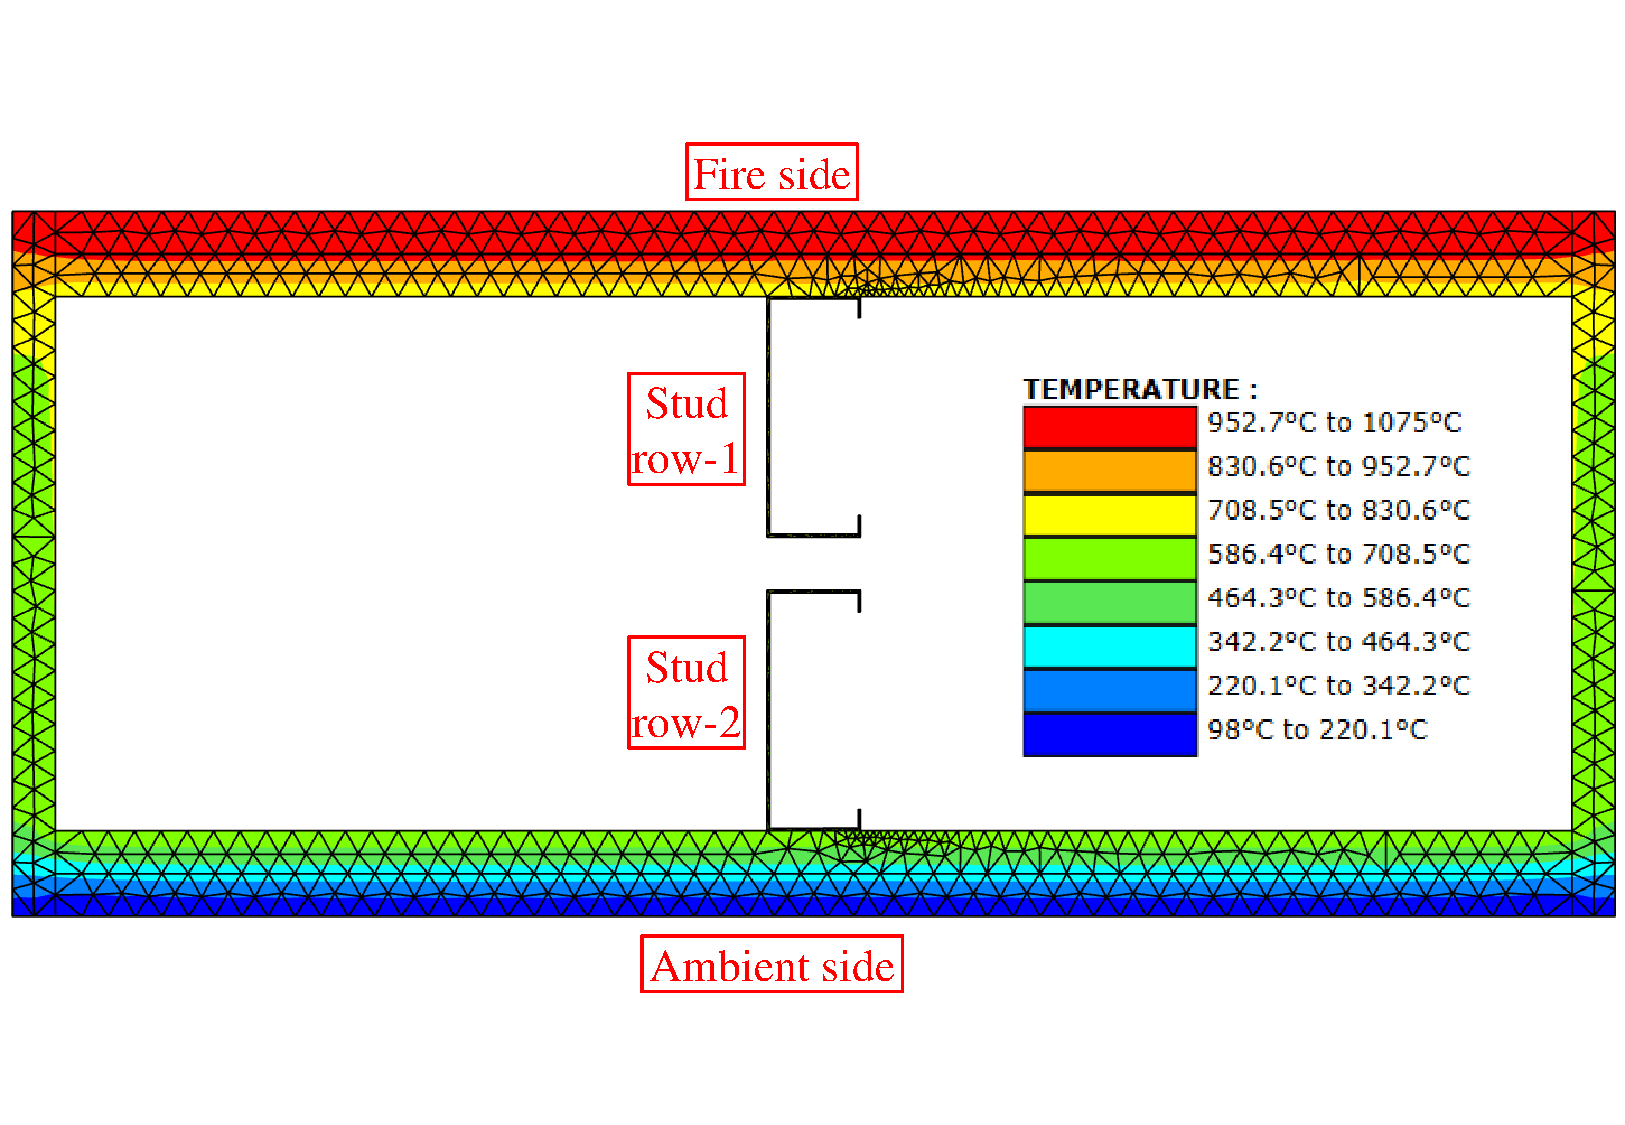
\includegraphics[scale=0.5]{safir-output.pdf}
	\caption{Thermal analysis output from SAFIR 2D model}
	\label{fig:safir-output}
\end{figure}
\begin{figure}[!htbp]
	\centering
	\begin{subfigure}[b]{0.4\textwidth}
		\centering
		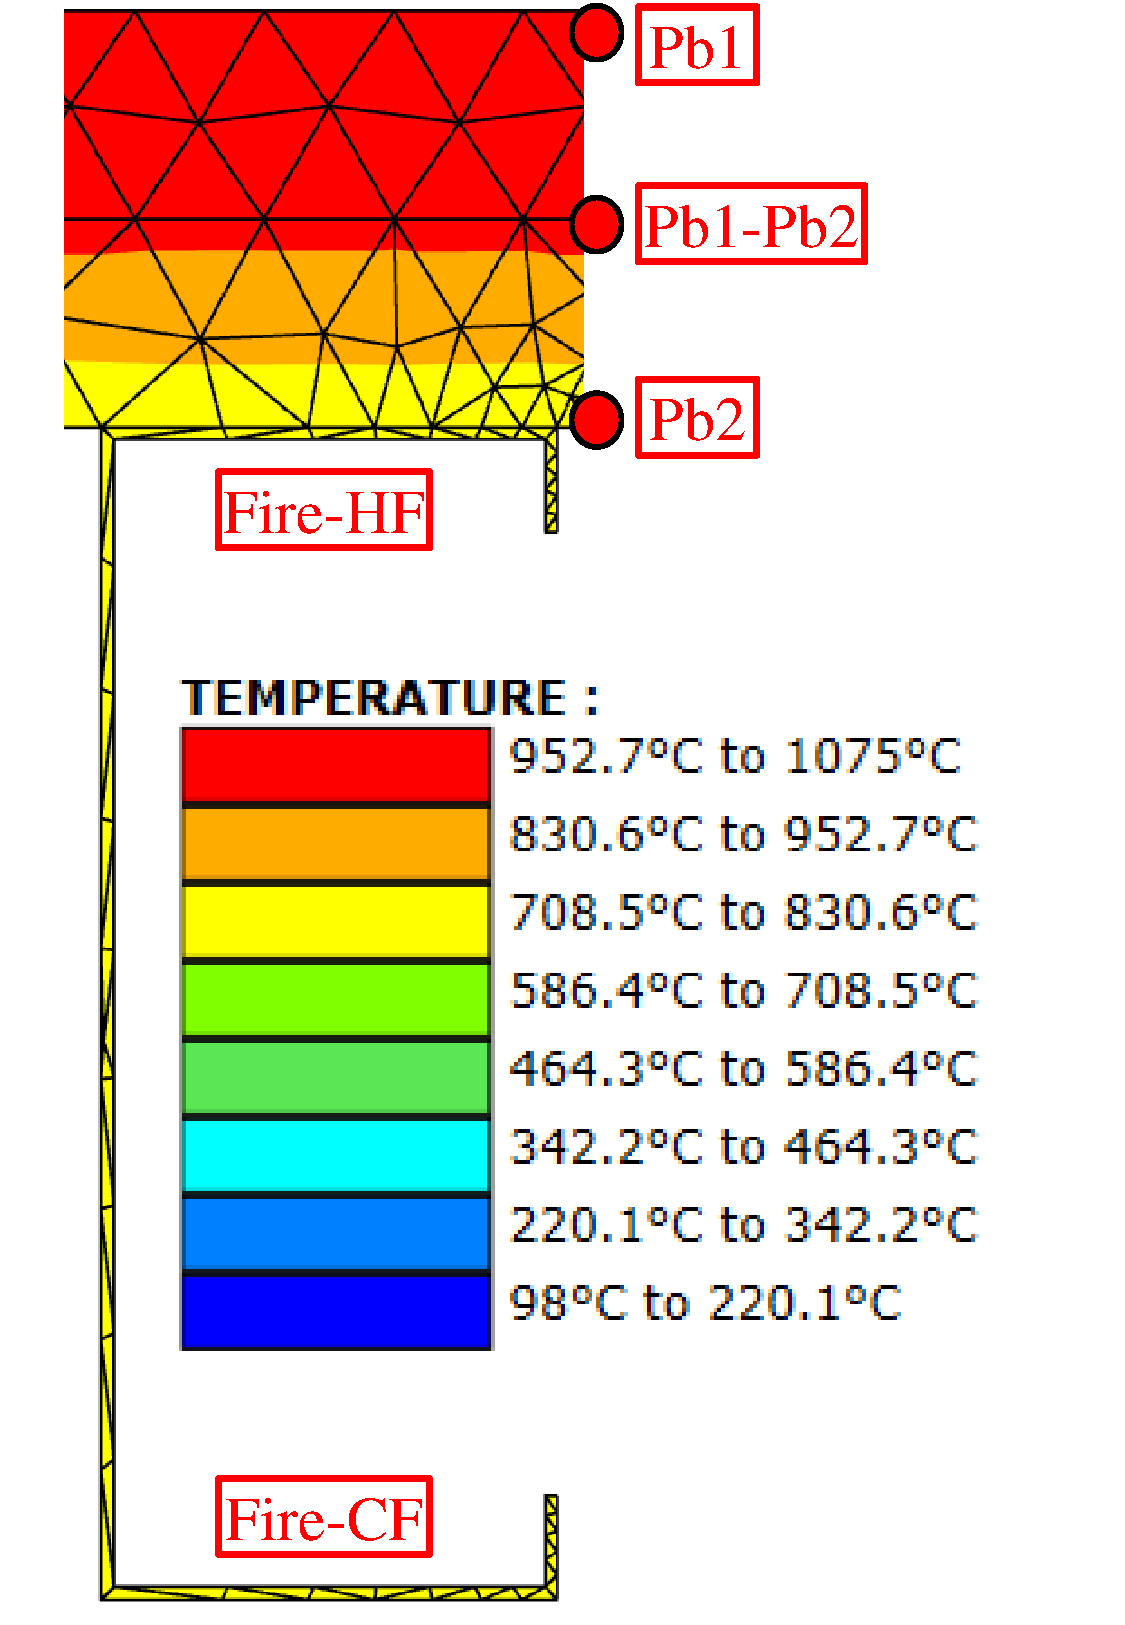
\includegraphics[width=\textwidth]{safir-output-fhf.pdf}
		\caption{}
		\label{subfig:safir-output-fhf}
	\end{subfigure}
	\begin{subfigure}[b]{0.4\textwidth}
		\centering
		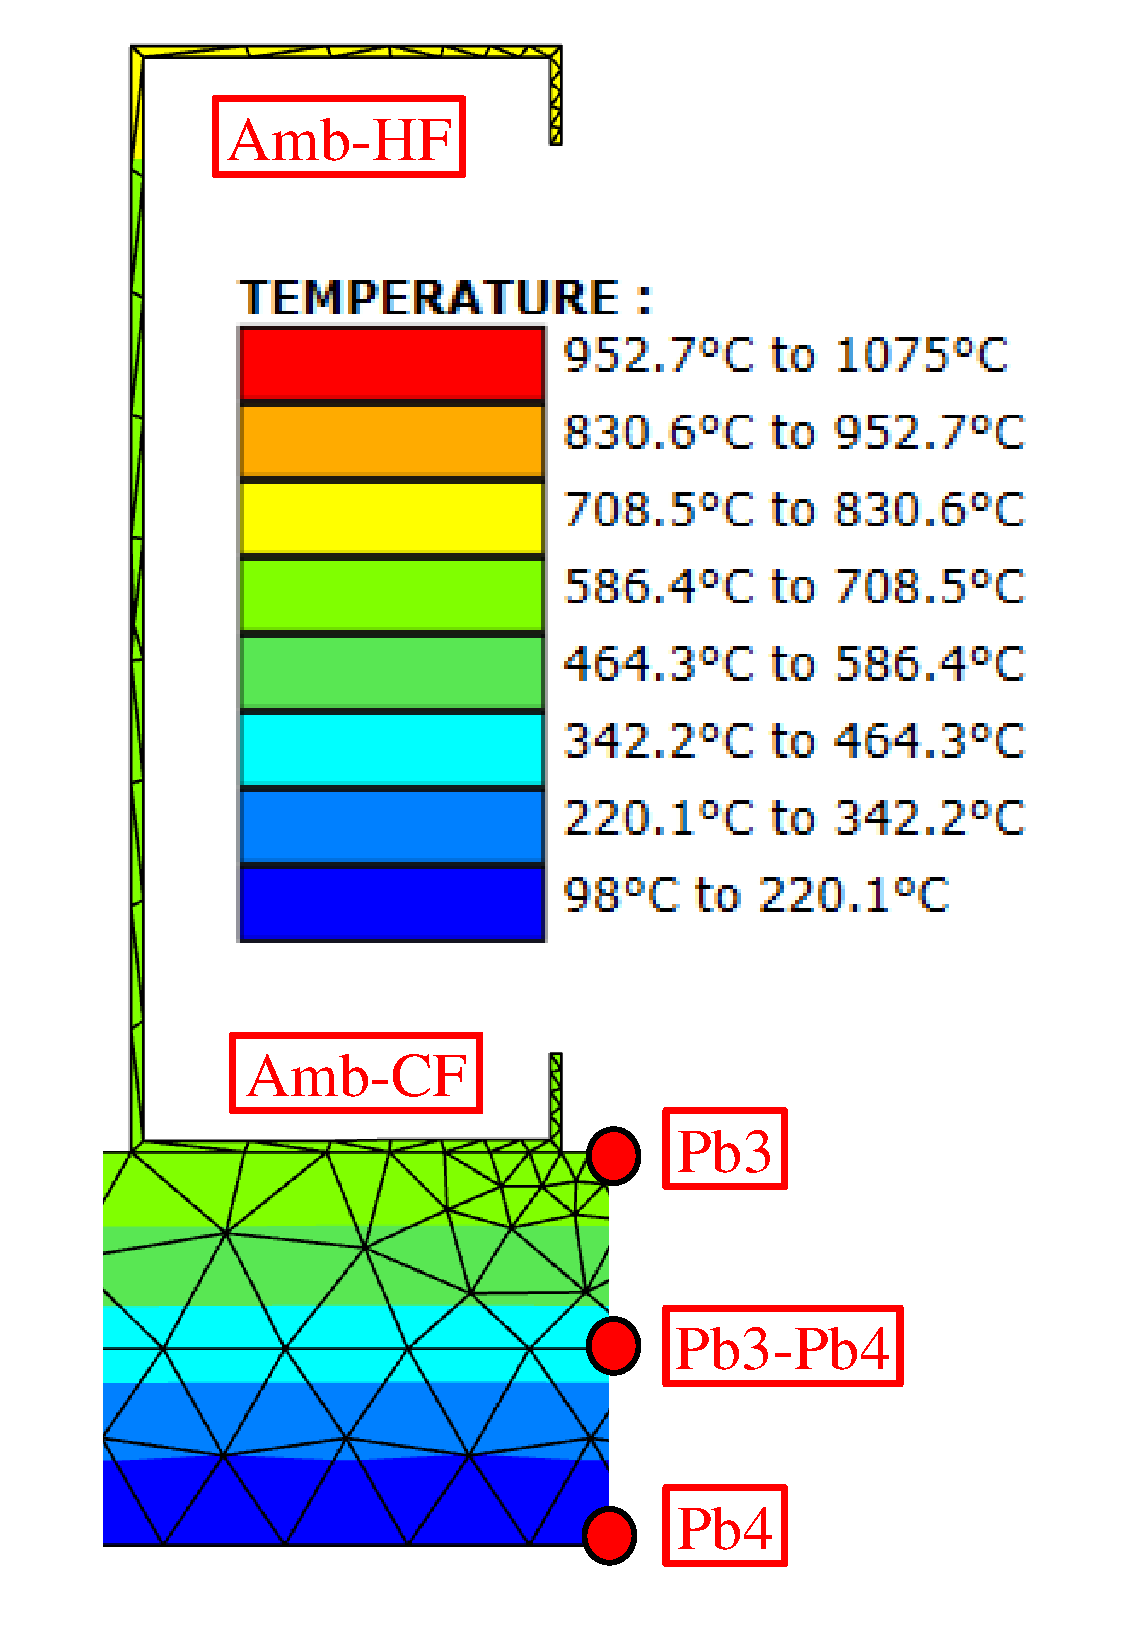
\includegraphics[width=\textwidth]{safir-output-ahf.pdf}
		\caption{}
		\label{subfig:safir-output-ahf}
	\end{subfigure}
	   \caption{Thermal analysis output of studs from SAFIR 2D model (a) Fire side stud (b) Ambient side stud}
	   \label{fig:safir-output-studs}
\end{figure}

Some general notations will be followed throughout this paper, to easily identify the surfaces on which thermocouple measurements were taken and considered for comparison as shown in \Cref{fig:safir-output-studs,fig:T1-safir-vs-experiment}. Pb1 and Pb4 refer to the fire side and the ambient side plasterboard surfaces. Fire side and ambient side plasterboard cavity surfaces are referred to as Pb2 and Pb3. The interface between the two plasterboard layers on the fire side is referred to as Pb1-Pb2 while the interface between the ambient side plasterboards is referred to as Pb3-Pb4 for all fire tests except Test-T4. The hot and cold flanges of single stud walls are referred to as HF and CF. Also, the average plasterboard time-temperature curves from the experiments will be used for the comparison against the thermal model predictions. This is because of the large surface area of the specimen in the full-scale fire test resulting in different temperatures along the height of the test wall. However, the stud time-temperature curves measured at mid-height of the test wall (1500 mm) will be considered for comparison as the surface area of the studs is low in comparison with the plasterboards. The mid-height thermocouple is selected instead of average thermocouple measurements along the height because the temperature measurements at the top will be hotter and at the bottom will be cooler. Computing the average would not be ideal for comparison due to the higher temperature gradient along the stud height. \Cref{subfig:T1-r4-Plasterboard-Safir-vs-Exp} shows the plasterboard time-temperature curves from SAFIR thermal analysis compared against experimental results. The fire side plasterboard temperatures (Pb1) shows good agreement in comparison with the experimental results. It is to be noted that the Pb1 time-temperature curve is given as the fire side ``Frontier condition" to the thermal model to better simulate the experiments. The fire side plasterboard interface time-temperature curve exhibited a plateau region in the experiments. This behaviour is attributed to various factors such as increased convection, moisture transfer. However, simulating these effects are challenging and is beyond the scope of this study. The Pb1-Pb2 time-temperature curve from SAFIR thermal analysis exhibited reasonable agreement with the experimental results till 60 min after which the predictions from SAFIR were higher. Likewise, the fire side cavity (Pb2) and the ambient side cavity (Pb3) time-temperature curves agreed well with the experimental results till 60 and 80 min, respectively, after which a steep increase in the time-temperature curve is observed. This results in increased time-temperature curve on the ambient side plasterboard interface (Pb3-Pb4) and the ambient side plasterboard surface (Pb4). 
\begin{figure}[!htbp]
	\centering
	\begin{subfigure}[b]{0.7\textwidth}
		\centering
		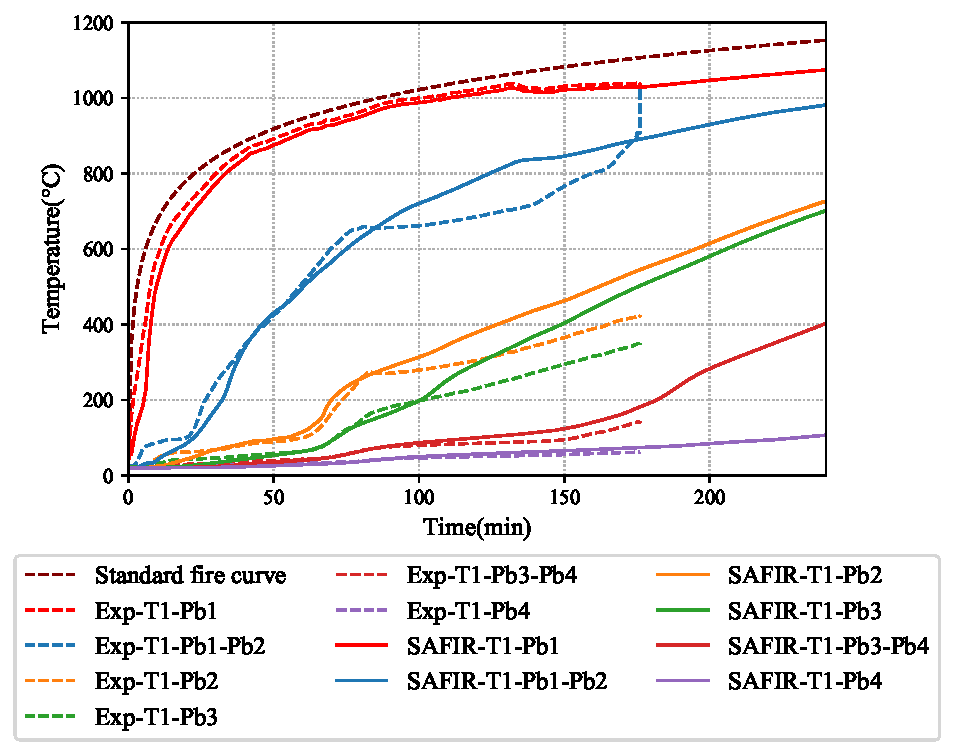
\includegraphics[width=\textwidth]{T1-r4-Plasterboard-Safir-vs-Exp.pdf}
		\caption{}
		\label{subfig:T1-r4-Plasterboard-Safir-vs-Exp}
	\end{subfigure}
	\begin{subfigure}[b]{0.6\textwidth}
		\centering
		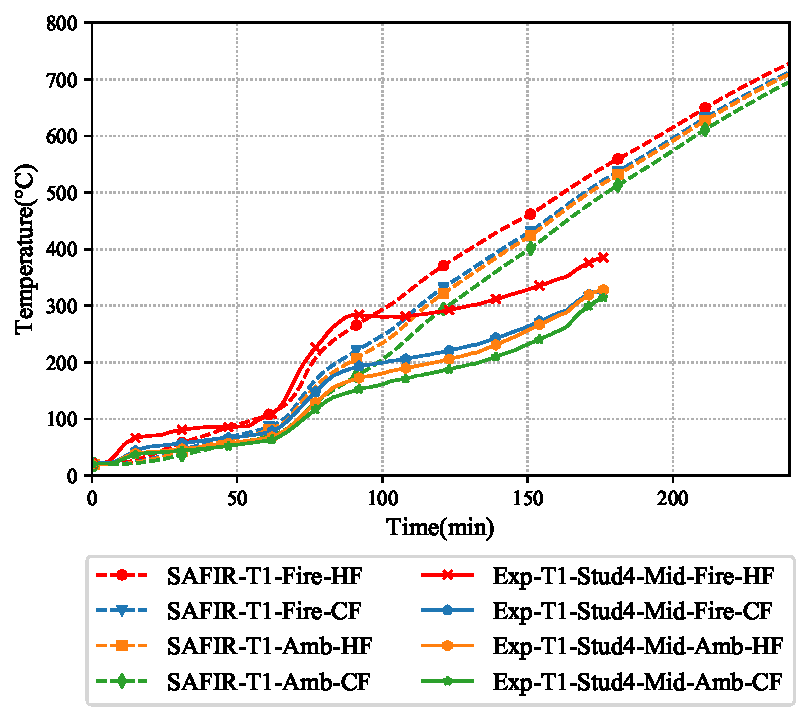
\includegraphics[width=\textwidth]{T1-r4-Studs-4-Safir-vs-Exp.pdf}
		\caption{}
		\label{subfig:T1-r4-Studs-4-Safir-vs-Exp}
	\end{subfigure}
	   \caption{Comparison of the time temperature curves from SAFIR thermal analysis and experiments (a) Average plasterboard temperatures (b) Stud4-Mid temperatures}
	   \label{fig:T1-safir-vs-experiment}
\end{figure}

\Cref{subfig:T1-r4-Plasterboard-Safir-vs-Exp} compares the time-temperature curves of the studs. The stud time-temperature curves of all the hot and cold flanges agreed reasonably well till 60 min in comparison with the experimental results. However, the predictions after 60 min from SAFIR thermal analysis were higher in comparison with the experimental results. The maximum temperature recorded by T1-Stud4-Fire-HF was 385\degree C at 176 min while the Fire-HF temperature predicted by SAFIR was 544\degree C at 176 min. The temperature of the corresponding cold flange from the experiment was 329\degree C while it was 521\degree C from SAFIR thermal model. The ambient side hot and cold flange temperature predictions were also high from the SAFIR thermal model in comparison with the experimental results. It is to be noted that the difference in temperatures between the hot and cold flanges were minimal in the thermal model predictions. This results in over estimation of the time-temperature curve predictions in comparison with the experiments. The presence of wider cavity in double stud LSF walls (200 mm) in comparison with conventional single stud LSF wall with 90 mm cavity might have attributed to this reduced temperature profile. The discontinuous stud arrangement in double stud LSF wall fire Test-T1 along with the wider cavity was identified as the prime reason for the reduced time-temperature curves on the studs and these effects could not be predicted by the SAFIR thermal model. The effect of convection is also higher due to the wider cavity in complex LSF walls and this effect has to be accounted in the thermal model. SAFIR solves the conduction problem for a cartesian system of coordinates based on Fourier equation as shown in \Cref{eq:safir-conduction}.
\begin{equation}\label{eq:safir-conduction}
	\dfrac{\partial}{\partial_x}\left(k\dfrac{\partial T}{\partial_x}\right)+\dfrac{\partial}{\partial_y}\left(k\dfrac{\partial T}{\partial_y}\right)+\dfrac{\partial}{\partial_z}\left(k\dfrac{\partial T}{\partial_z}\right)+Q=c\rho\dfrac{\partial T}{\partial t}
\end{equation}
Where,
\begin{description}[itemsep=0pt,parsep=0pt]
	\item $x,y,x$ = vector of cartesian coordinates (m),
	\item $T$ = temperature (K),
	\item $k$ = thermal conductivity (W/mK),
	\item $Q$ = term to account for internal generation of heat (W/m$^3$),
	\item $\rho$ = specific mass (kg/m$^3$)
	\item $c$ = specific heat(J/kgK),
	\item $t$ = time (s).
\end{description}

Heat exchange on the surfaces and internal cavities is based on linear convection shown in \Cref{eq:safir-convection}. The law of grey bodies is used for radiative flux calculations as shown in \Cref{eq:safir-radiation}
\begin{equation}\label{eq:safir-convection}
	h_c = h\left(T_g - T_s\right)
\end{equation}
Where,
\begin{description}[itemsep=0pt,parsep=0pt]
	\item $h_c$ = convective heat flux between solid and gas (W/m$^2$),
	\item $h$ = coefficient of convection (W/m$^2$K),
	\item $T_g$ = temperature of gas (K),
	\item $T_s$ = temperature of solid surface (K).
\end{description}
\begin{equation}\label{eq:safir-radiation}
	h_r = h\left(T_g - T_s\right)
\end{equation}
Where,
\begin{description}[itemsep=0pt,parsep=0pt]
	\item $h_c$ = convective heat flux between solid and gas (W/m$^2$),
	\item $h$ = coefficient of convection (W/m$^2$K),
	\item $T_g$ = temperature of gas (K),
	\item $T_s$ = temperature of solid surface (K).
\end{description}

As mentioned in \Cref{eq:safir-convection} the effect of convection is linearized within the cavity in SAFIR heat transfer calculations. Simulating the effect of natural convection by approximation within the cavity is not well documented in SAFIR and hence could not be used in the developed model to predict these effects resulting in higher temperature predictions in the studs. As the failure time of the test wall is based on the critical hot flange temperature, the temperature predictions of the stud hot flanges from SAFIR will result in premature structural failure time predictions in comparison with the test wall. Therefore, it becomes a necessity to develop a thermal model to accurately predict the temperature evolution of studs in complex LSF wall systems under fire. Considering the above-mentioned limitations in SAFIR with respect to predicting the time-temperature curves of complex LSF walls exposed to standard fire curve, investigations were then conducted using the most commonly used FEA package ABAQUS and the corresponding discussions are shown next.

\section{Thermal modelling in ABAQUS}

ABAQUS is one of the commonly used FE packages to solve structural and heat transfer problems. Three-dimensional heat transfer brick element (DC3D8) was used to create the plasterboard and studs for the FE thermal model. SI units were followed in model creation wherein the studs and plasterboards were modelled in 3D. The model was 1200 mm wide and 600 mm high considering the symmetry of LSF wall based on past research conducted by \citet{Rusthi2017,Ariyanayagam2019}. Mesh density was kept at 10 mm throughout the studs and 20 mm along the length of the wall for plasterboards. Across the width of the wall near the plasterboards, a mesh density of 4 mm was adopted based on past research and sensitivity analysis. \Cref{fig:abaqus-typical-model-thermal,fig:abaqus-typical-mesh-thermal} show typical model and mesh details used for thermal analysis in ABAQUS. Temperature dependent thermal properties based on past research from \citet{Maneesha2018} were used in the analysis. The FE model for thermal analysis consisted of one stud only connected to the plasterboards at the centre. Cavity width of 300 mm was maintained on both sides of the studs. The cavity was closed on the top and bottom in the model for the thermal analysis as simulating open cavity with symmetry boundary conditions results in extensive computational cost. Tie conditions were provided as constraints on the interface between the stud flanges and the plasterboard surfaces facing the cavity. Radiation was assumed to be predominant within the cavity. An emissivity of 0.9 was specified within the cavity. Convection and radiation boundary conditions were given to the fire and ambient side surfaces. Convective heat transfer coefficient of 25 W/m$^2$\degree C was applied to the fire side while 10 W/m$^2$\degree C was specified on the ambient side plasterboard surface. The tracks and noggings were not considered in the thermal analysis as the effect on the thermal behaviour was insignificant. ISO 834 Standard fire curve was specified as the input boundary condition to the thermal model. Thermal analysis was carried out for a time period of 240 min to simulate the thermal behaviour of double stud wall Test-T1.
\begin{figure}[!htbp]
	\centering
		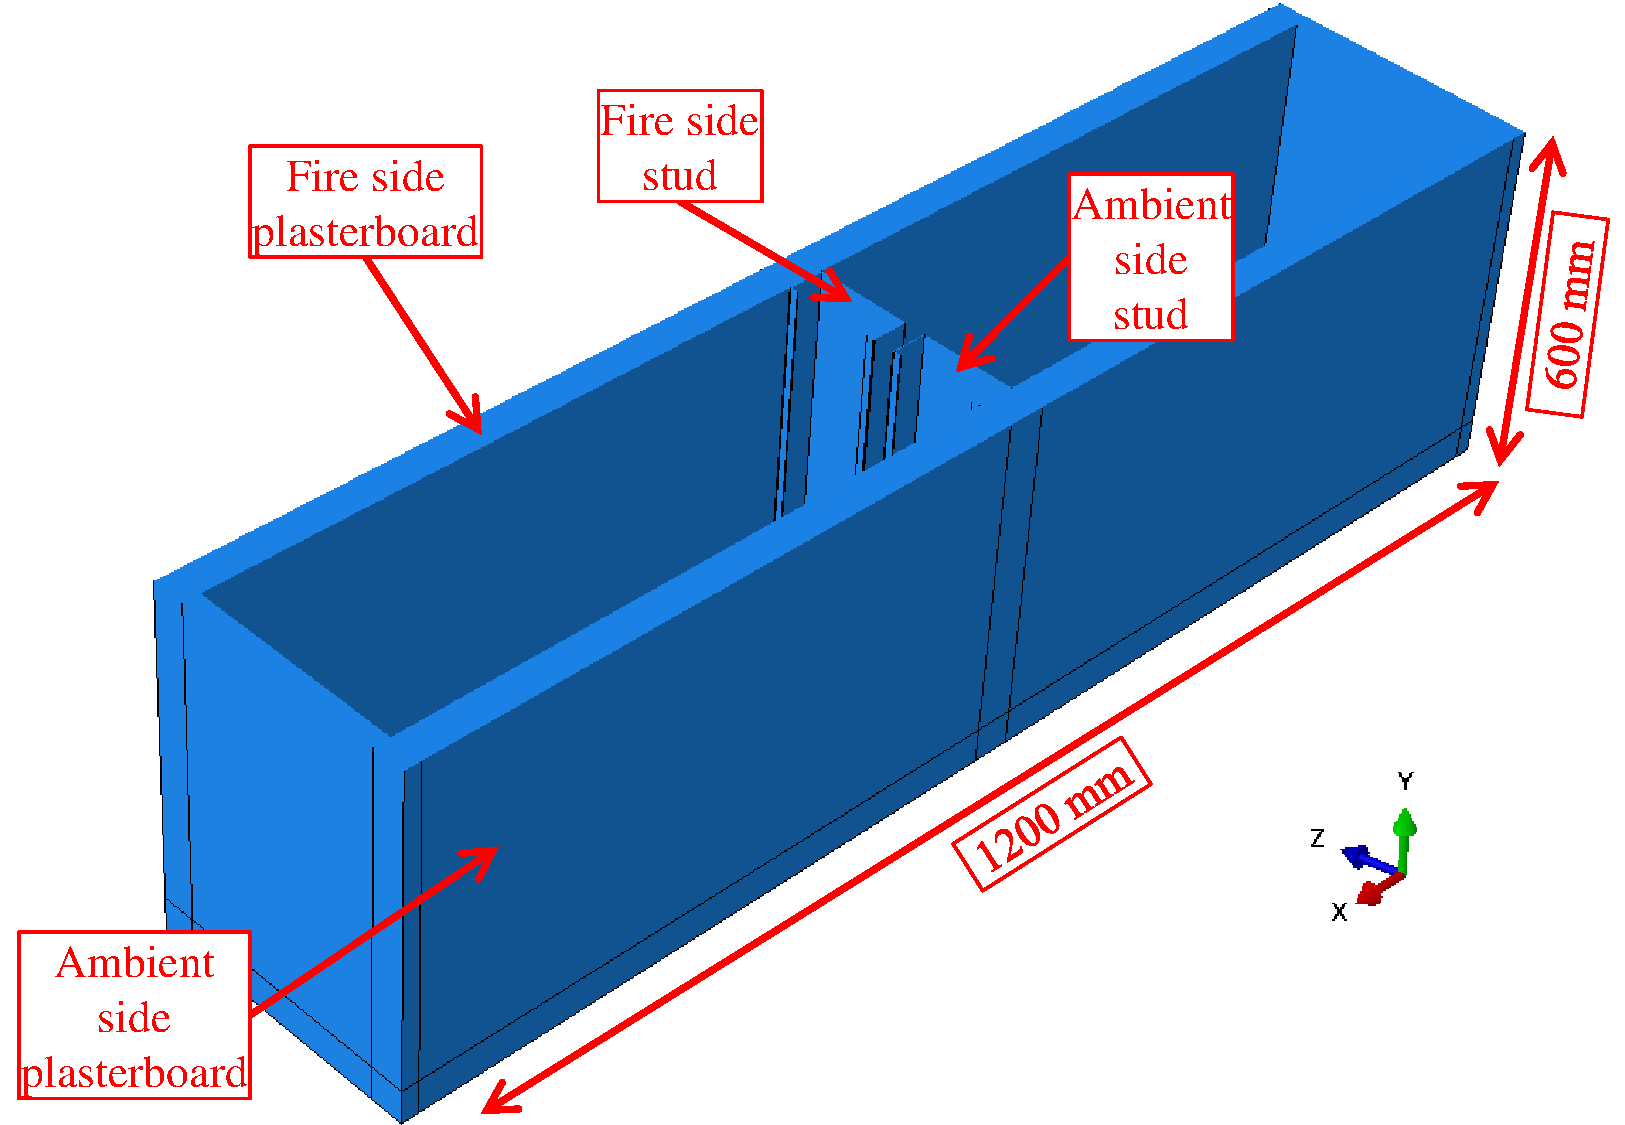
\includegraphics[scale=0.4]{abaqus-typical-model.pdf}
		\caption{3D model of double stud wall in ABAQUS}
		\label{fig:abaqus-typical-model-thermal}
\end{figure}
\begin{figure}[!htbp]
	\centering
		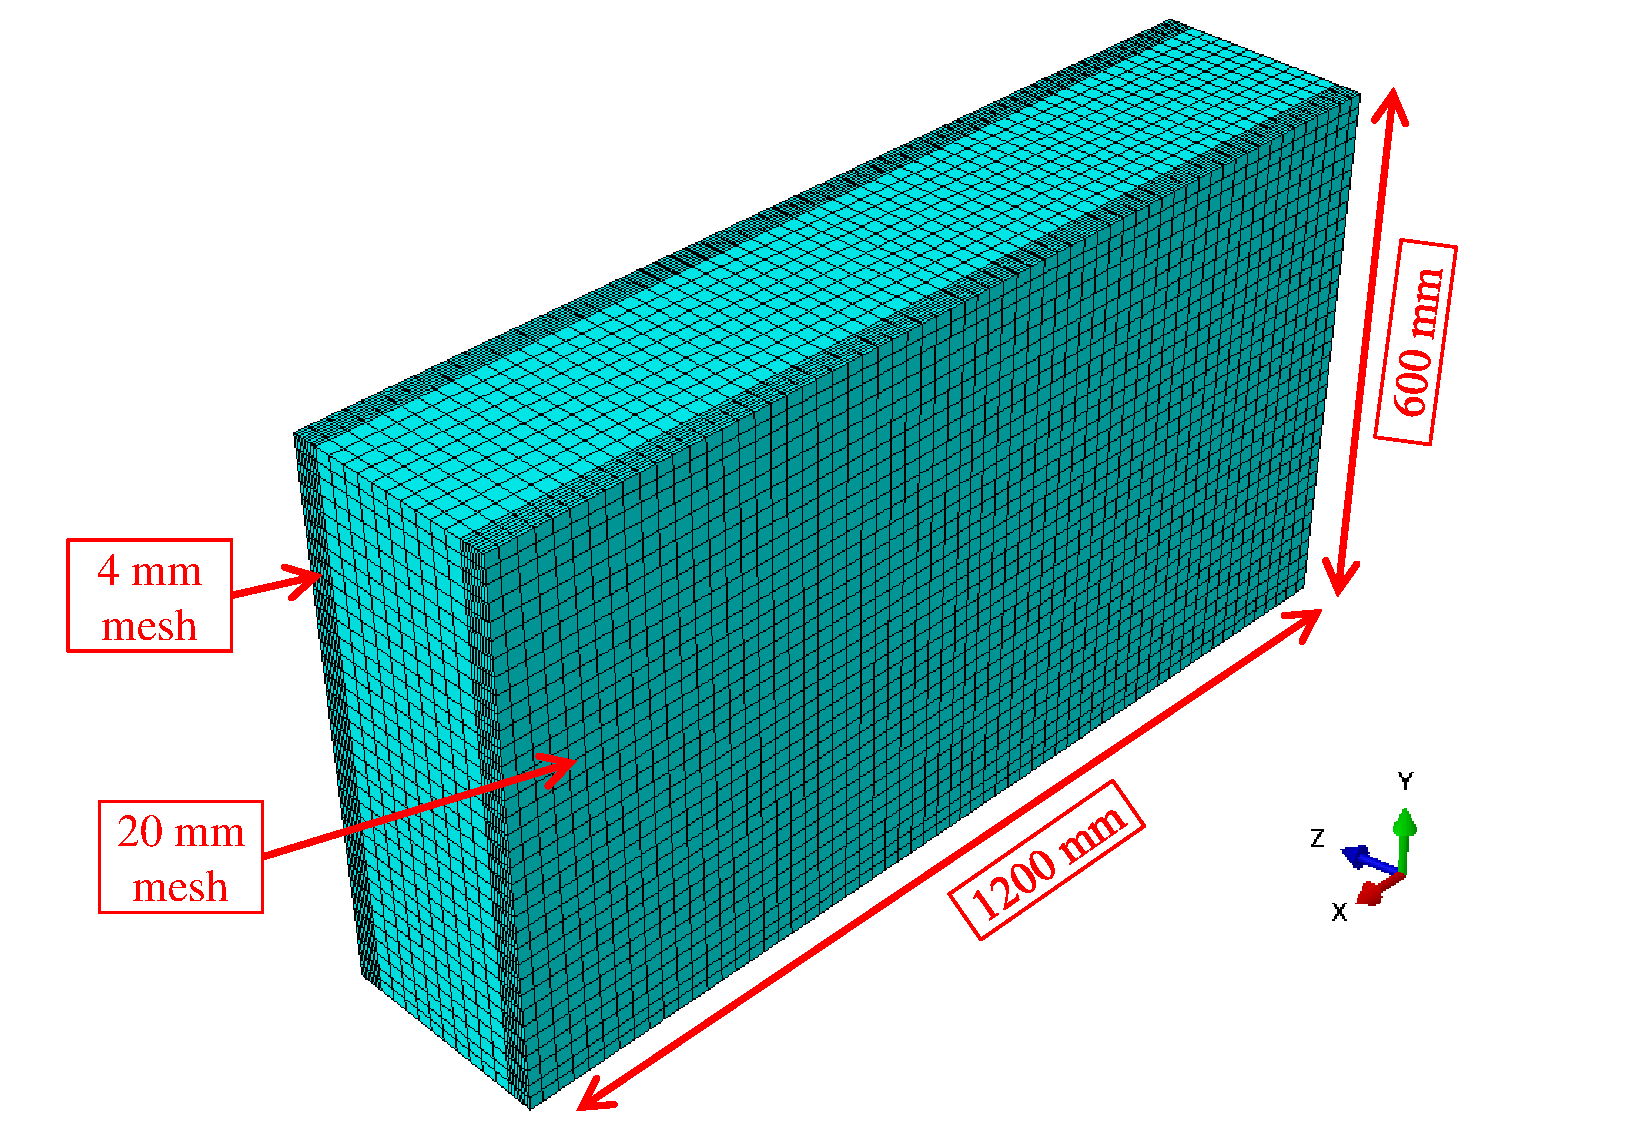
\includegraphics[scale=0.5]{abaqus-typical-mesh.pdf}
		\caption{Mesh arrangement in the thermal model from ABAQUS}
		\label{fig:abaqus-typical-mesh-thermal}
\end{figure}
\begin{figure}[!htbp]
	\centering
		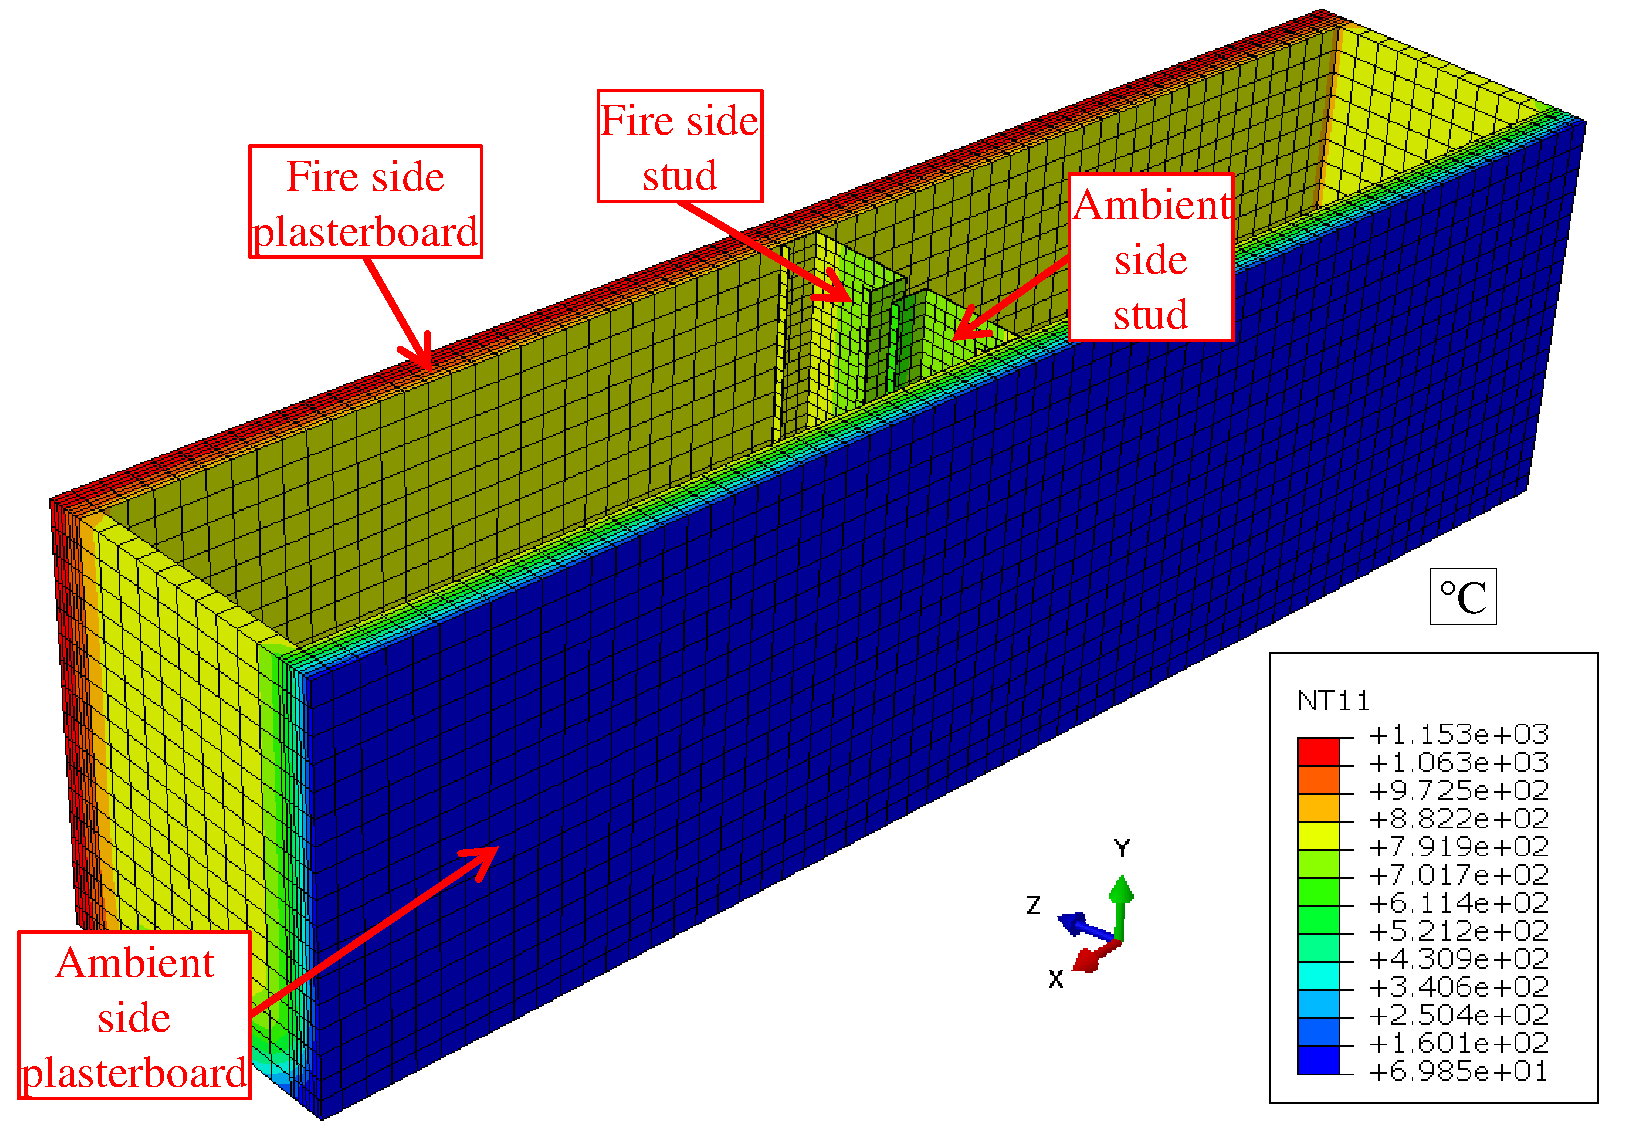
\includegraphics[scale=0.4]{abaqus-typical-output.pdf}
		\caption{Thermal analysis output from ABAQUS}
		\label{fig:abaqus-typical-output}
\end{figure}
\begin{figure}[!htbp]
	\centering
		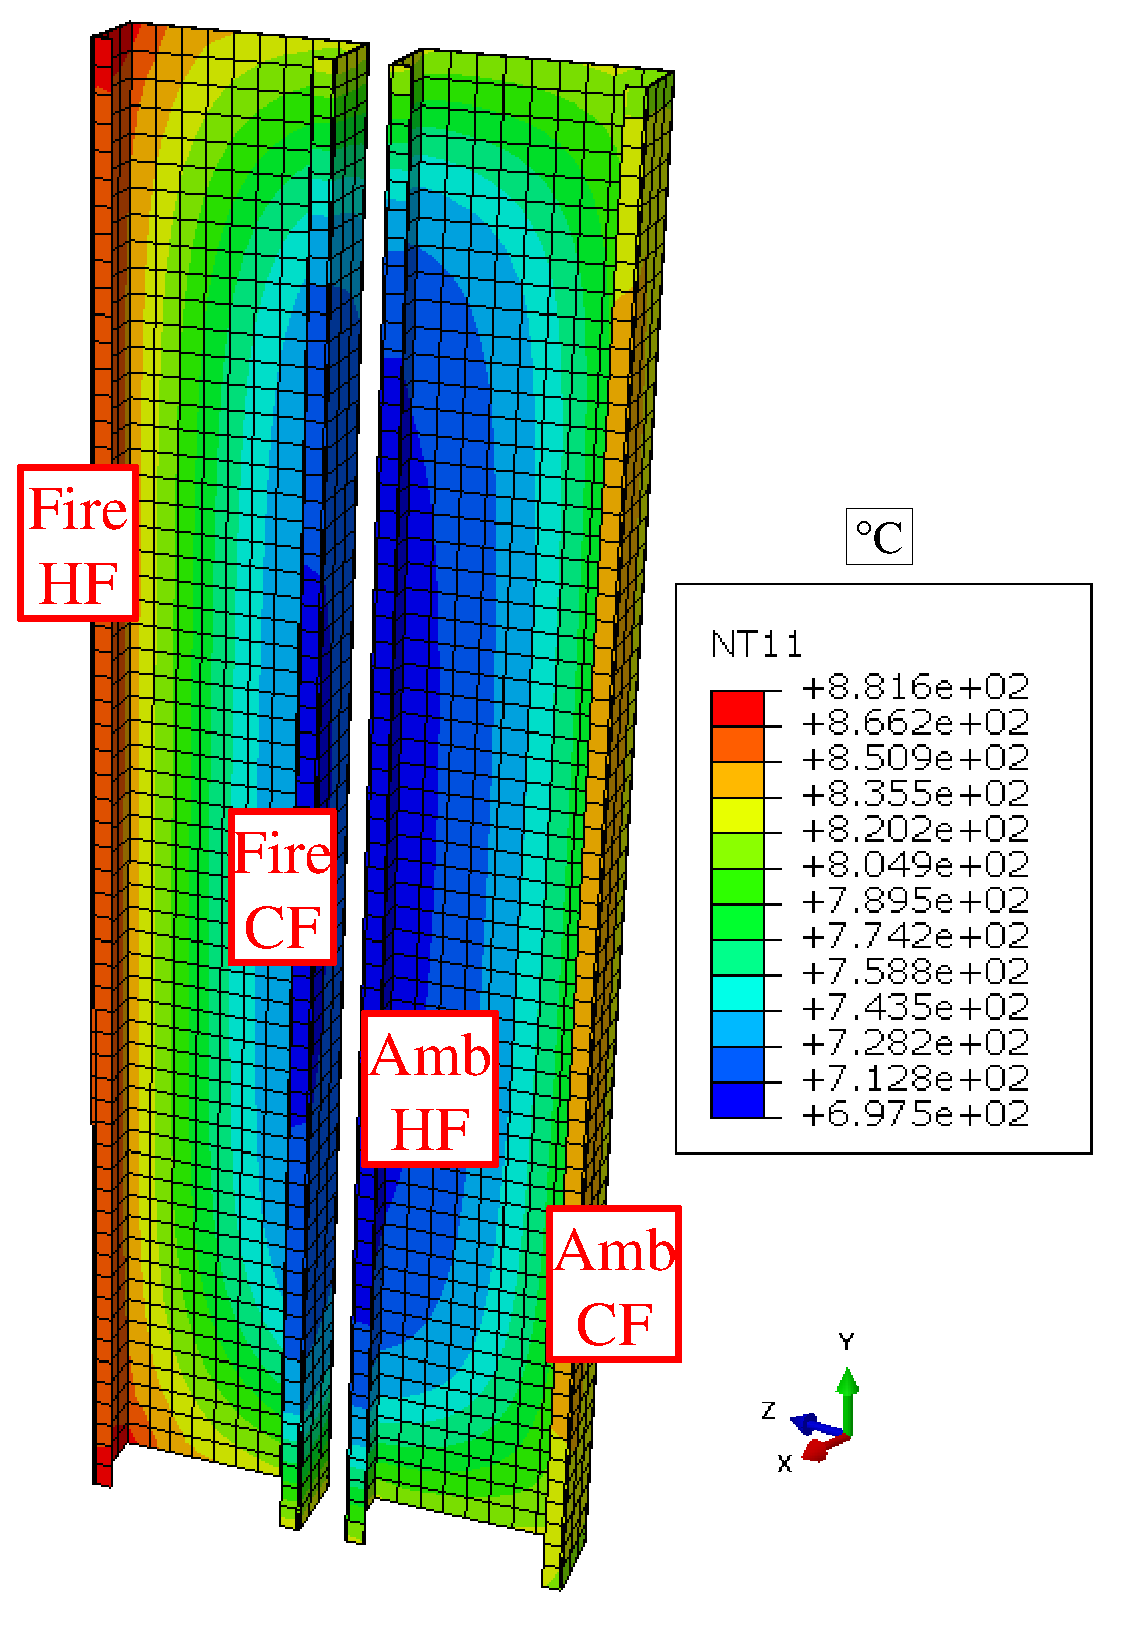
\includegraphics[scale=0.4]{abaqus-typical-output-studs.pdf}
		\caption{Thermal analysis output of studs from ABAQUS}
		\label{fig:abaqus-typical-output-studs}
\end{figure}

\Cref{fig:abaqus-typical-output,fig:abaqus-typical-output-studs} show the thermal analysis output from ABAQUS. It is to be noted that from \Cref{fig:abaqus-typical-output-studs} the temperature distribution is concentrated on the fire side hot flange (Fire-HF) and ambient side cold flange (Amb-CF). This temperature distribution in the studs is unusual in comparison with the time-temperature curves from the experimental studies. The ambient side cold flange is hotter than the ambient side hot flange which means that the heat is transferred to the ambient side plasterboards and then is conducted to the stud flanges as the effects of radiation is considered predominant within the cavity. This assumption does not hold good in the case of non-cavity insulated double stud LSF walls as the order of temperature distribution will be Fire-HF, Fire-CF, Amb-HF and Amb-CF. This hierarchy is clearly evident from the conducted full-scale fire test results in \Cref{ch:Fire}. Further comparisons were made against the time-temperature curves of plasterboards and studs and the discussions are presented next to understand the thermal model predictions.

\Cref{fig:abaqus-output-pb-studs} presents the time-temperature curves of plasterboard from ABAQUS heat transfer analysis. The fire side plasterboard time-temperature curves (Pb1) agree reasonably well with the experimental results. The plateau region present in the time-temperature curve on the fire side plasterboard interface Pb1-Pb2 was not visible in the thermal model predictions. The plateau region in the time-temperature curve present in the experiments is because of the combined effects of radiation and natural convection within the cavity. As the thermal analysis was conducted by assuming only radiation effects within the closed cavity, the thermal model time-temperature curves predicted temperatures higher than the experiments. Both fire and ambient side plasterboard curves (Pb2 and Pb3) from ABAQUS were also higher than the experimental results as this is influenced by the plasterboard interface (Pb1-Pb2) time-temperature curve. The ambient side plasterboard time-temperature curve prediction was also higher in comparison with the experimental results. However, the time-temperature curves of the ambient side plasterboard (Pb4) matched reasonably well with the experimental results as shown in \Cref{fig:abaqus-output-pb-studs} (a).
\begin{figure}[!htbp]
	\centering
	\begin{subfigure}[b]{0.7\textwidth}
		\centering
		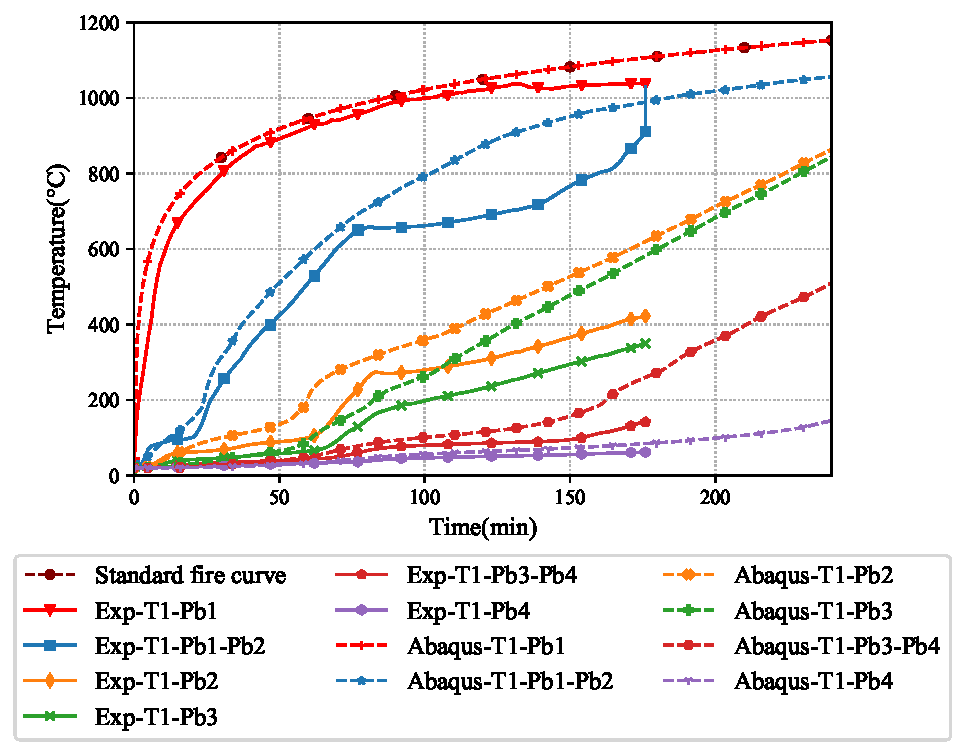
\includegraphics[width=\textwidth]{T1-Plasterboard-Abaqus-vs-Exp-r9.pdf}
		\caption{}
		\label{subfig:T1-Plasterboard-Abaqus-vs-Exp-r9}
	\end{subfigure}
	\begin{subfigure}[b]{0.6\textwidth}
		\centering
		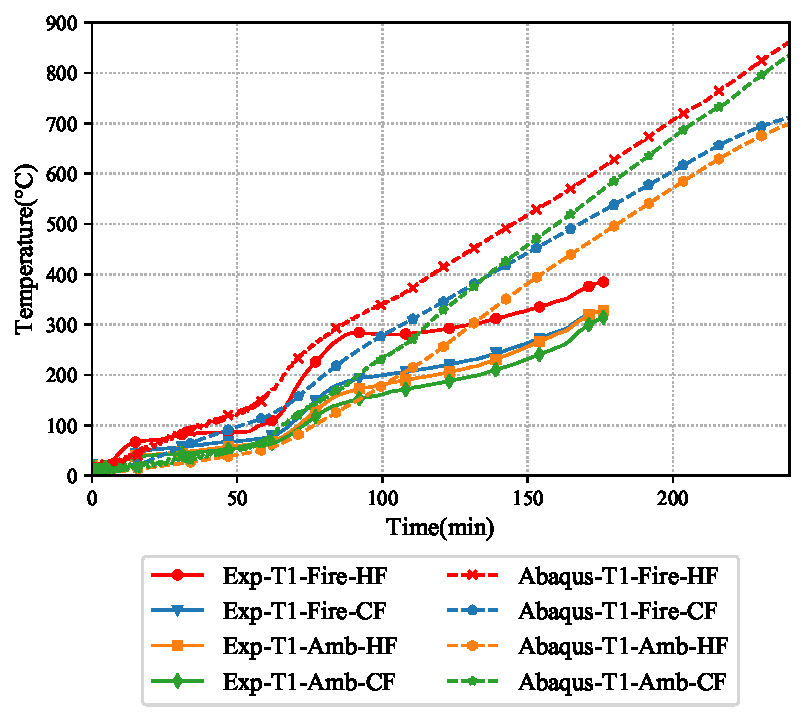
\includegraphics[width=\textwidth]{T1-Stud4-Mid-Abaqus-vs-Exp-r9.pdf}
		\caption{}
		\label{subfig:T1-Stud4-Mid-Abaqus-vs-Exp-r9}
	\end{subfigure}
	   \caption{Comparison of time-temperature curves from ABAQUS thermal analysis and experiments (a) Average plasterboard temperatures (b) Stud4-Mid temperatures}
	   \label{fig:abaqus-output-pb-studs}
\end{figure}

The stud time-temperature curves are presented in \Cref{subfig:T1-Stud4-Mid-Abaqus-vs-Exp-r9}. The hot and cold flanges matched reasonably well till 60 min of the fire test. However, the time-temperature curves exhibited steep rise after 60 min. This indicates that the cooling effect experienced in the stud hot and cold flanges from experiments could not be simulated by the developed ABAQUS thermal model. The ambient side cold flange (T1-Abaqus-Amb-CF) time-temperature curve was higher than the ambient side hot flange (T1-Abaqus-Amb-HF) as shown in \Cref{subfig:T1-Stud4-Mid-Abaqus-vs-Exp-r9}, which is unusual. However, this discrepancy was not present in SAFIR thermal analysis. This is also partly because the stud rows in Test-T1 are located 20 mm apart, resulting in no heat transfer through conduction during the fire test. As the heat transfer within the cavity is assumed to be dominated by radiation in the ABAQUS heat transfer model, the time-temperature curves on the ambient side hot and cold flanges mismatch in comparison with the experimental results. Similar to SAFIR heat transfer analysis results, the time-temperature curves of studs from ABAQUS thermal analysis were significantly higher than the experimental results. The complex heat transfer effects of convection combined with radiation within the cavity were not accounted for in the single stud wall thermal models developed using SAFIR and ABAQUS. Therefore, it becomes a necessity to develop a thermal model which can account for the combined convection and radiation effects within the cavity and simulate more accurately the thermal behaviour of the complex LSF walls systems.

\section{Thermal modelling in FDS}

Unlike other FE packages in which the thermal models of LSF walls are readily available, very limited literature is available on the thermal models of LSF walls developed in FDS except in research studies conducted by \citet{Lazaro2016,Lazaro2018,Nguyen2018}. Thermal FE models in FDS had to be generated for this research study to predict the time-temperature profile of the complex LSF walls. The previous FDS model considered in the literature assumed the LSF wall as a homogenous entity and the thermal models were created with single obstruction (\&OBST) comprising of studs and plasterboards. However, this approach cannot be employed in the present study as the individual time-temperature curves from the studs are necessary to predict the structural behaviour of the LSF wall under fire. Therefore, the plasterboards and studs were modelled separately to depict the experimental set-up. 

Past literature considered different model dimensions based on their experimental set-up. The model dimensions varied form 50 $\times$ 50 mm to 3 $\times$ 3 m. Likewise, the mesh density also varied from 5 to 50 mm (\citet{Lazaro2018,Nguyen2018}). This assumption was best suitable as the time-temperature curves were measured on the fire exposed and ambient sides only in the above-mentioned research studies. However, these studies did not model the structural behaviour of the wall. To develop the current thermal model based on past literature, a sensitivity analysis was conducted initially to determine the effects of the model dimensions. Also, in the sensitivity analyses the obstructions (\&OBST) were modelled as solid entity, which was found to add complexity to the model resulting in higher computational time. Therefore, a simplistic approach of modelling the obstructions as 2D entity was chosen in this research study to model the complex LSF walls. 

\subsection{Thermal model description in FDS}

The models were created in the command line interface using Notepad ++ a general purpose text editor. However, PyroSim was used for pre-processing the models in certain instances to consolidate meshes in the boundary. SmokeView was used for post processing and visualising the thermal model results. Output from the thermal models were saved on to a CSV file, which was later used for plotting the time-temperature curves. Certain assumptions were used in creating the FDS thermal model. The models were created with the appropriate depth of the test wall used in the experiments. However, the height and width of the model was restricted to 200 mm. The variation in heat transfer along the height of the test wall was ignored for simplifying the model. This is because, the standard time-temperature curve is specified as the input boundary condition to the entire fire exposed surface (Pb1) using the vent function (\&VENT) in FDS. This implies that, the temperature input is uniform throughout the surface and the variation in temperature which occurs in the experiments due to difference in furnace burner temperatures can be assumed insignificant and ignored in the current model, as the comparison is made against the average time-temperature curve achieved in the furnace. It is to be noted that the ISO 834 time-temperature curve is specified as the input boundary condition on the fire side plasterboard in ABAQUS and SAFIR thermal models. However, in FDS it is specified through a \&VENT surface, which provides the leverage to simulate the standard fire curve from furnace similar to the full-scale fire tests. This might result in a small difference between the incident fire side plasterboard (Pb1) temperature and the standard fire curve due to the small distance between the \&VENT surface and the Pb1 surface. This small difference in temperatures will still be within the permissible limits of 100\degree C as per AS 1530.4 (\citet{StandardsAustral2014}) and can be ignored.
\begin{figure}[!htbp]
	\centering
		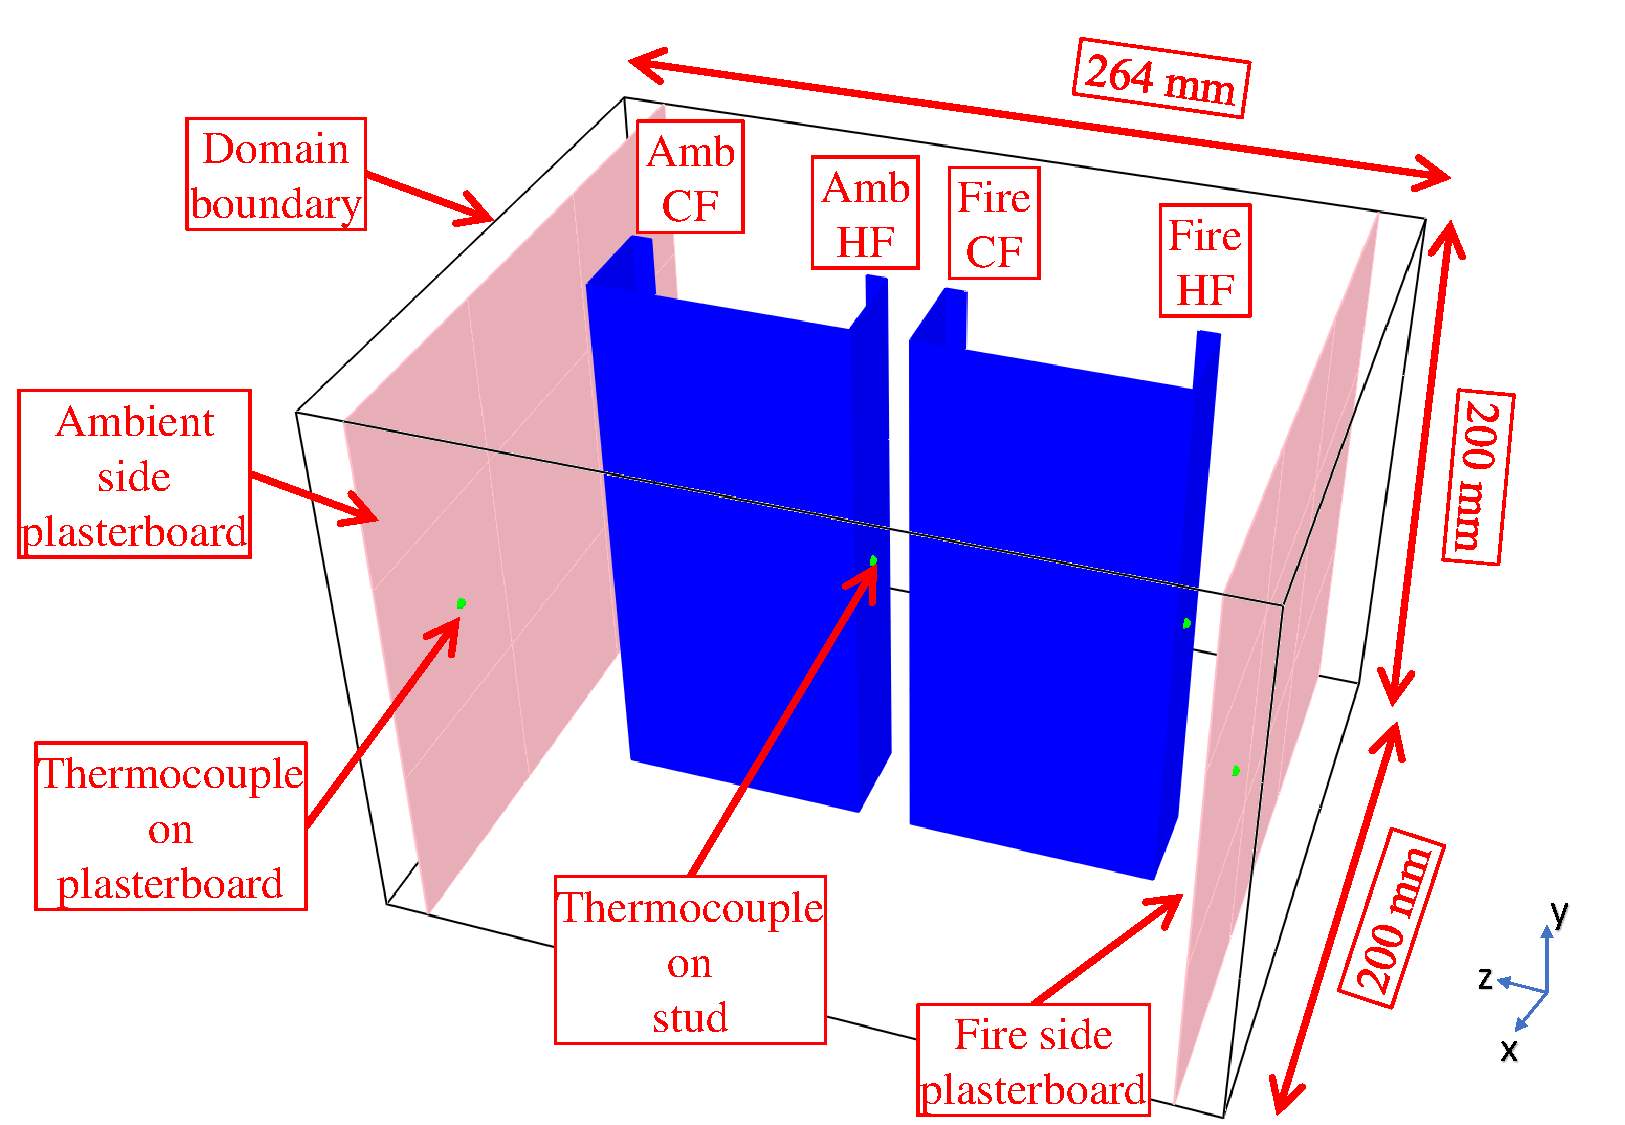
\includegraphics[width=10cm, height=8cm]{fds-typical-model.pdf}
		\caption{Model of Double Stud LSF Wall Panel}
		\label{fig:fds-typical-model}
\end{figure}

Considering the above mentioned findings, the obstructions in the model followed ``1 cell thick" rule of FDS as shown in \Cref{fig:fds-typical-model}. The temperature dependent material properties for gypsum plasterboards, steel studs and glass fibre insulation for the thermal analysis were taken from \citet{Rusthi2017}. The temperature dependent material properties were used for conductivity and specific heat only. Temperature-dependant material properties were specified to the model using \&RAMP function in the FDS input file. The density was kept constant at 768.5kg/m\(^3\) for plasterboard, 7850 kg/m\(^3\) for steel and 11 kg/m\(^3\) for glass fibre insulation. An emissivity of 0.9 was used for the plasterboards while the emissivity used for the steel stud was 0.7. The model was enclosed in a domain boundary with 16 mm mesh based on the sensitivity analyses, matching the plasterboard thickness. Convective heat transfer co-efficient of 25 W/m$^2$\degree C was considered for the fire side plasterboard surface while it was 10 W/m$^2$\degree C for the ambient side plasterboard surface. AS 1530.4 (\citet{StandardsAustral2014}) standard fire curve (identical to \citet{iso834} curve) was specified as the input boundary condition to replicate the fire side using \&VENT function. The domain boundary was created in close contact with the model to prevent any heat loss around the model sides during simulation. The domain boundary was closed in all directions and adiabatic boundary conditions were specified representing no heat transfer through the sides. The boundary facing the ambient side was alone kept open to simulate the natural convection from the ambient side plasterboard surface. As ``1-cell thick" modelling technique was used, no contact was established between the studs and plasterboards. However, corresponding thickness was specified on the surface line using the \&SURF function. Temperatures were measured across the model using the \&DEVC function at various locations similar to thermocouples and the corresponding time-temperature curves are plotted. The thermal model analysis was carried out for a time period of 240 min for all the conducted full-scale fire test configurations. The time-temperature curves from the FDS model and experiment are compared and discussed in the next section.  

\subsection{Thermal model validation - Non-cavity insulated Tests-T1, T2, T3, T4, T8 and T9}

The thermal model was created with a height and width of 200 mm while the depth of the model was 264 mm similar to the full-scale fire Test-T1 of a double stud wall mage of 90 $\times$ 0.95 mm studs with a load ratio of 0.4. The thermal analysis was carried out for a time period of 240 min. \Cref{fig:T1-fds-model} shows the thermal model of Test-T1 with 16 mm meshes. The boundary domain was  subdivided to nine regions to facilitate parallel processing in the HPC cluster. Through this the thermal model could be solved in 26 min, which is a considerable optimisation in the computational time in comparison with SAFIR and ABAQUS thermal models.   
\begin{figure}[!htbp]
	\centering
		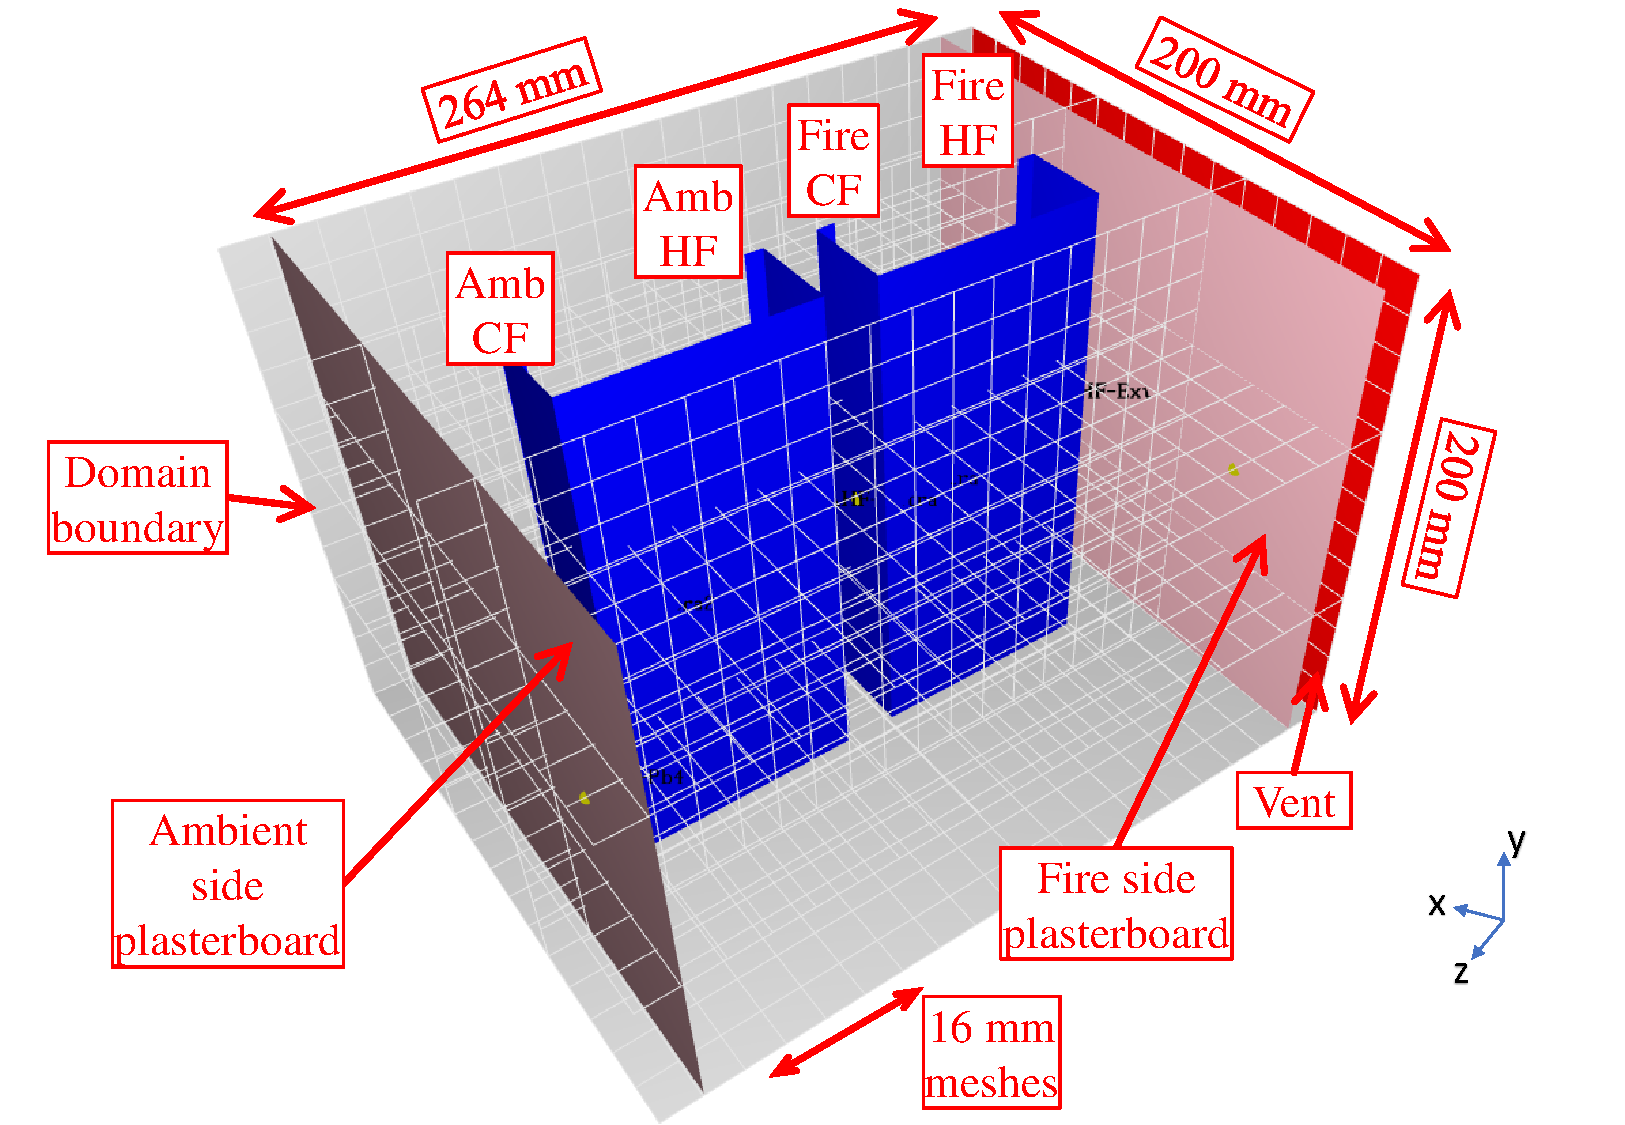
\includegraphics[scale=0.35]{T1-fds-model.pdf}
		\caption{Thermal model of Test-T1 wall}
		\label{fig:T1-fds-model}
\end{figure}
\begin{figure}[!htbp]
	\centering
	\begin{subfigure}[b]{0.45\textwidth}
		\centering
		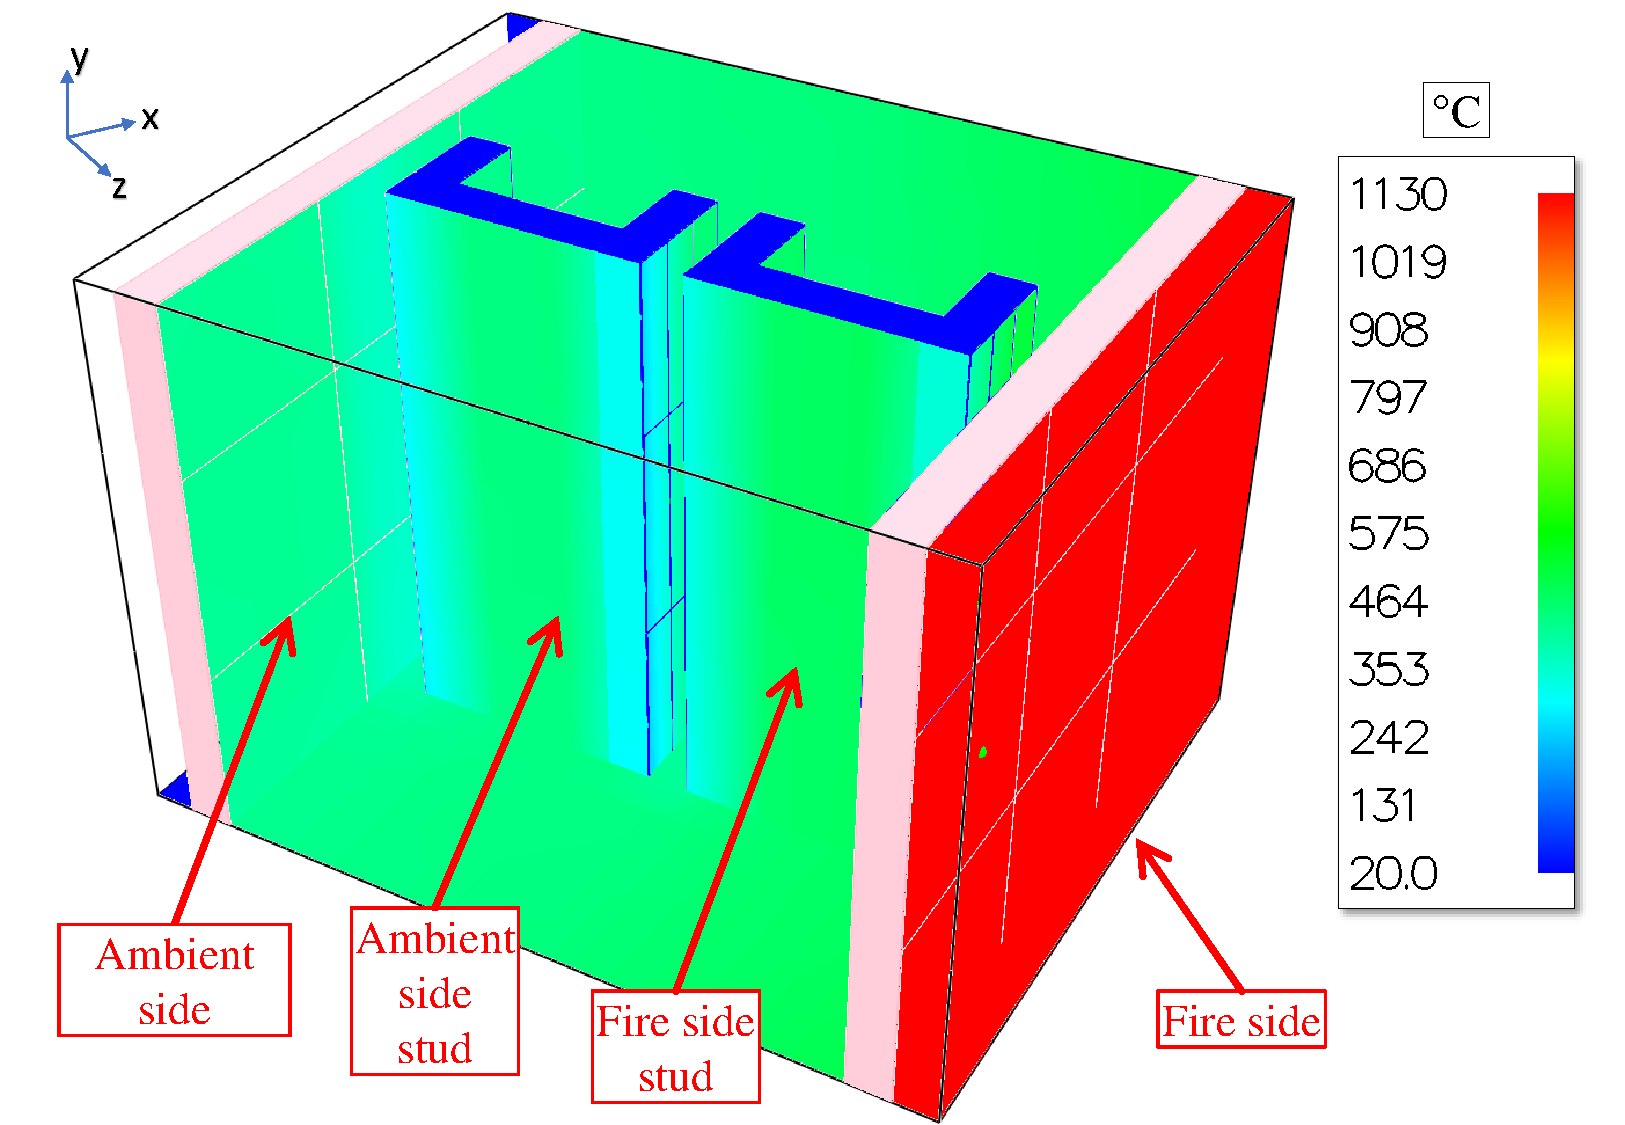
\includegraphics[width=\textwidth]{T1-fds-output.pdf}
		\caption{}
		\label{subfig:T1-fds-output}
	\end{subfigure}
	\begin{subfigure}[b]{0.45\textwidth}
		\centering
		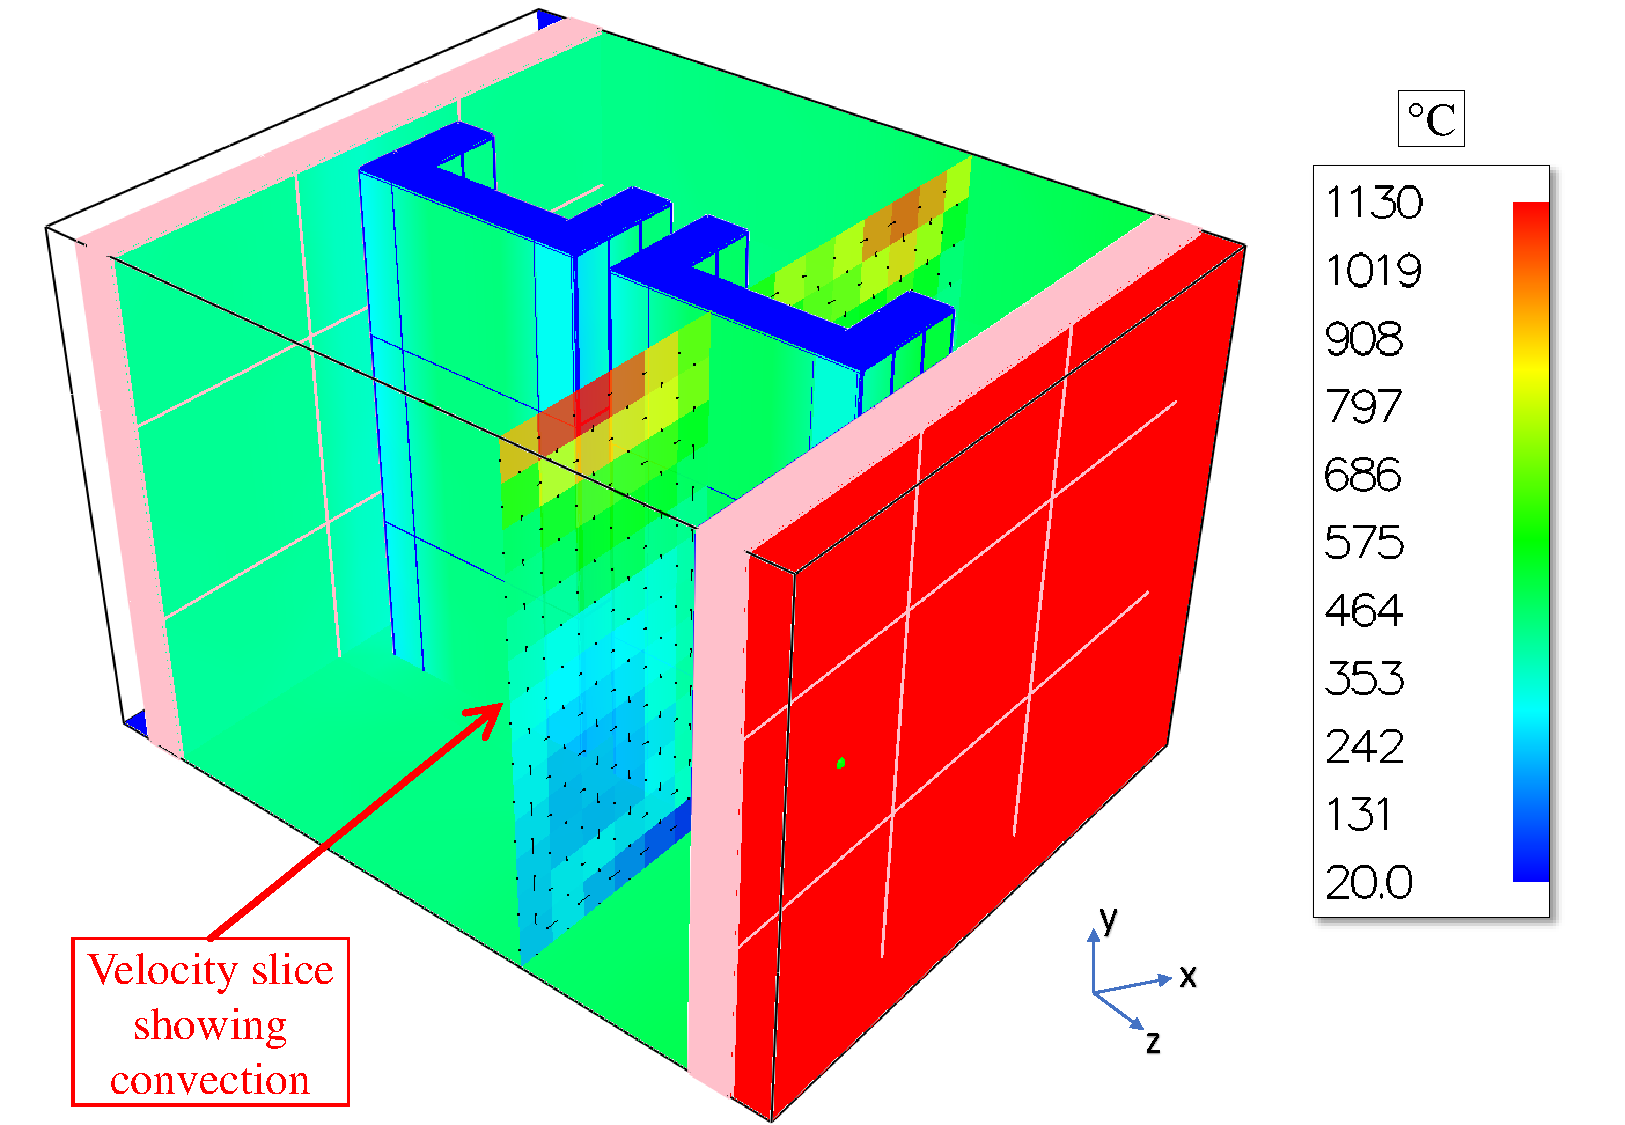
\includegraphics[width=\textwidth]{T1-fds-output-velocity-slice.pdf}
		\caption{}
		\label{subfig:T1-fds-output-velocity-slice}
	\end{subfigure}
	   \caption{Output from FDS thermal analysis (a) Temperature profile (b) Velocity slice for convection}
	   \label{fig:abaqus-output-pb-studs}
\end{figure}

Temperature profile and velocity slice from FDS thermal model are shown in Figures \ref{fig:abaqus-output-pb-studs} (a) and (b). Time-temperature curves of plasterboard from FDS thermal analysis are compared against experimental results and are presented in \Cref{subfig:T1-r61-Pb-Fds-vs-Exp}.  Fire side time-temperature curve (Fds-T1-Pb1) exhibited good agreement with the ISO 834 time-temperature curve. Plasterboard interface time-temperature curve (Fds-T1-Pb1-Pb2) exhibited a reasonable agreement with the experimental results till 75 min of fire test. The plateau region experienced in the fire test time-temperature curve was not significantly noticeable in the FDS thermal analysis prediction. The occurrence of plateau region between the plasterboard interface is attributed to the factors such as wider cavity depth, natural convection together with radiation effects, discontinuous stud arrangement, and moisture movement within the plasterboard. Except for the effects of moisture movement, all the other effects were accounted for in the current thermal model. However, the combined effects along with the moisture movement between the plasterboard interface could not be simulated due to the complexity in the modelling technique and is beyond the scope of this research study. But, the model was able to successfully incorporate the effects of convection within the cavity due to the change in the air temperature within the cavity. This is evident from the time-temperature curve of fire side plasterboard interface surfaces as shown in \Cref{subfig:T1-r61-Pb-Fds-vs-Exp}. Unlike a steep increase in the Pb1-Pb2 time-temperature from SAFIR and ABAQUS a change in slope is noticeable from the FDS thermal analysis prediction as shown in \Cref{fig:fe-model-output-comparison}. This confirms that the developed FDS model could better predict the thermal behaviour of non-cavity insulated double stud LSF walls. The time-temperature curve of the fire side cavity surface from the thermal model (Fds-T1-Pb2) was higher than the experimental curve. However, the ambient side cavity (Pb3), the ambient side plasterboard interface (Pb3-Pb4) and the ambient side plasterboard surface time-temperature curve predictions exhibited reasonable agreement with the experimental results.
\begin{figure}[!htbp]
	\centering
	\begin{subfigure}[b]{0.7\textwidth}
		\centering
		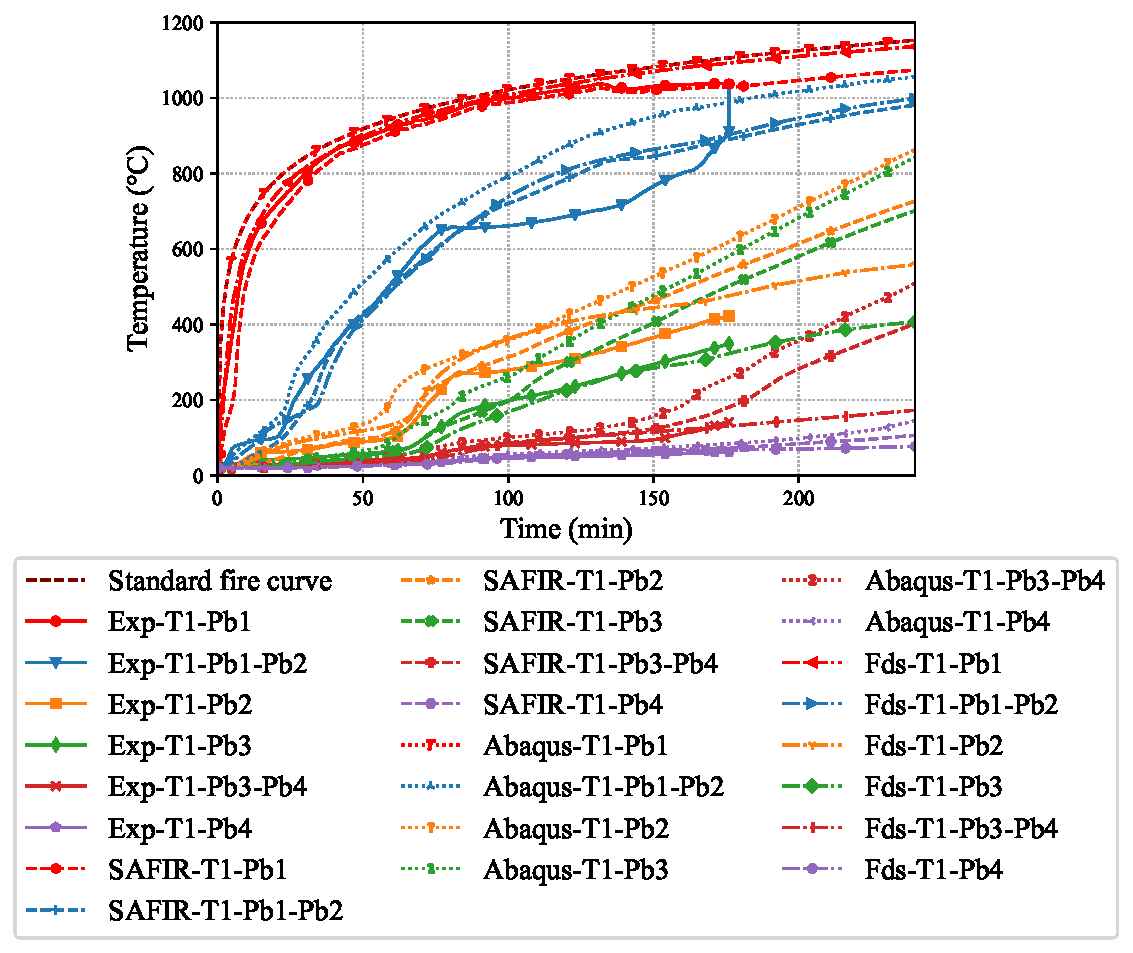
\includegraphics[width=\textwidth]{T1-Plasterboard-fe-comparison.pdf}
		\caption{}
		\label{subfig:T1-Plasterboard-fe-comparison}
	\end{subfigure}
	\begin{subfigure}[b]{0.6\textwidth}
		\centering
		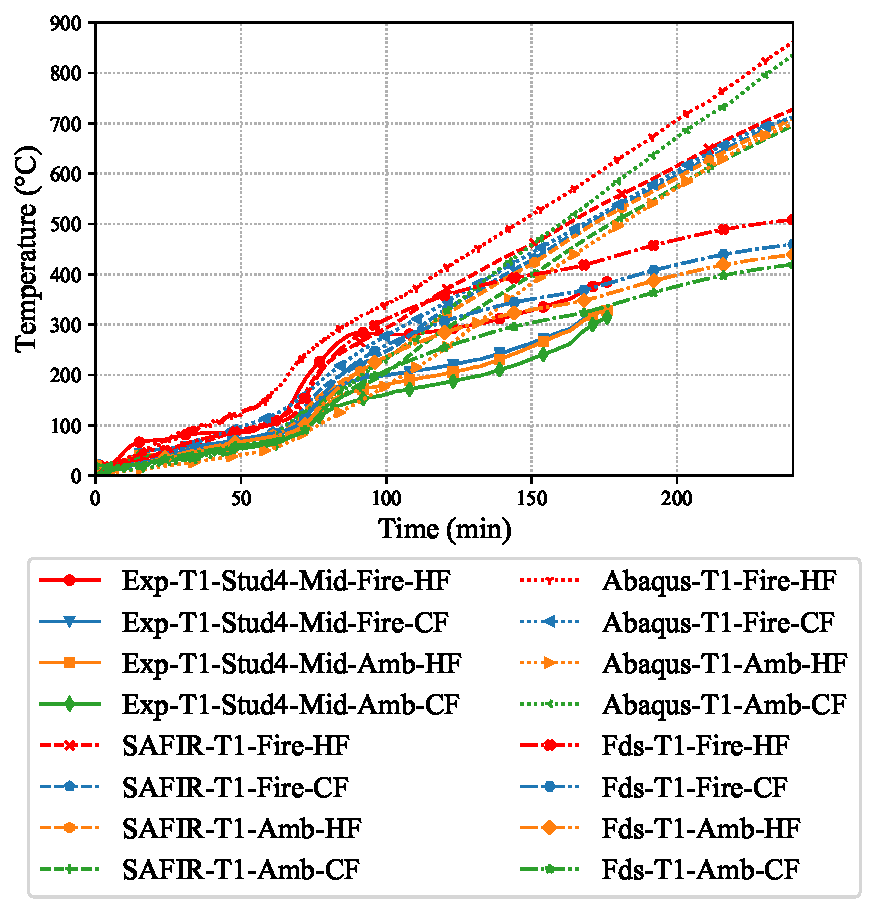
\includegraphics[width=\textwidth]{T1-Studs-4-fe-comparison.pdf}
		\caption{}
		\label{subfig:T1-Studs-4-fe-comparison}
	\end{subfigure}
	   \caption{Comparison of time-temperature curves from experiment, SAFIR, FDS and ABAQUS models for Test-T1 (a) Average Plasterboard (b) Stud4-Mid}
	   \label{fig:fe-model-output-comparison}
\end{figure}
\begin{figure}[!htbp]
	\centering
	\begin{subfigure}[b]{0.7\textwidth}
		\centering
		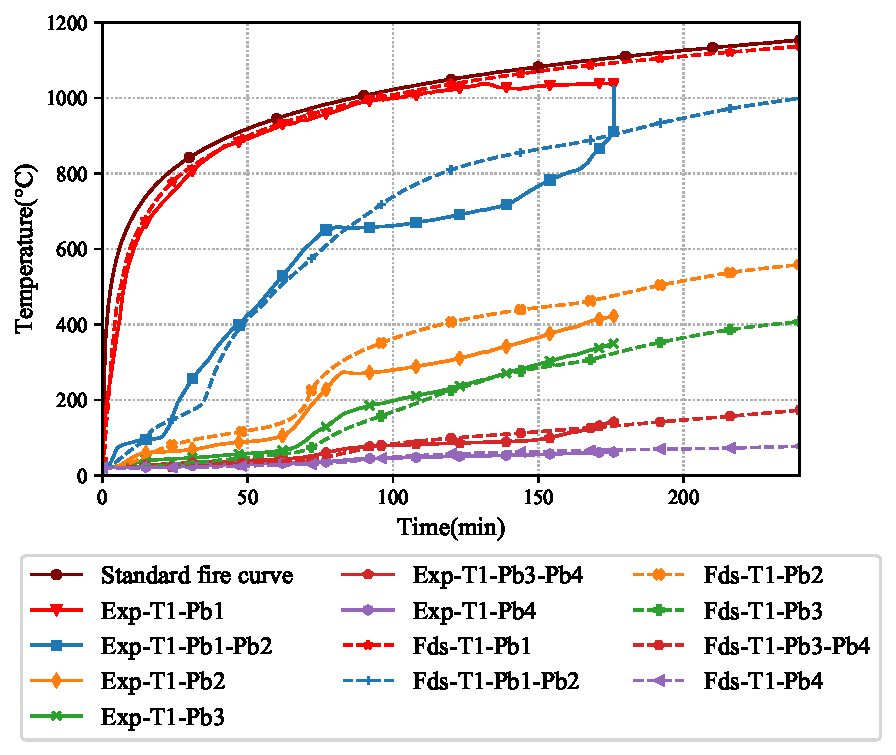
\includegraphics[width=\textwidth]{T1-r61-Pb-Fds-vs-Exp.pdf}
		\caption{}
		\label{subfig:T1-r61-Pb-Fds-vs-Exp}
	\end{subfigure}
	\begin{subfigure}[b]{0.6\textwidth}
		\centering
		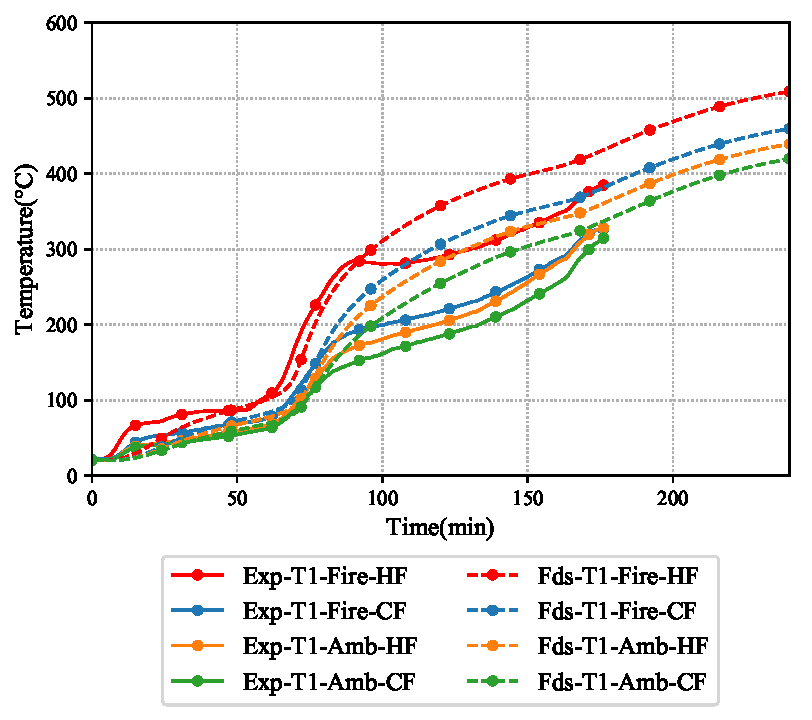
\includegraphics[width=\textwidth]{T1-r61-Studs-4-Fds-vs-Exp.pdf}
		\caption{}
		\label{subfig:T1-r61-Studs-4-Fds-vs-Exp}
	\end{subfigure}
	   \caption{Comparison of time-temperature curves from experiment and FDS model for Test-T1 (a) Average Plasterboard (b) Stud4-Mid}
	   \label{fig:fds-output-pb-studs-t1}
\end{figure}

Stud time-temperature curves shown in \Cref{subfig:T1-r61-Studs-4-Fds-vs-Exp} also exhibited good agreement with the experimental results till 75 min of the fire test. The increase in slope experienced in the time-temperature curves from 50 min of the experimental results could also be simulated by the developed thermal model with reasonable accuracy. However, as the fire side cavity (Pb2) plasterboard time-temperature curve predicted temperatures higher than the experiments, similar effects were noticeable in the stud hot and cold flanges wherein the predicted hot and cold flange time-temperature curves were marginally higher than the experimental results. The maximum temperature recorded by the fire side hot flange on Stud3-Mid (Exp-T1-Fire-HF) at the end of the fire test at 176 min was 395\degree C while the predictions from FDS thermal model was 431\degree C. i.e., a difference of 8.35\% (36\degree C). This can be considered as negligible in relation to the use of stud hot flange temperatures in  structural failure time predictions. 
\begin{figure}[!htbp]
	\centering
	\begin{subfigure}[b]{0.7\textwidth}
		\centering
		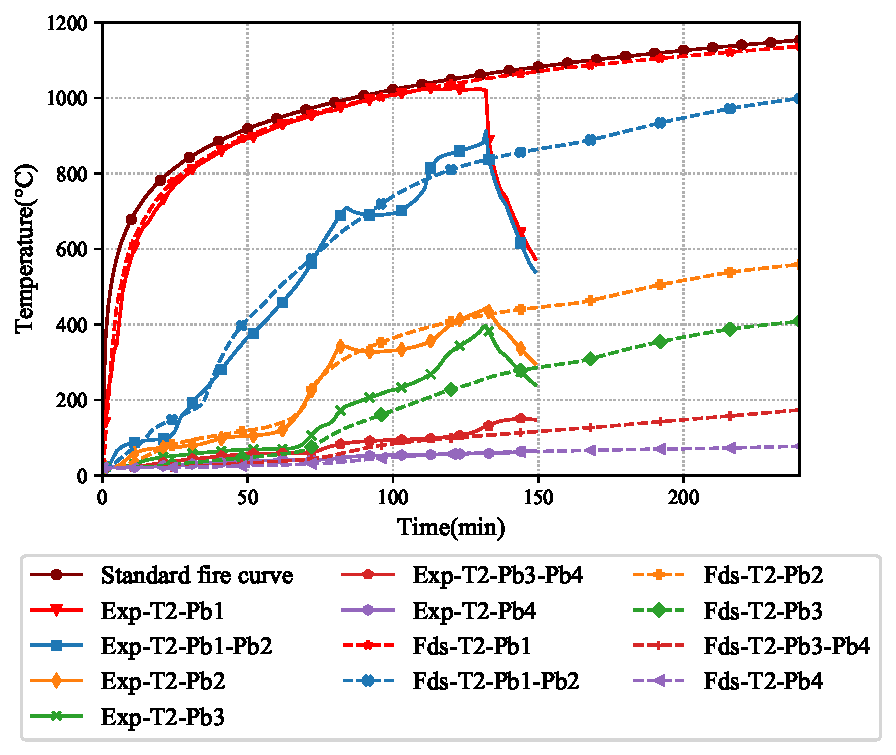
\includegraphics[width=\textwidth]{T2-r0-Pb-Fds-vs-Exp.pdf}
		\caption{}
		\label{subfig:T2-r0-Pb-Fds-vs-Exp}
	\end{subfigure}
	\begin{subfigure}[b]{0.6\textwidth}
		\centering
		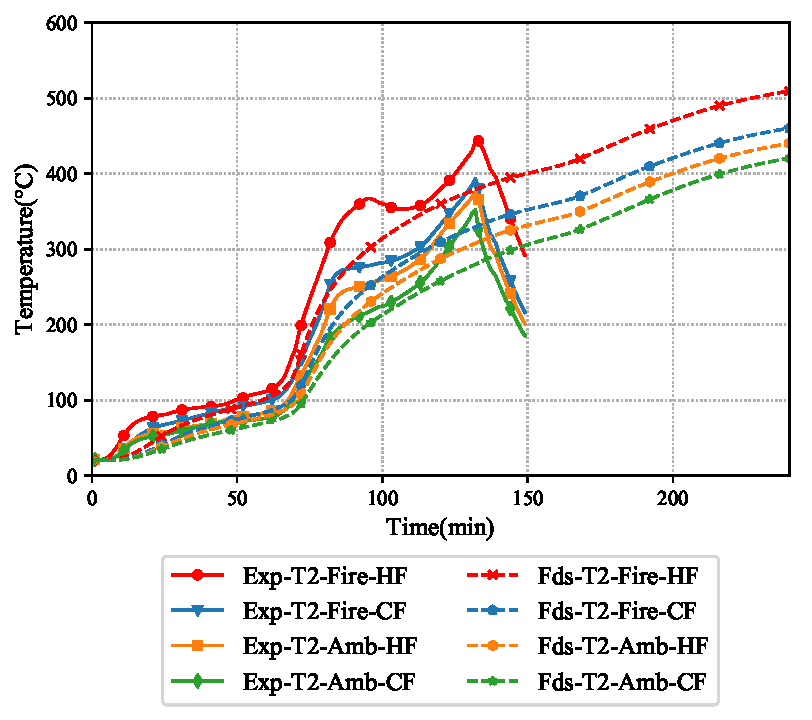
\includegraphics[width=\textwidth]{T2-r0-Studs-3-Fds-vs-Exp.pdf}
		\caption{}
		\label{subfig:T2-r0-Studs-3-Fds-vs-Exp}
	\end{subfigure}
	   \caption{Comparison of time-temperature curves from experiment and FDS model for Test-T2 (a) Average Plasterboard (b) Stud3-Mid}
	   \label{fig:fds-output-pb-studs-t2}
\end{figure}

\Cref{subfig:T2-r0-Pb-Fds-vs-Exp} compares the plasterboard time-temperature curves for Test-T2 of a double stud wall made of 90 $\times$ 0.75 mm studs. The plasterboard time-temperature curves exhibited reasonable agreement except for T2-Pb3 where the FDS model predictions were less than the experimental results. However, the ambient side plasterboard surface time-temperature curves also agreed reasonably well. Stud time-temperature curves agreed well till 60 min of the fire test as shown in \Cref{subfig:T2-r0-Studs-3-Fds-vs-Exp}. The steep increase experienced in the Exp-T2-Fire-HF could not be simulated in the FDS model as this was a resultant of localised plasterboard open up in the fire test. The temperature recorded at 132 min in Exp-T2-Fire-HF was 444\degree C while it was 380\degree C from the FDS model, i.e., FDS model prediction of the stud hot flange temperature was 64 \degree C less than the experimental results. Similarly difference in the fire side cold temperature was 62\degree C (393-331\degree C). The fire side hot and cold flange temperatures are 14.4\% and 15.77\% less than the corresponding experimental results of Test-T2. This may be partly due to the plasterboard fall-off on the fire side plasterboard during the fire test as reported in \Cref{sec:t2-results} of \Cref{ch:Fire}.
\begin{figure}[!htbp]
	\centering
	\begin{subfigure}[b]{0.7\textwidth}
		\centering
		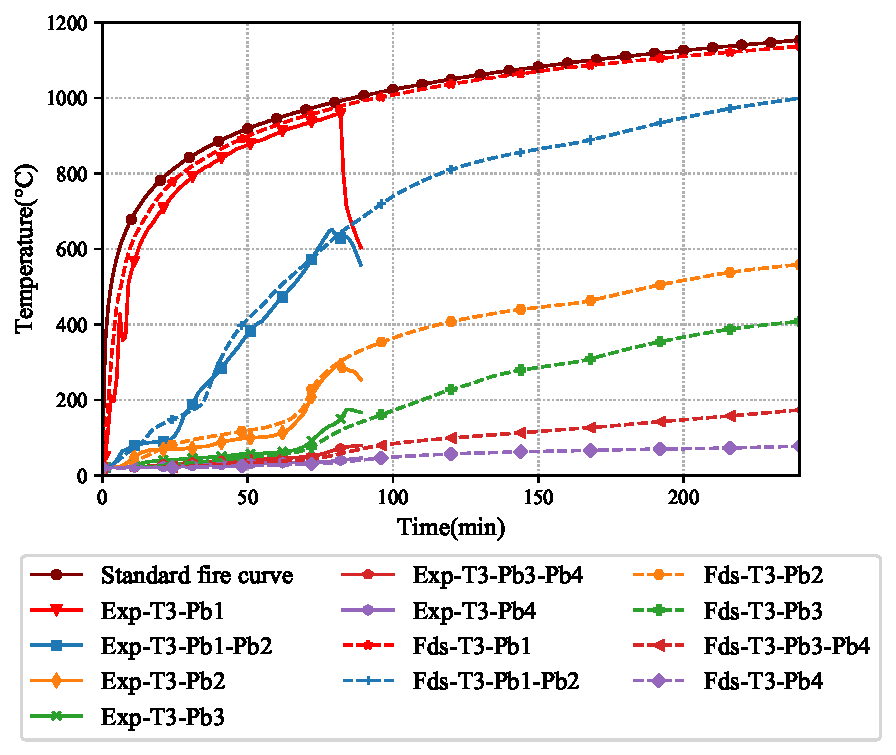
\includegraphics[width=\textwidth]{T3-r0-Pb-Fds-vs-Exp.pdf}
		\caption{}
		\label{subfig:T3-r0-Pb-Fds-vs-Exp}
	\end{subfigure}
	\begin{subfigure}[b]{0.6\textwidth}
		\centering
		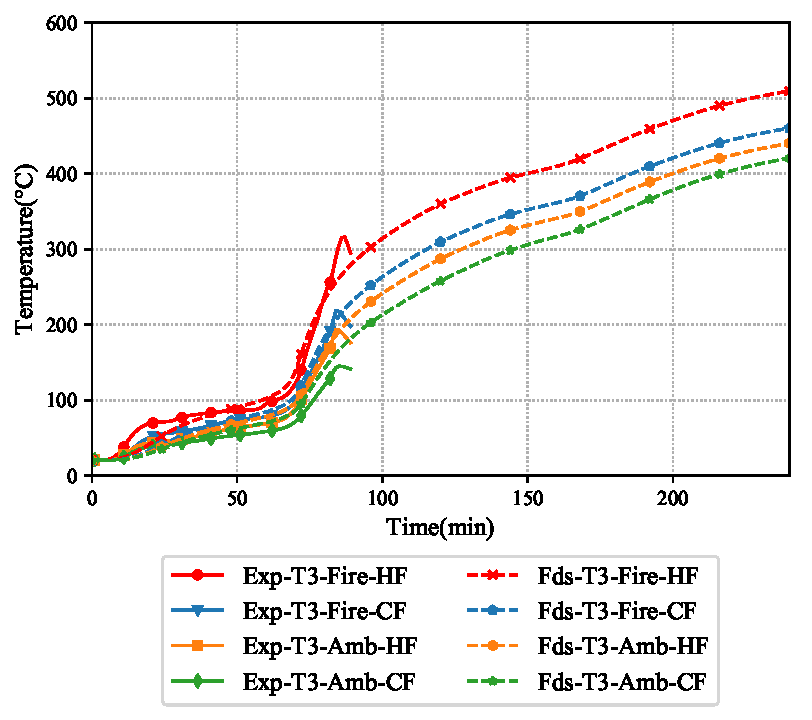
\includegraphics[width=\textwidth]{T3-r0-Studs-4-Fds-vs-Exp.pdf}
		\caption{}
		\label{subfig:T3-r0-Studs-4-Fds-vs-Exp}
	\end{subfigure}
	   \caption{Comparison of time-temperature curves from experiment and FDS model for Test-T3 (a) Average Plasterboard (b) Stud4-Mid}
	   \label{fig:fds-output-pb-studs-t3}
\end{figure}

As Test-T3 was conducted on a double stud wall made of 90 $\times$ 0.75 mm studs but with a higher load ratio (0.6) the time-temperature curves from the experiment are limited to 81 min. However, the FDS thermal analysis predictions were carried out for 240 min. \Cref{subfig:T3-r0-Pb-Fds-vs-Exp} (a) shows the plasterboard time-temperature curve validation against experimental results. All the plasterboard time-temperature curves exhibit good agreement with the experimental results. This is further evident from the stud time-temperature curves shown in \Cref{subfig:T3-r0-Studs-4-Fds-vs-Exp}.
\begin{figure}[!htbp]
	\centering
	\begin{subfigure}[b]{0.7\textwidth}
		\centering
		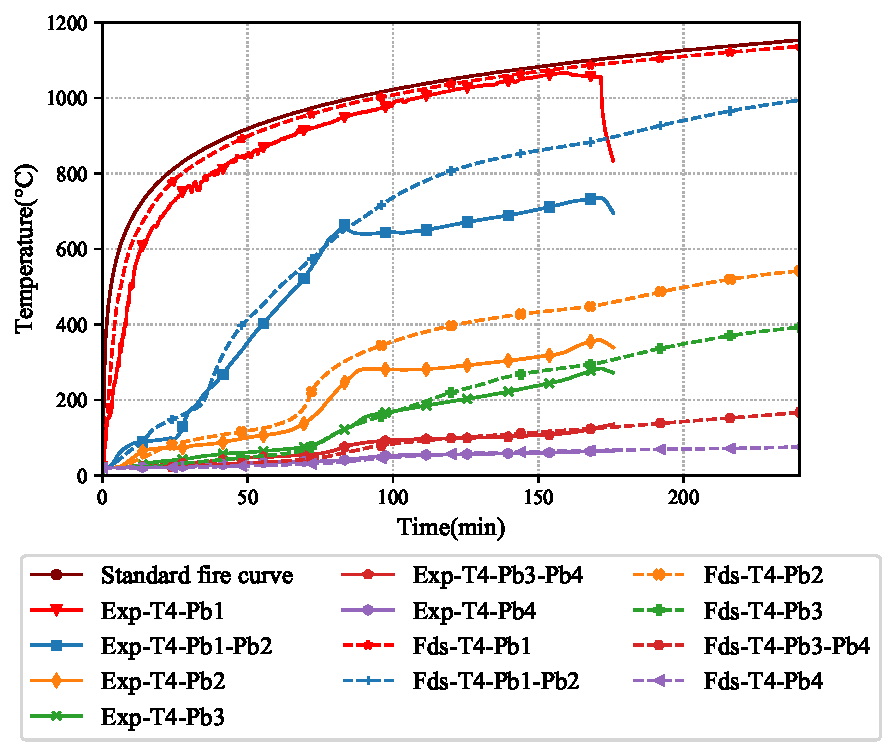
\includegraphics[width=\textwidth]{T4-r0-Pb-Fds-vs-Exp.pdf}
		\caption{}
		\label{subfig:T4-r0-Pb-Fds-vs-Exp}
	\end{subfigure}
	\begin{subfigure}[b]{0.6\textwidth}
		\centering
		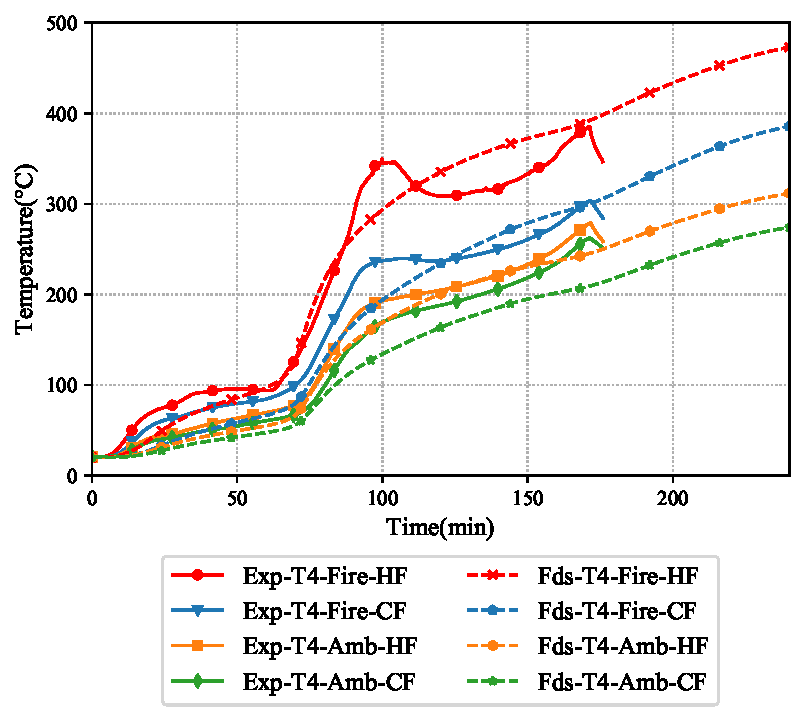
\includegraphics[width=\textwidth]{T4-r0-Studs-3-Fds-vs-Exp.pdf}
		\caption{}
		\label{subfig:T4-r0-Studs-3-Fds-vs-Exp}
	\end{subfigure}
	   \caption{Comparison of time-temperature curves from experiment and FDS model for Test-T4 (a) Average Plasterboard (b) Stud3-Mid}
	   \label{fig:fds-output-pb-studs-t4}
\end{figure}

Test-T4 was conducted on a double stud wall with 70 $\times$ 0.95 mm studs under a load ratio of 0.4. \Cref{subfig:T4-r0-Pb-Fds-vs-Exp} compares the plasterboard time-temperature curves from FDS thermal analysis and experiment. The plasterboard time-temperature curves predicted by the FDS thermal model were marginally higher than the experimental results from Test-T4 till the fire side cavity surface. However, the ambient side plasterboard time-temperature curves matched reasonably well with the experimental results. Stud time-temperature curves shown in \Cref{subfig:T4-r0-Studs-3-Fds-vs-Exp} also exhibited good agreement with the experimental stud hot and cold flanges. The ambient side hot and cold flange time-temperature curves from FDS thermal analysis (Fds-T4-Amb-HF and CF) were marginally less in comparison with the experiments (Exp-T4-Amb-HF and CF).
\begin{figure}[htbp]
	\centering
		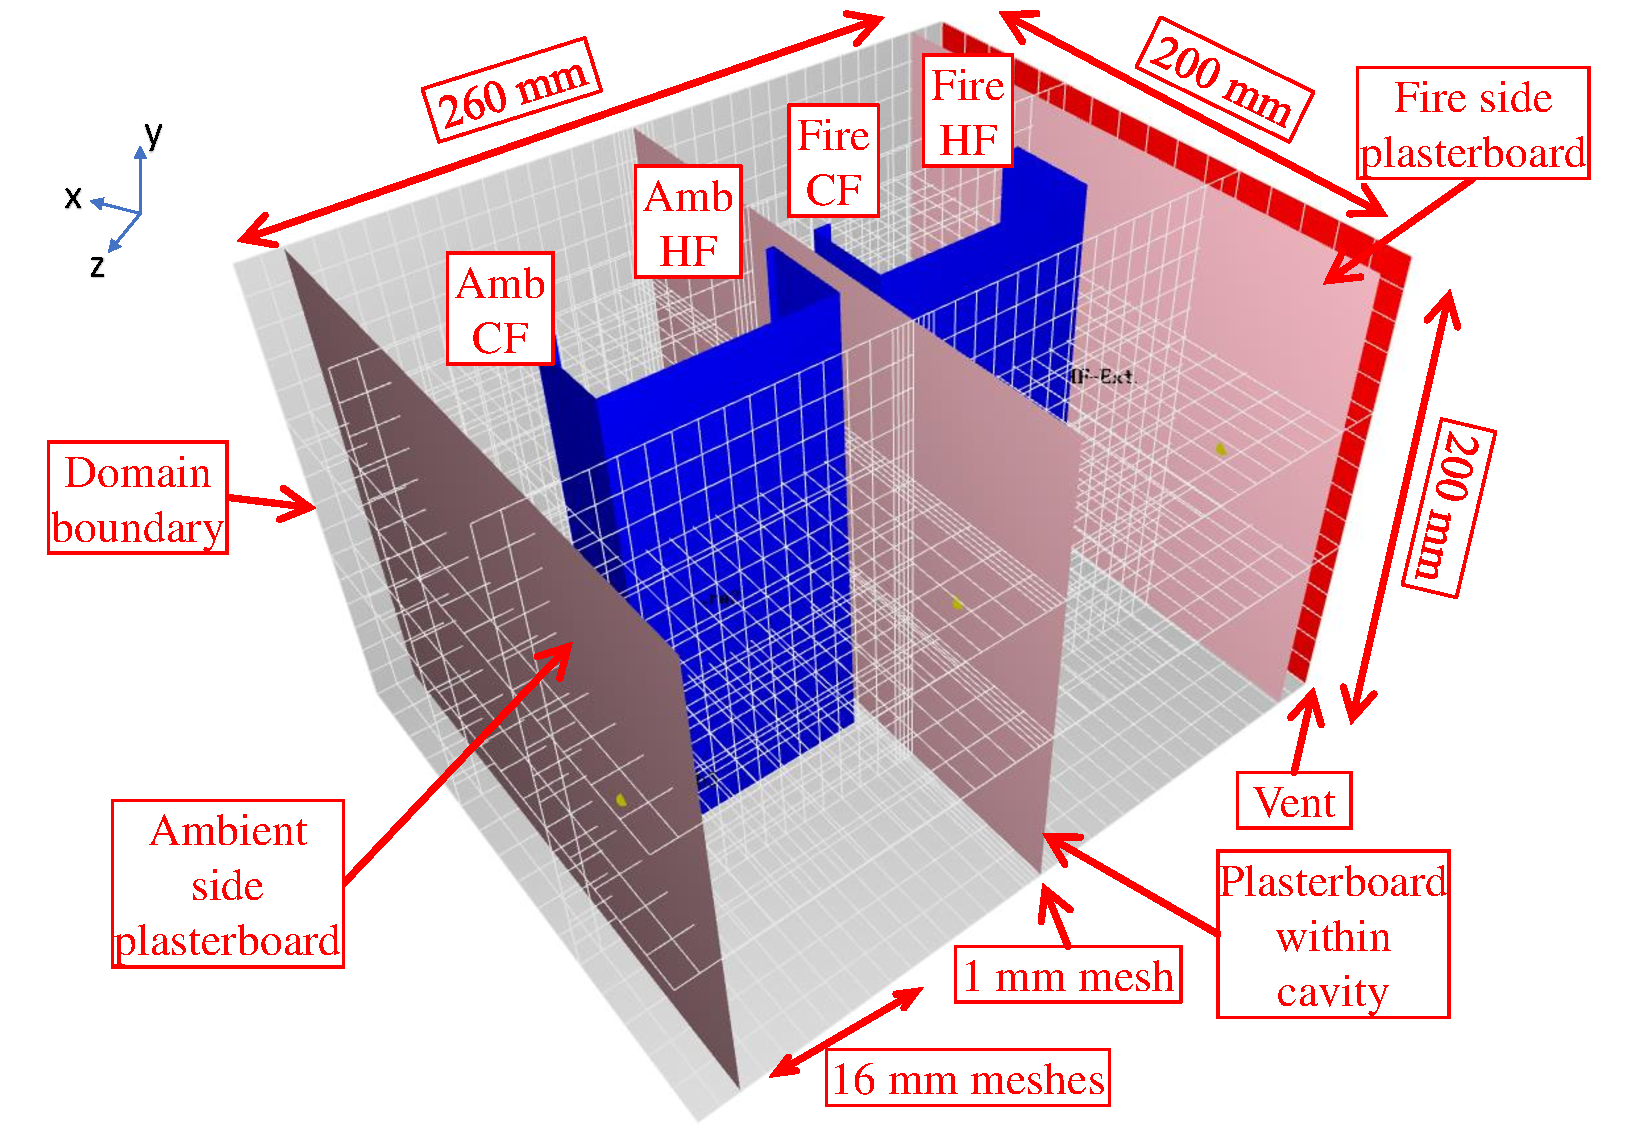
\includegraphics[scale=0.4]{T8-fds-model.pdf}
		\caption{Thermal model of Test-T8 wall}
		\label{fig:T8-fds-model}
\end{figure}
\begin{figure}[htbp]
	\centering
		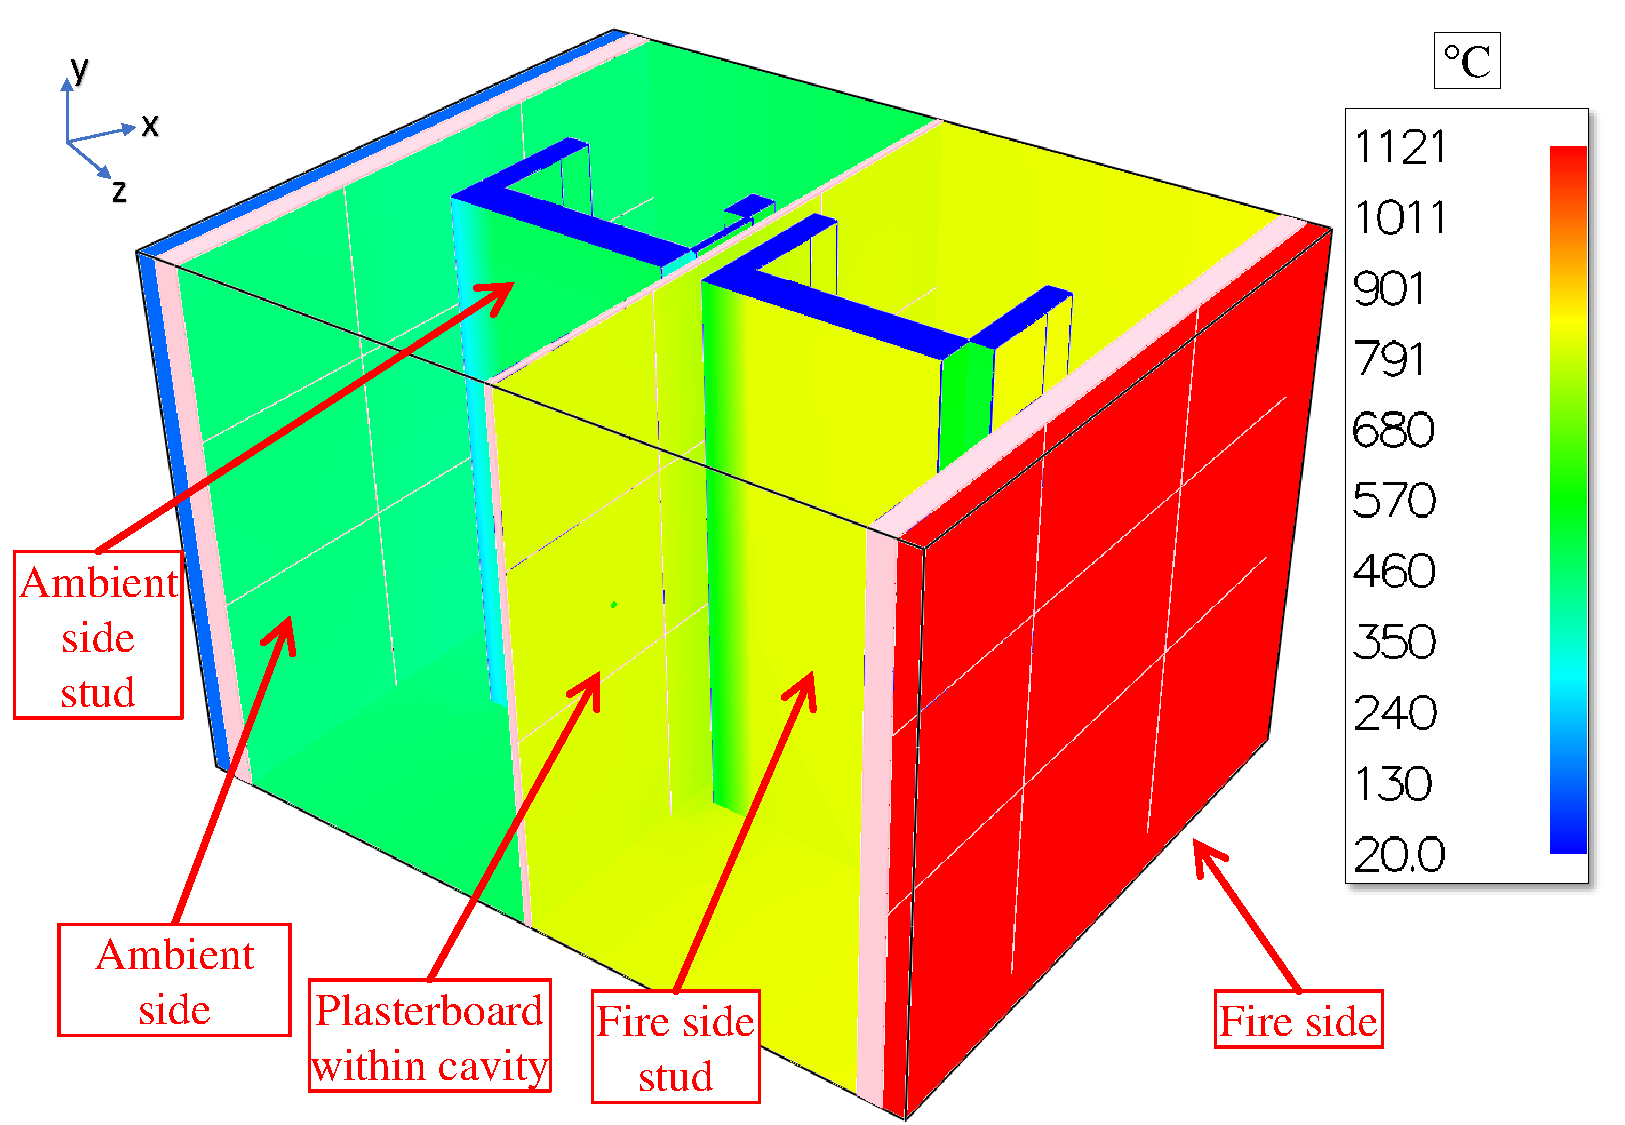
\includegraphics[scale=0.4]{T8-fds-output.pdf}
		\caption{Thermal model output from Test-T8 wall}
		\label{fig:T8-fds-output}
\end{figure}
\begin{figure}[!htbp]
	\centering
	\begin{subfigure}[b]{0.7\textwidth}
		\centering
		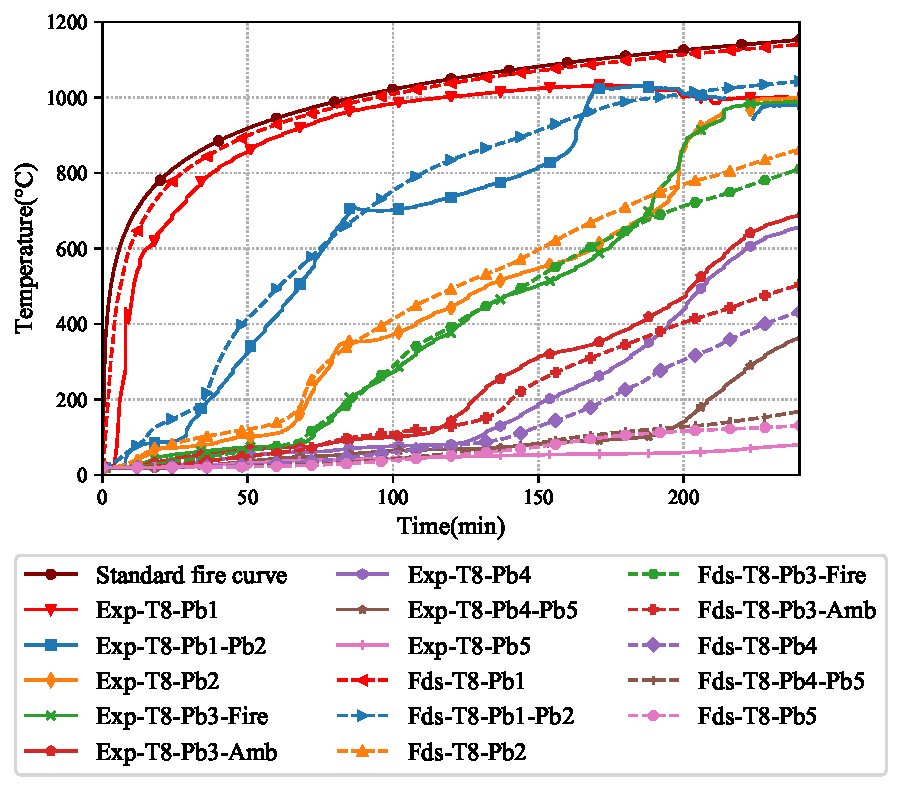
\includegraphics[width=\textwidth]{T8-r22-Pb-Fds-vs-Exp.pdf}
		\caption{}
		\label{subfig:T8-r22-Pb-Fds-vs-Exp}
	\end{subfigure}
	\begin{subfigure}[b]{0.6\textwidth}
		\centering
		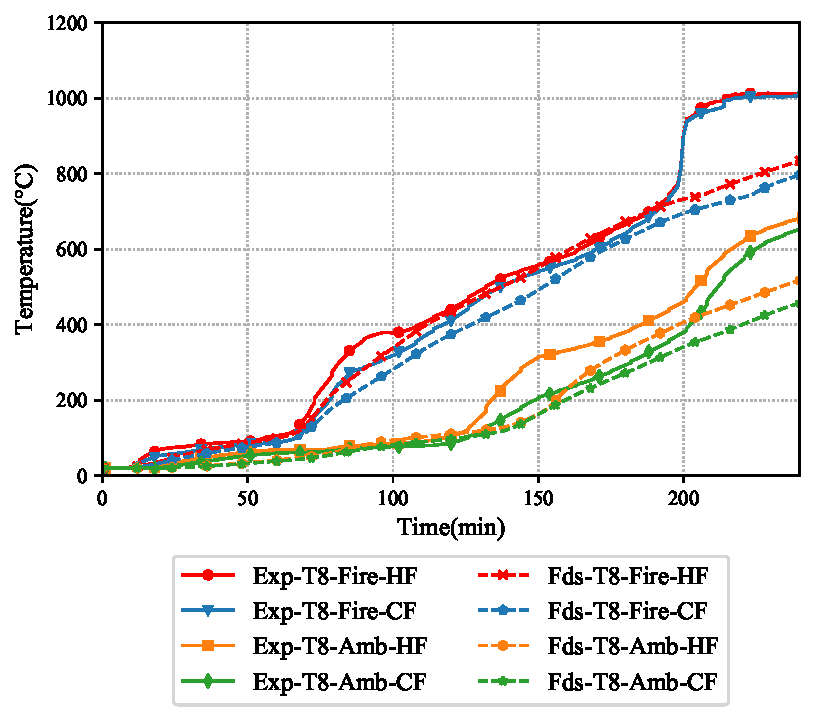
\includegraphics[width=\textwidth]{T8-r22-Studs-4-Fds-vs-Exp.pdf}
		\caption{}
		\label{subfig:T8-r22-Studs-4-Fds-vs-Exp}
	\end{subfigure}
	   \caption{Comparison of time-temperature curves from experiment and FDS model for Test-T8 (a) Average Plasterboard (b) Stud4-Mid}
	   \label{fig:fds-output-pb-studs-t8}
\end{figure}

Test-T8 was conducted on a shaftliner LSF wall where a plasterboard was placed within the cavity thereby splitting the cavity into two as shown in \Cref{fig:T8-fds-model}. The temperature profile from the FDS model are also shown in \Cref{fig:T8-fds-output}. \Cref{subfig:T8-r22-Pb-Fds-vs-Exp} compares the plasterboard time-temperature curves from FDS model and experiment for Test-T8. The time-temperature curves of the plasterboard from FDS thermal model match reasonably well with the experimental results till 160 min of the fire test. Due to the occurrence of significant plasterboard fall-off in the experiment, the resulting steep increase in the time-temperature curve near the end could not be simulated by the FDS thermal model. This was also reflected in the stud time-temperature curves shown in \Cref{subfig:T8-r22-Studs-4-Fds-vs-Exp}. The hot and cold flanges match reasonably well till the plasterboard fall-off time in the experiment.
\begin{figure}[!htbp]
	\centering
		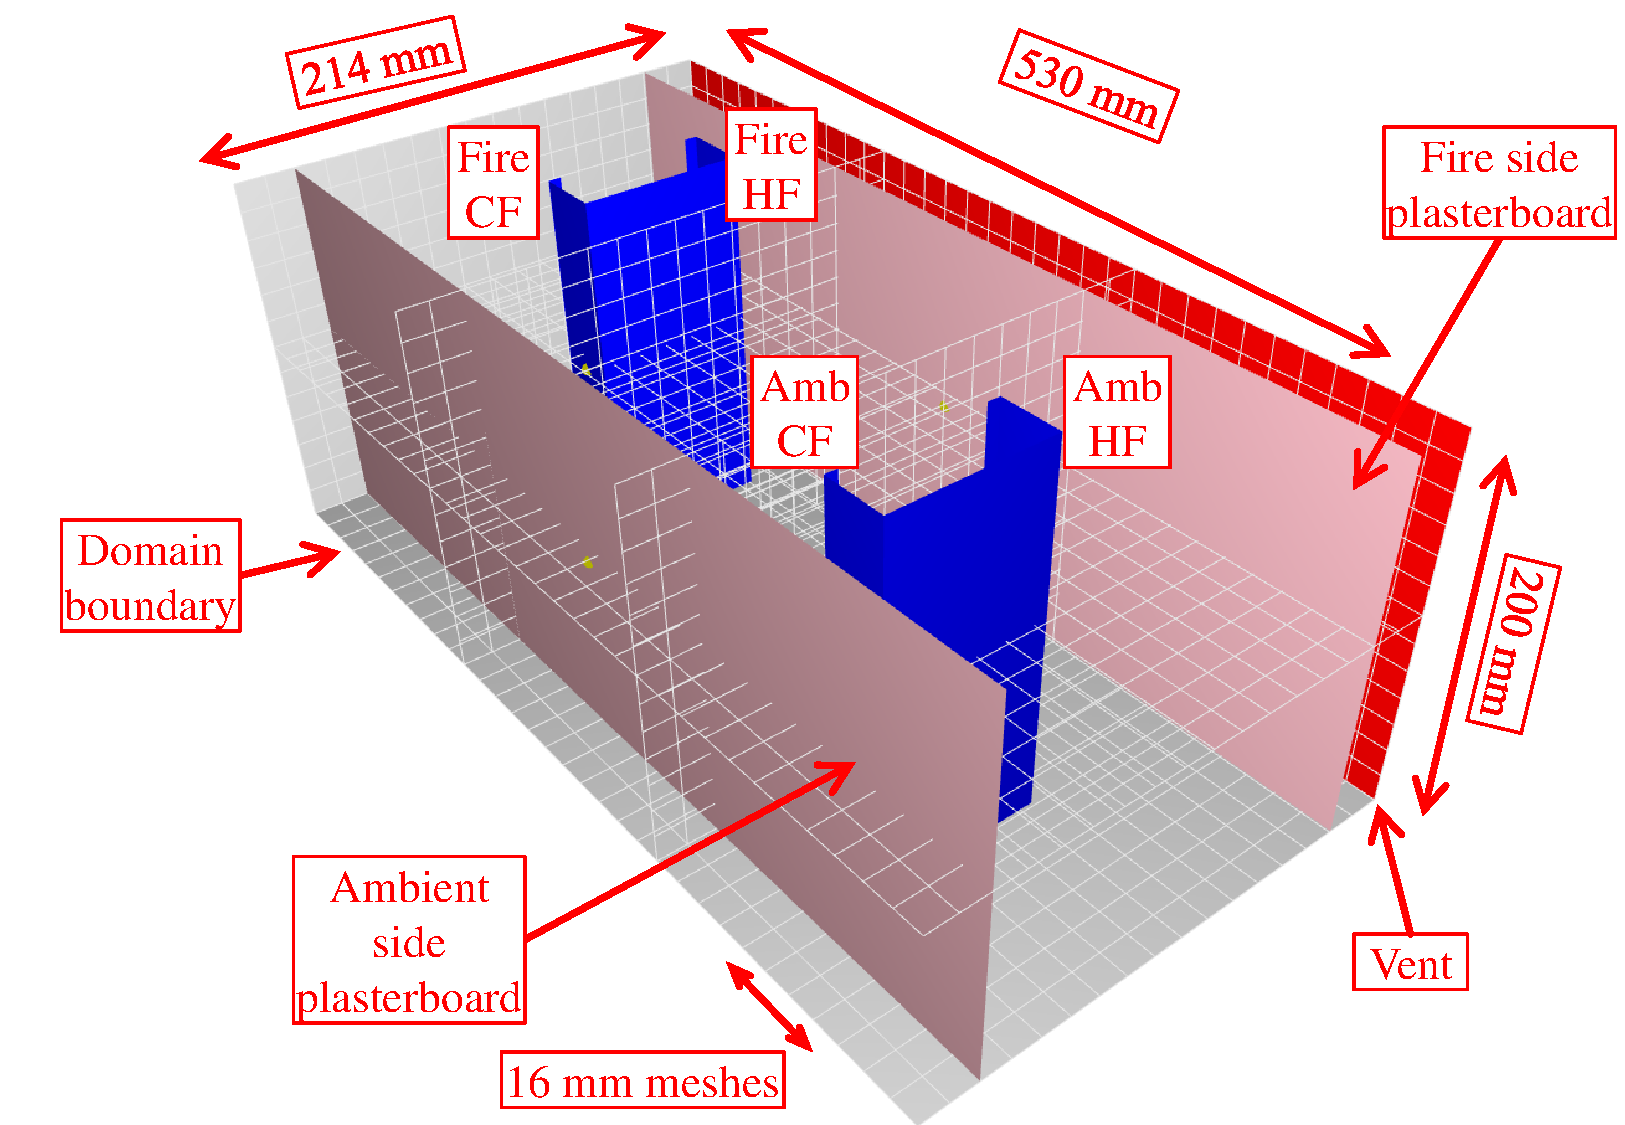
\includegraphics[scale=0.35]{T9-fds-model.pdf}
		\caption{Thermal model of Test-T9 wall}
		\label{fig:T9-fds-model}
\end{figure}
\begin{figure}[!htbp]
	\centering
		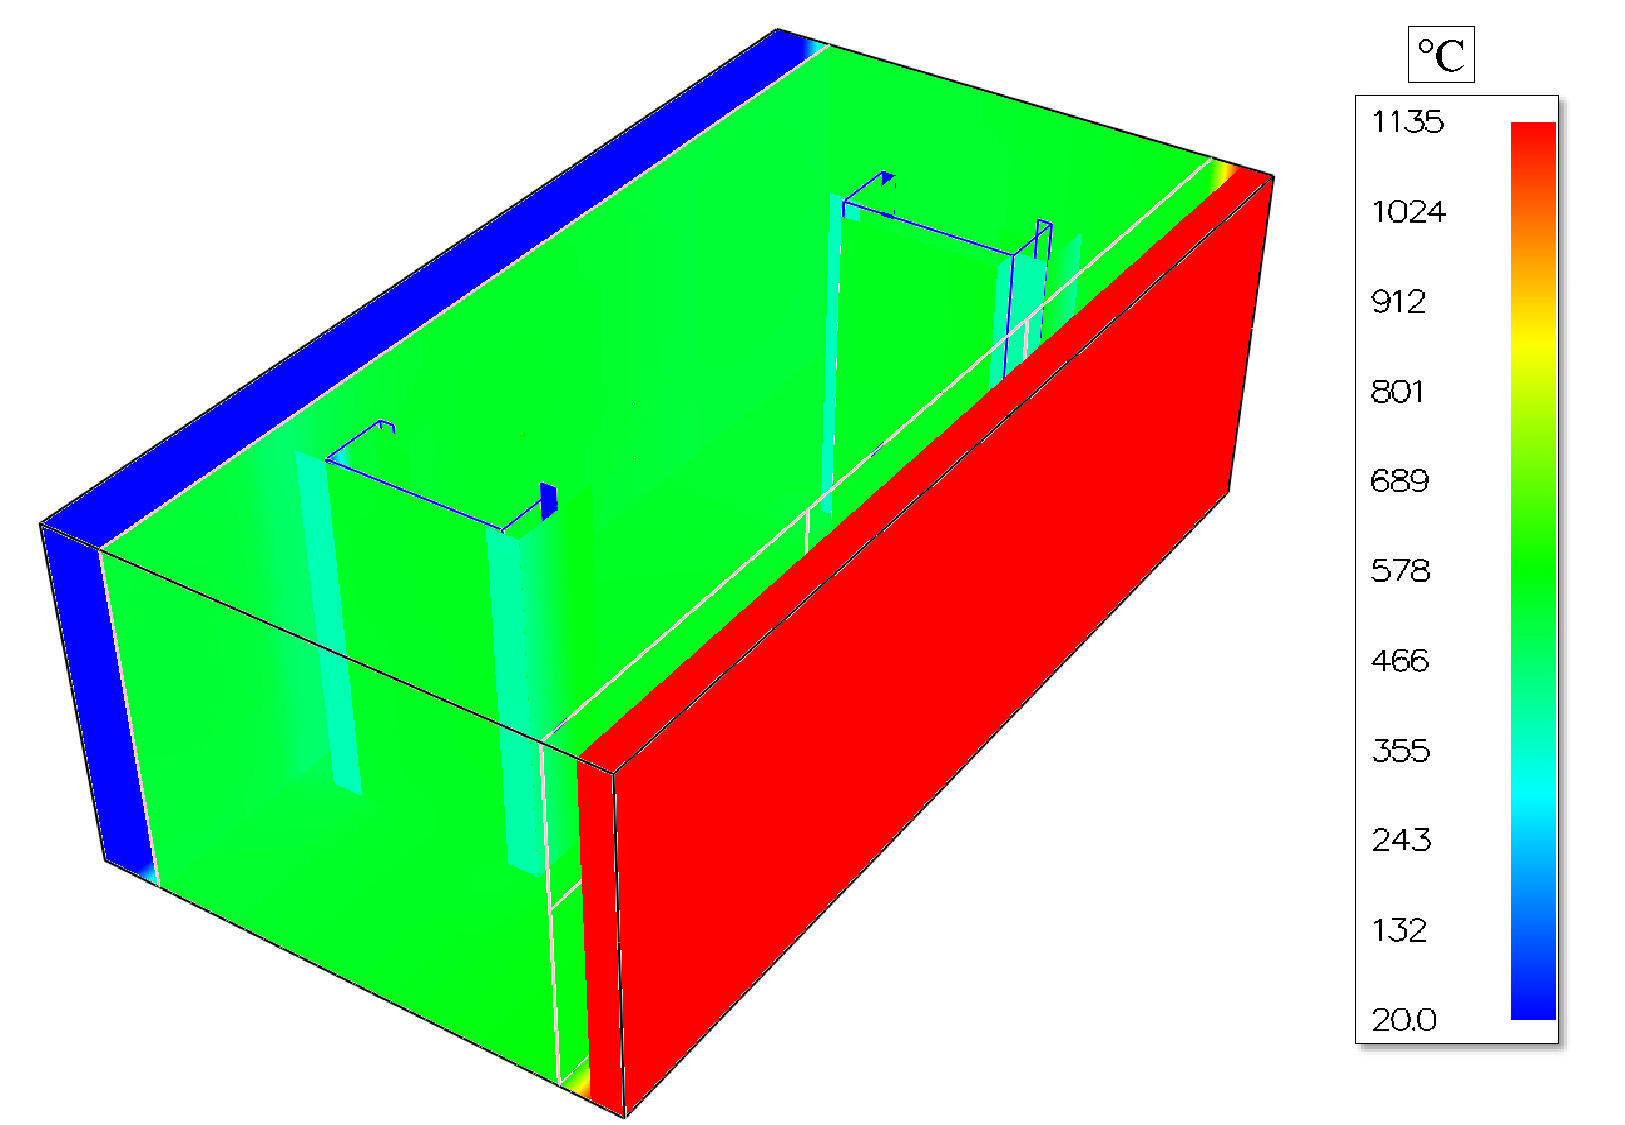
\includegraphics[scale=0.35]{T9-fds-output.pdf}
		\caption{Thermal model of Test-T9 wall}
		\label{fig:T9-fds-model}
\end{figure}
\begin{figure}[!htbp]
	\centering
	\begin{subfigure}[b]{0.7\textwidth}
		\centering
		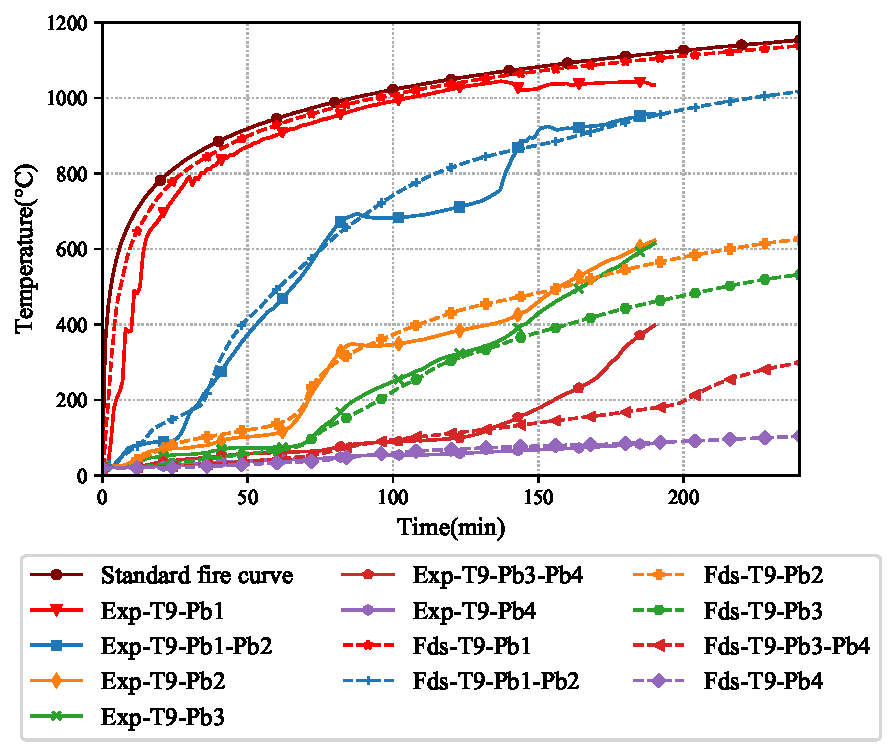
\includegraphics[width=\textwidth]{T9-r1-Pb-Fds-vs-Exp.pdf}
		\caption{}
		\label{subfig:T9-r1-Pb-Fds-vs-Exp}
	\end{subfigure}
	\begin{subfigure}[b]{0.6\textwidth}
		\centering
		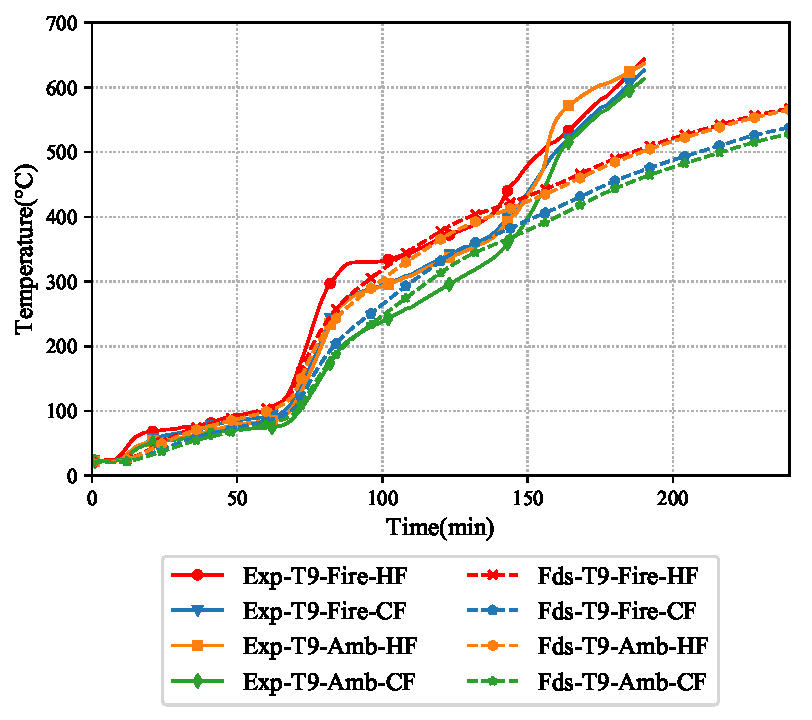
\includegraphics[width=\textwidth]{T9-r1-Studs-4-Fds-vs-Exp.pdf}
		\caption{}
		\label{subfig:T9-r1-Studs-4-Fds-vs-Exp}
	\end{subfigure}
	   \caption{Comparison of time-temperature curves from experiment and FDS model for Test-T9 (a) Average Plasterboard (b) Stud4-Mid}
	   \label{fig:fds-output-pb-studs-t9}
\end{figure}

Test-T9 was conducted on staggered stud LSF wall with a cavity depth of 150 mm. The studs in the test wall were arranged in a staggered manner wherein the hot flange of the ambient side stud does not have direct contact with the plasterboard. The plasterboard time-temperature curves from the experiment and FDS thermal model are compared in \Cref{subfig:T9-r1-Pb-Fds-vs-Exp}. A reasonable agreement is observed in the time-temperature curve comparison between the experiment and the FDS thermal model. The thermal model predictions were marginally above the experimental results till 120 min of the time-temperature curve. After 150 min significant plasterboard fall-off was observed in the fire Test-T9, which resulted in a higher time-temperature curve as shown in \Cref{subfig:T9-r1-Pb-Fds-vs-Exp}. This is also evident in the stud time-temperature curves as shown in \Cref{subfig:T9-r1-Studs-4-Fds-vs-Exp}. The stud time-temperature curves from the FDS thermal model were also in close agreement with the experimental results till 150 min. However, the FDS stud time-temperature curve exhibited a gradual rise after 150 min, while the experimental curves exhibited a steep rise. Ambient side hot flange facing the plasterboard recorded temperatures higher than the fire side cold flange in the experiments as this was close to the fire side plasterboard. This behaviour was also captured by the FDS thermal model. Based on the above-mentioned comparison it is evident that the FDS thermal model developed in this study can be used to predict thermal behaviour of non-cavity insulated complex LSF wall systems. 

\subsection{Thermal model validation - Cavity insulated Tests-T5, T6, T7 and T10}\label{sec:fds-cavity-models}

FDS model similar to the non-cavity insulated test wall was used to predict the time-temperature profile for cavity insulated test walls also. The use of cavity insulation was also achieved with ``1-cell thick" rule in FDS. The obstruction (\&OBST) for cavity insulation was modelled without intersecting with the other \&OBST such as plasterboard or stud to avoid numerical instability in the thermal model. FDS thermal model representing Test-T5 of a cavity insulated double stud wall made of 90 $\times$ 0.95 mm studs is shown in \Cref{fig:T5-fds-model-cavity}.
\begin{figure}[!htbp]
	\centering
		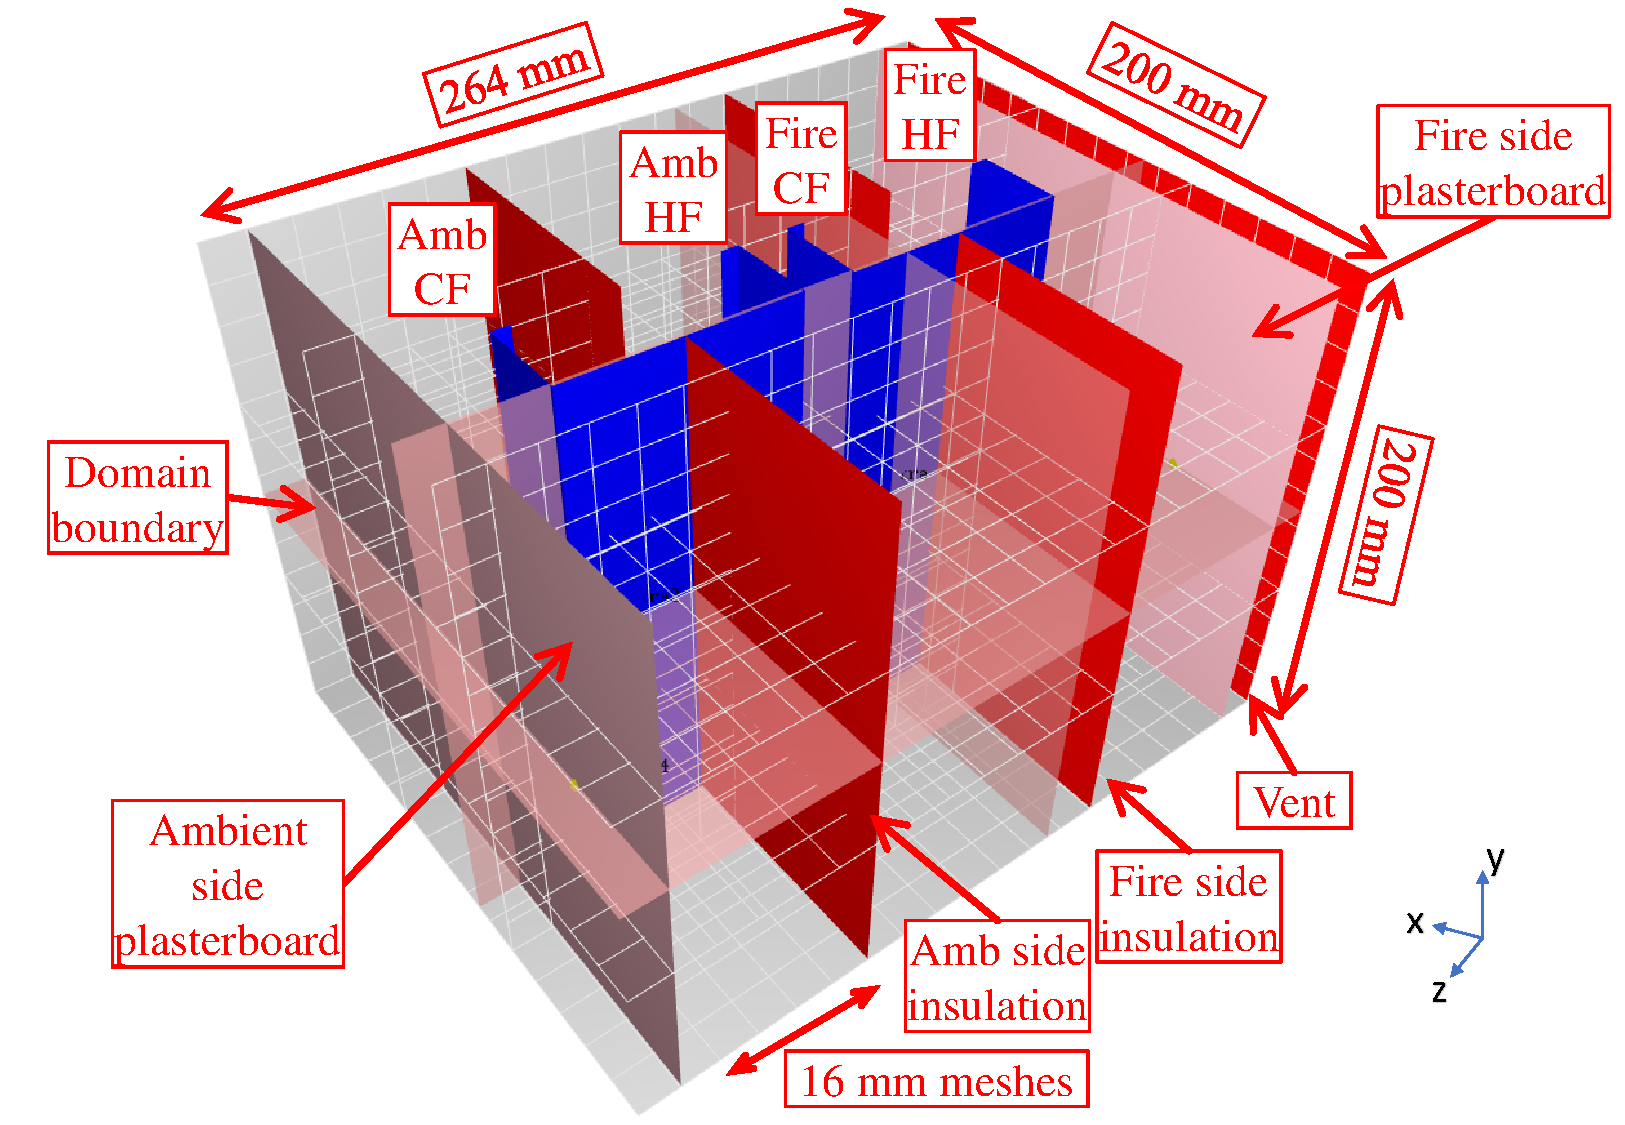
\includegraphics[width=10cm, height=8cm]{T5-fds-model.pdf}
		\caption{Thermal model of Test-T5 wall}
		\label{fig:T5-fds-model-cavity}
\end{figure}
\begin{figure}[!htbp]
	\centering
	\begin{subfigure}[b]{0.7\textwidth}
		\centering
		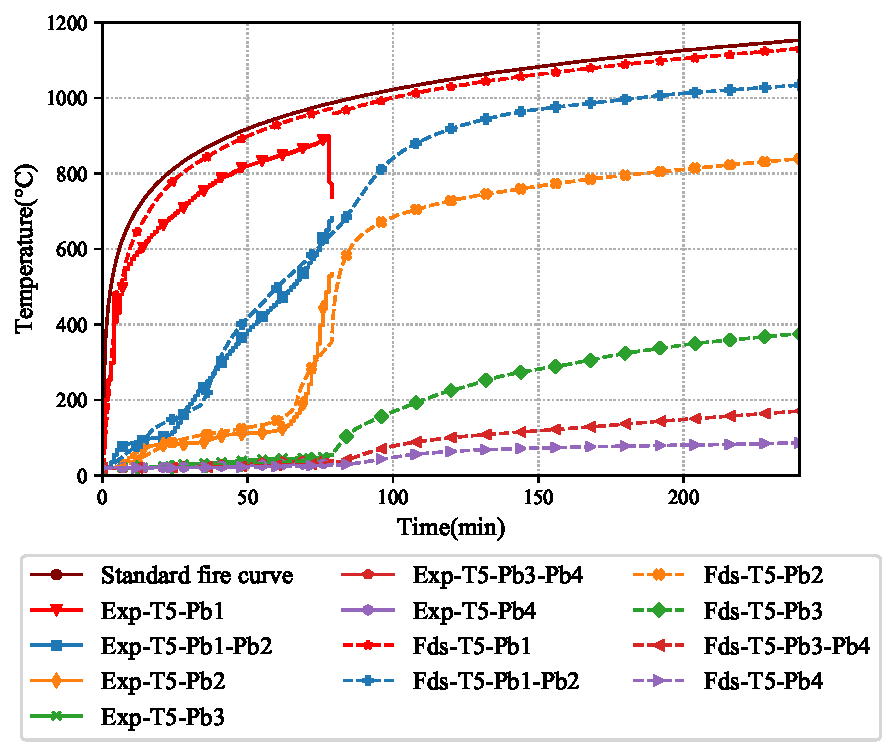
\includegraphics[width=\textwidth]{T5-r41-Pb-Fds-vs-Exp.pdf}
		\caption{}
		\label{subfig:T5-r41-Pb-Fds-vs-Exp}
	\end{subfigure}
	\begin{subfigure}[b]{0.6\textwidth}
		\centering
		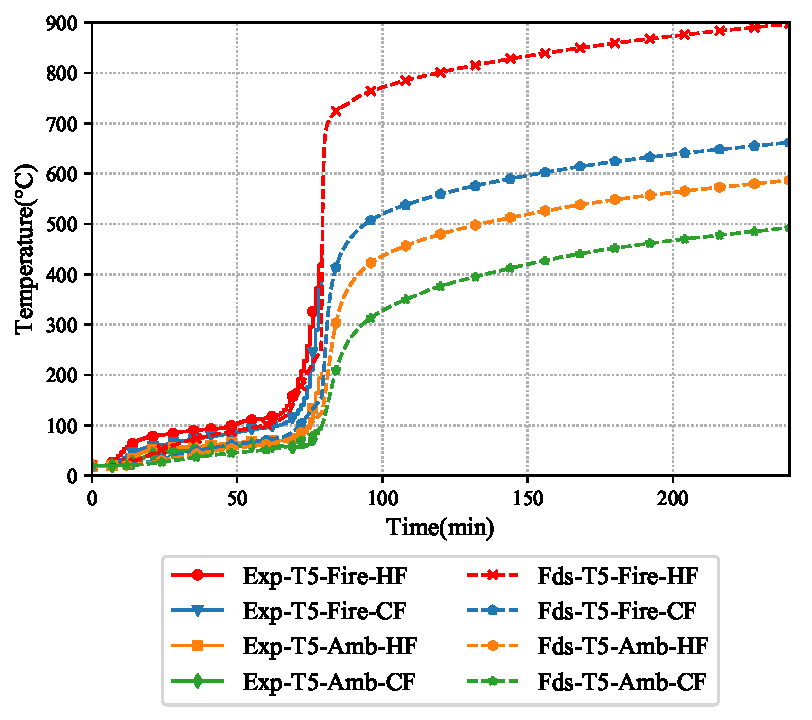
\includegraphics[width=\textwidth]{T5-r41-Studs-3-Fds-vs-Exp.pdf}
		\caption{}
		\label{subfig:T5-r41-Studs-3-Fds-vs-Exp}
	\end{subfigure}
	   \caption{Comparison of time-temperature curves from experiment and FDS model for Test-T5 (a) Average Plasterboard (b) Stud3-Mid}
	   \label{fig:fds-output-pb-studs-t5}
\end{figure}

\Cref{subfig:T5-r41-Pb-Fds-vs-Exp} compares the plasterboard time-temperature curves from FDS thermal model and experiment. An important observation in the case of cavity insulated wall is the sudden increase of the fire side cavity time-temperature curve (Exp-T5-Pb2). This indicates the presence of severe plasterboard open up and was also reported in \Cref{ch:Fire}. Plasterboard open-up occurs predominantly in the plasterboard joints or in the weakest portion of the test wall. However, in the present model the plasterboard open-up is considered by removing the middle portion as shown in \Cref{subfig:T5-fds-at-openup} to all the models for simplification. To achieve the plasterboard open-up effect on FDS thermal model, the concept of ``set-point'' temperature was used in the fire side plasterboard interface (Pb1-Pb2). Once the thermocouple Pb1-Pb2 reaches the set point temperature a portion of the plasterboard was removed during the analysis and the thermal analysis was continued till 240 min with a hole in the fire side plasterboard as shown \Cref{fig:T5-fds-output}. A ``set-point'' temperature of 640\degree C was used at the plasterboard interface (Pb1-Pb2) to initiate the plasterboard open-up based on based on ASTM 1588 (\citet{Sultan2015}). 
\begin{figure}[!htbp]
	\centering
	\begin{subfigure}[b]{0.45\textwidth}
		\centering
		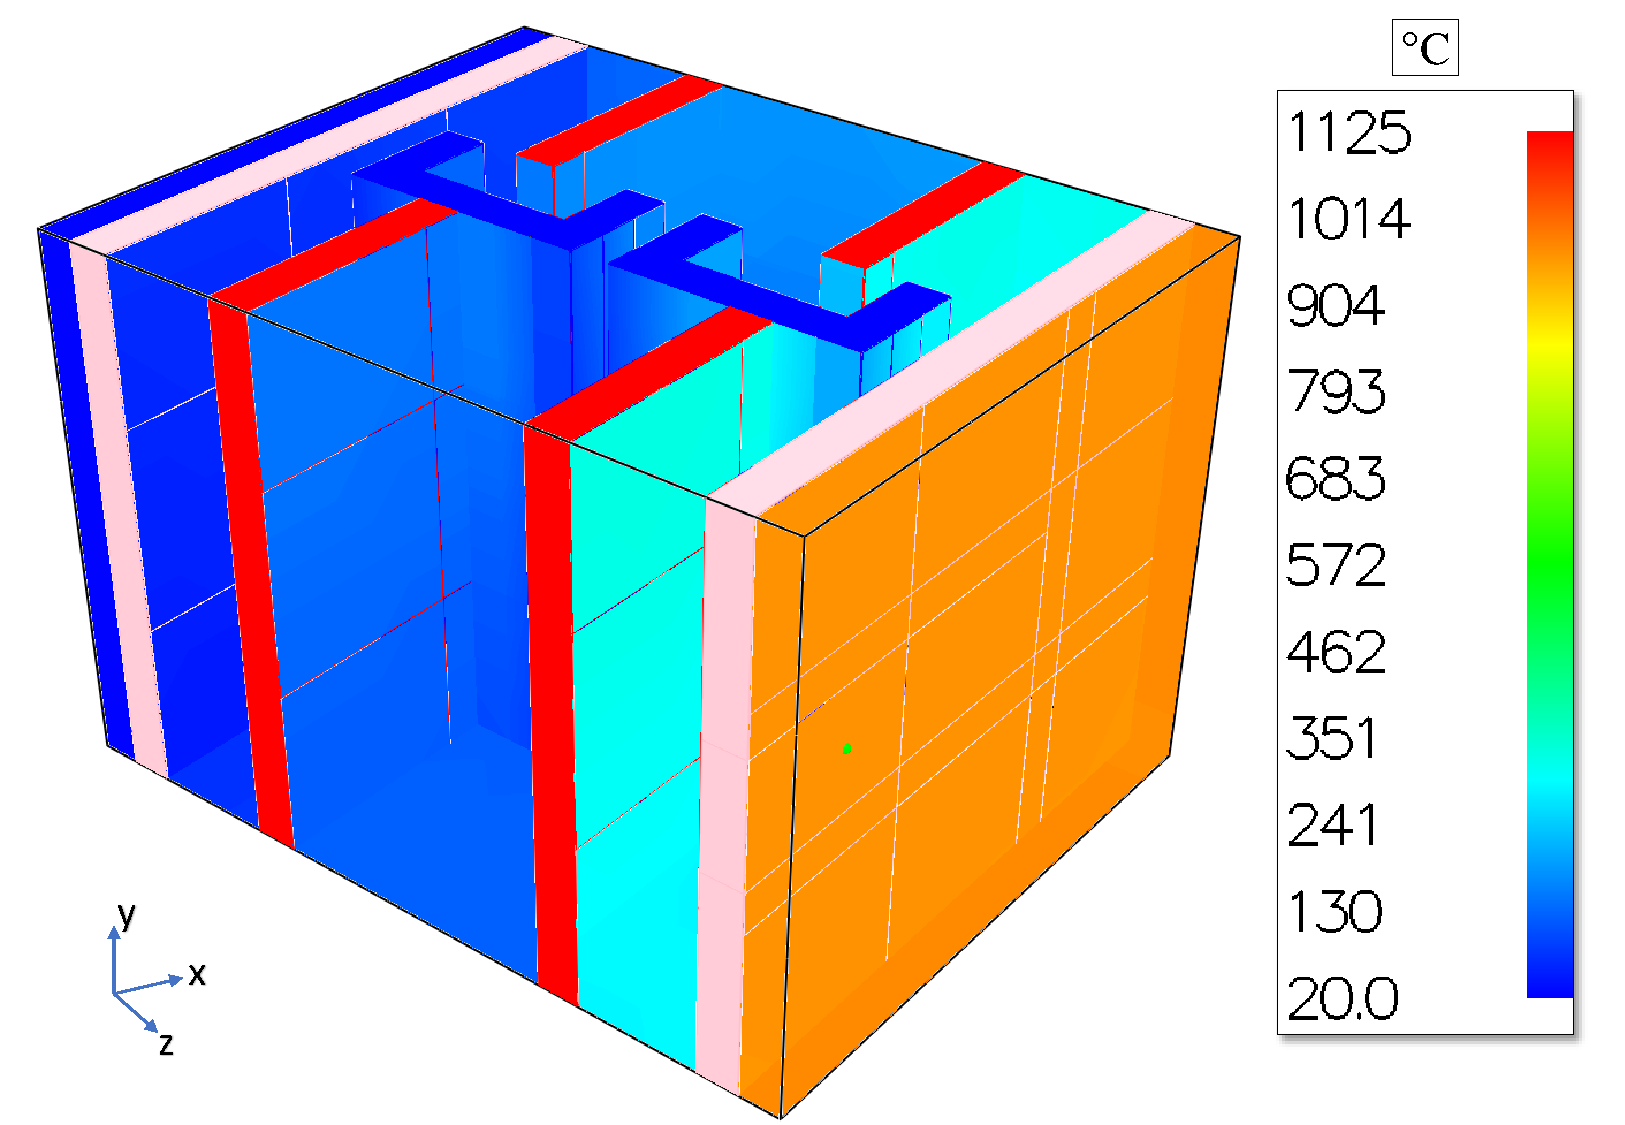
\includegraphics[width=\textwidth]{T5-fds-before-openup.pdf}
		\caption{}
		\label{subfig:T5-fds-before-openup}
	\end{subfigure}
	\begin{subfigure}[b]{0.45\textwidth}
		\centering
		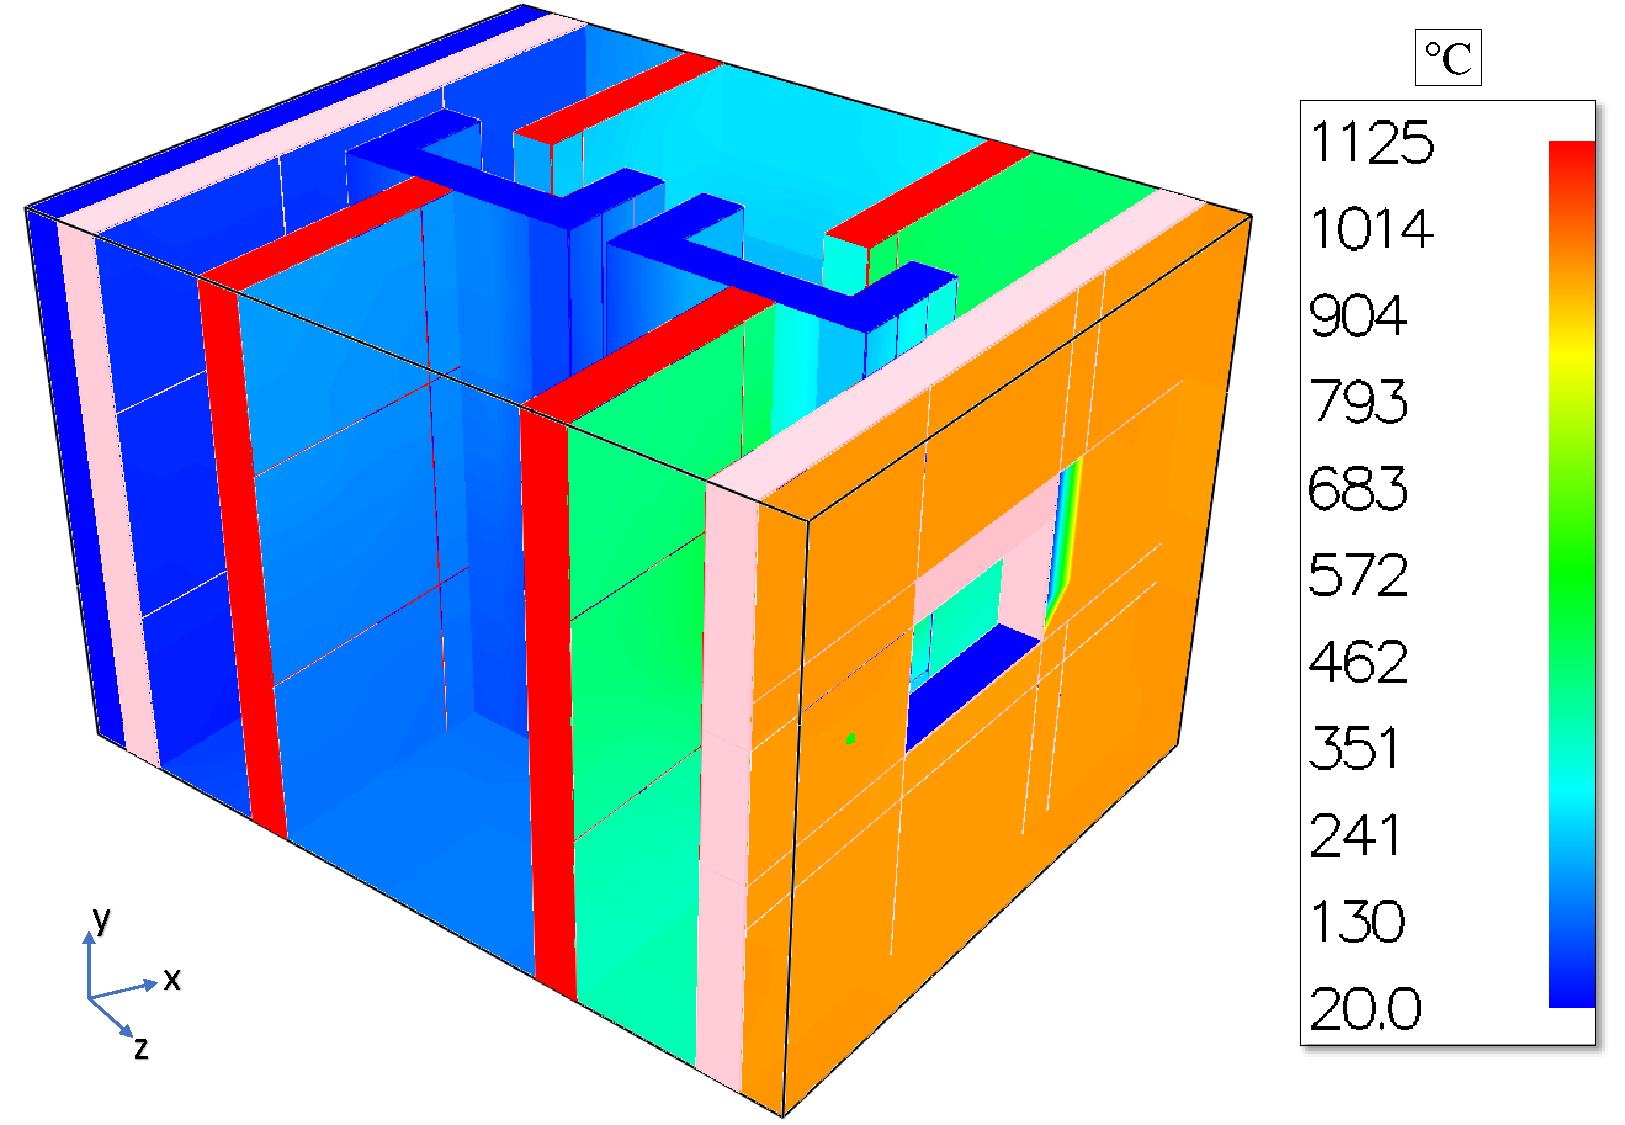
\includegraphics[width=\textwidth]{T5-fds-at-openup.pdf}
		\caption{}
		\label{subfig:T5-fds-at-openup}
	\end{subfigure}
	\begin{subfigure}[b]{0.45\textwidth}
		\centering
		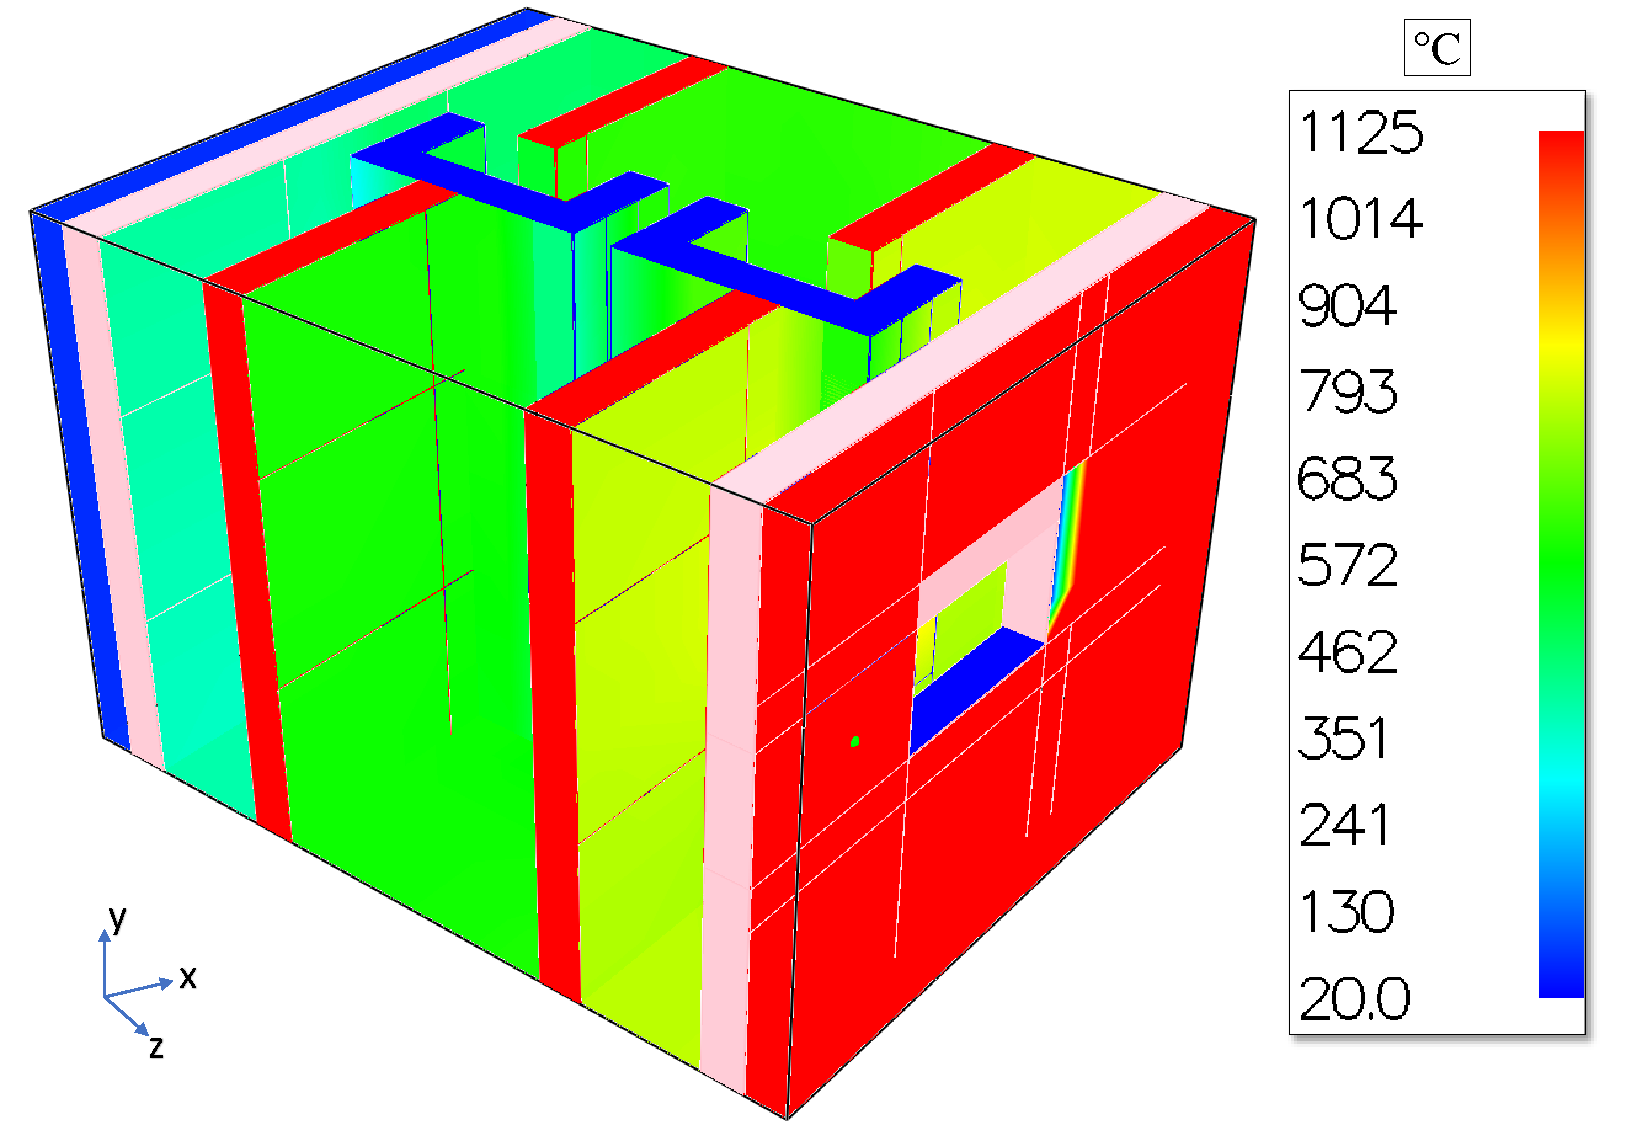
\includegraphics[width=\textwidth]{T5-fds-end-openup.pdf}
		\caption{}
		\label{subfig:T5-fds-end-openup}
	\end{subfigure}
	   \caption{Temperature profile of Test-T5 from FDS thermal analysis (a) Before plasterboard open-up at 78 min (b) After plasterboard open-up at 79 min (c) At 240 min (End of Simulation)}
	   \label{fig:T5-fds-output}
\end{figure}
\begin{figure}[!htbp]
	\centering
	\begin{subfigure}[b]{0.7\textwidth}
		\centering
		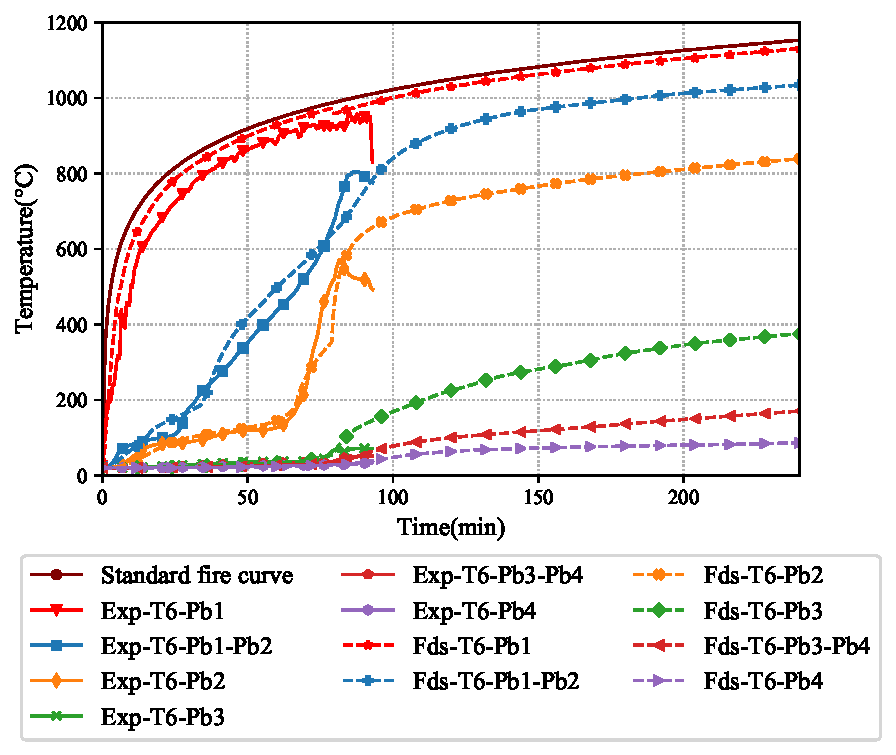
\includegraphics[width=\textwidth]{T6-r7-Pb-Fds-vs-Exp.pdf}
		\caption{}
		\label{subfig:T6-r7-Pb-Fds-vs-Exp}
	\end{subfigure}
	\begin{subfigure}[b]{0.6\textwidth}
		\centering
		\includegraphics[width=\textwidth]{T6-r7-Studs-4-Fds-vs-Exp.pdf}
		\caption{}
		\label{subfig:T6-r7-Studs-4-Fds-vs-Exp}
	\end{subfigure}
	   \caption{Comparison of time-temperature curves from experiment and FDS model for Test-T6 (a) Average Plasterboard (b) Stud4-Mid}
	   \label{fig:fds-output-pb-studs-t6}
\end{figure}

The FDS thermal model was able to simulate the steep rise in time-temperature curve experienced in thermocouple Exp-T5-Pb2 as shown in \Cref{subfig:T5-r41-Pb-Fds-vs-Exp} to a reasonable accuracy and was also able to predict the temperature profile till 240 min. Reasonable agreement was observed on all the plasterboard time-temperature curves. Stud time-temperature curves shown in \Cref{subfig:T5-r41-Studs-3-Fds-vs-Exp} also exhibited good agreement with the experimental results. Test-T6 was conducted as a repeat test and the corresponding model validation for time-temperature curves are shown in Figures \ref{fig:fds-output-pb-studs-t6} (a) and (b). Time-temperature curve agreement between FDS thermal model and the experimental results is good for Test-T6 also.
\begin{figure}[!htbp]
	\centering
		\includegraphics[width=9cm, height=6cm]{T7-fds-model.pdf}
		\caption{Thermal model of Test-T7 wall}
		\label{fig:T7-fds-model-cavity}
\end{figure}
\begin{figure}[!htbp]
	\centering
	\begin{subfigure}[b]{0.45\textwidth}
		\centering
		\includegraphics[width=\textwidth]{T7-fds-before-openup.pdf}
		\caption{}
		\label{subfig:T7-fds-before-openup}
	\end{subfigure}
	\begin{subfigure}[b]{0.45\textwidth}
		\centering
		\includegraphics[width=\textwidth]{T7-fds-at-openup.pdf}
		\caption{}
		\label{subfig:T7-fds-at-openup}
	\end{subfigure}
	\begin{subfigure}[b]{0.45\textwidth}
		\centering
		\includegraphics[width=\textwidth]{T7-fds-end-openup.pdf}
		\caption{}
		\label{subfig:T7-fds-end-openup}
	\end{subfigure}
	   \caption{Temperature profile of Test-T7 from FDS thermal analysis (a) Before plasterboard open-up at 79 min (b) After plasterboard open-up at 80 min (c) At 240 min (End of Simulation)}
	   \label{fig:T7-fds-output}
\end{figure}
\begin{figure}[!htbp]
	\centering
	\begin{subfigure}[b]{0.7\textwidth}
		\centering
		\includegraphics[width=\textwidth]{T7-r7-Pb-Fds-vs-Exp.pdf}
		\caption{}
		\label{subfig:T7-r7-Pb-Fds-vs-Exp}
	\end{subfigure}
	\begin{subfigure}[b]{0.6\textwidth}
		\centering
		\includegraphics[width=\textwidth]{T7-r7-Studs-3-Fds-vs-Exp.pdf}
		\caption{}
		\label{subfig:T7-r7-Studs-3-Fds-vs-Exp}
	\end{subfigure}
	   \caption{Comparison of time-temperature curves from experiment and FDS model for Test-T7 (a) Average Plasterboard (b) Stud3-Mid}
	   \label{fig:fds-output-pb-studs-t7}
\end{figure}

Test-T7 was conducted on double stud LSF wall with 90 $\times$ 0.95 mm studs wherein the cavity insulation was placed only within the ambient side row of studs (0.4 Load Ratio). \Cref{fig:T7-fds-model-cavity} shows the FDS model with ambient side cavity insulation considered for the thermal analysis. \Cref{subfig:T7-r7-Pb-Fds-vs-Exp}compares the time-temperature curves from FDS thermal analysis and experiment. Sudden increase in the plasterboard time-temperature curve (Exp-T7-Pb2) was observed in this fire test also. This behaviour was also predicted by the developed FDS thermal model and is evident from the comparison in \Cref{fig:fds-output-pb-studs-t7} (a). Increase in the plasterboard time-temperature curves also affects the corresponding stud hot and cold flange temperatures. The developed FDS thermal model was able to predict the sudden increase in the stud hot and cold flange time-temperature curves as shown in \Cref{fig:fds-output-pb-studs-t7} (b) with a reasonable agreement. 
\begin{figure}[!htbp]
	\centering
		\includegraphics[width=9cm, height=6cm]{T10-fds-model.pdf}
		\caption{Thermal model of Test-T10 wall}
		\label{fig:T10-fds-model-cavity}
\end{figure}

Cavity insulated staggered stud wall Test-T10 made of 90 $\times$ 0.95 mm studs (0.4 Load Ratio) was modelled as shown in \Cref{fig:T10-fds-model-cavity}. Cavity insulation was curved through the studs in the test wall. However, to increase the computational efficiency the cavity insulation is staggered linearly between the studs with two horizontal and one vertical obstruction (\&OBST) as shown in \Cref{fig:T10-fds-model-cavity}. Time-temperature curves from FDS thermal model are compared against experimental results in Figures \ref{fig:fds-output-pb-studs-t10} (a) and (b).
\begin{figure}[!htbp]
	\centering
	\begin{subfigure}[b]{0.45\textwidth}
		\centering
		\includegraphics[width=\textwidth]{T10-fds-before-openup.pdf}
		\caption{}
		\label{subfig:T10-fds-before-openup}
	\end{subfigure}
	\begin{subfigure}[b]{0.45\textwidth}
		\centering
		\includegraphics[width=\textwidth]{T10-fds-at-openup.pdf}
		\caption{}
		\label{subfig:T10-fds-at-openup}
	\end{subfigure}
	\begin{subfigure}[b]{0.45\textwidth}
		\centering
		\includegraphics[width=\textwidth]{T10-fds-end-openup.pdf}
		\caption{}
		\label{subfig:T10-fds-end-openup}
	\end{subfigure}
	   \caption{Temperature profile of Test-T10 from FDS thermal analysis (a) Before plasterboard open-up at 79 min (b) After plasterboard open-up at 80 min (c) At 240 min (End of Simulation)}
	   \label{fig:T10-fds-output}
\end{figure}
\begin{figure}[!htbp]
	\centering
	\begin{subfigure}[b]{0.7\textwidth}
		\centering
		\includegraphics[width=\textwidth]{T10-r1-Pb-Fds-vs-Exp.pdf}
		\caption{}
		\label{subfig:T10-r1-Pb-Fds-vs-Exp}
	\end{subfigure}
	\begin{subfigure}[b]{0.6\textwidth}
		\centering
		\includegraphics[width=\textwidth]{T10-r1-Studs-4-Fds-vs-Exp.pdf}
		\caption{}
		\label{subfig:T10-r1-Studs-4-Fds-vs-Exp}
	\end{subfigure}
	   \caption{Comparison of time-temperature curves from experiment and FDS model for Test-T10 (a) Average Plasterboard (b) Stud3-Mid}
	   \label{fig:fds-output-pb-studs-t10}
\end{figure}

Plasterboard open-up was observed in the full-scale fire Test-T10 leading to the sudden temperature rise in the fire side cavity plasterboard surface (Exp-T10-Pb2) similar to other test walls with cavity insulation. The developed FDS thermal model was able to predict this behaviour to a reasonable accuracy for both plasterboard and stud time-temperature curves as shown in \Cref{fig:T10-fds-output}. Fire side plasterboard time-temperature curves matched reasonably well with the experimental results as shown in \Cref{subfig:T10-r1-Pb-Fds-vs-Exp}. However, the ambient side plasterboard temperatures were lower than the experimental results. This was observed for the stud hot and cold flanges as well. The fire side hot and cold flange temperatures (Fds-T10-Fire-HF and CF) matched reasonably well with the experiments as shown in \Cref{subfig:T10-r1-Studs-4-Fds-vs-Exp}. However, the ambient side hot and cold flange temperatures (Fds-T10-Amb-HF and CF) were lower than the experimental results. The increase in slope of the time-temperature curves on the ambient side hot and cold flanges occurred at a later time period in comparison with the experiments. This may lead to unconservative results in the structural model. 

\subsection{Thermal model validation - Non-cavity insulated Tests-T1, T2, T3, T4, T8 and T9 with plasterboard open-up} \label{sec:thermal-model-non-cav}

As the plasterboard open-up in fire tests contributes significantly to the time-temperature curves prediction, the non-cavity insulated test models were also analysed with the plasterboard openings in them. Similar technique used for cavity insulated wall tests as described in \Cref{sec:fds-cavity-models} were used for the developed thermal models. The set-point temperature was increased to 900\degree C for non-cavity insulated LSF walls based on \citet{Sultan2015}. The plasterboard open-up temperatures corresponding to the fire tests also match this assumption of 900\degree C in all the conducted non-cavity insulated fire tests. Determining the plasterboard open-up and predicting the corresponding stud hot flange temperatures is important, as these temperatures will be used in the structural FE model. The time-temperature curves from FDS thermal analysis pertaining to the tested wall configurations are presented and discussed next.

\begin{figure}[!htbp]
	\centering
	\begin{subfigure}[b]{0.6\textwidth}
		\centering
		\includegraphics[width=\textwidth]{T1-r63-Pb-Fds-vs-Exp.pdf}
		\caption{}
		\label{subfig:T1-r63-Pb-Fds-vs-Exp}
	\end{subfigure}
	\begin{subfigure}[b]{0.6\textwidth}
		\centering
		\includegraphics[width=\textwidth]{T1-r63-Studs-4-Fds-vs-Exp.pdf}
		\caption{}
		\label{subfig:T1-r63-Studs-4-Fds-vs-Exp}
	\end{subfigure}
	   \caption{Comparison of time-temperature curves from experiment and FDS model with plasterboard open-up for Test-T1 (a) Average Plasterboard (b) Stud4-Mid}
	   \label{fig:T1-fds-output-pbop}
\end{figure}

\Cref{fig:T1-fds-output-pbop} shows the plasterboard and stud time-temperature curves from FDS thermal model with plasterboard open-up for double stud wall Test-T1. The sudden increase in the plasterboard time-temperature curve at 176 min can be simulated reasonably as shown in \Cref{subfig:T1-r63-Pb-Fds-vs-Exp}. This sudden increase is also noticeable in the stud time-temperature curves comparison shown in \Cref{subfig:T1-r63-Studs-4-Fds-vs-Exp}. The fire side hot flange temperatures also agree reasonably well with the experimental results which will be used in the structural FE model for predicting the failure time of the wall configuration.

\begin{figure}[!htbp]
	\centering
	\begin{subfigure}[b]{0.7\textwidth}
		\centering
		\includegraphics[width=\textwidth]{T2-r1-Pb-Fds-vs-Exp.pdf}
		\caption{}
		\label{subfig:T2-r1-Pb-Fds-vs-Exp}
	\end{subfigure}
	\begin{subfigure}[b]{0.6\textwidth}
		\centering
		\includegraphics[width=\textwidth]{T2-r1-Studs-3-Fds-vs-Exp.pdf}
		\caption{}
		\label{subfig:T2-r1-Studs-3-Fds-vs-Exp}
	\end{subfigure}
	   \caption{Comparison of time-temperature curves from experiment and FDS model with plasterboard open-up for Test-T2 (a) Average Plasterboard (b) Stud4-Mid}
	   \label{fig:T2-fds-output-pbop}
\end{figure}

\Cref{fig:T2-fds-output-pbop} shows the time-temperature curve comparison for Test-T2. The sudden increase in the plasterboard time-temperature curve as shown in \Cref{subfig:T2-r1-Pb-Fds-vs-Exp} was noticeable from 120 min. However, the FDS thermal model predictions shows the sudden increase after 175 min. This is reflected in the stud time-temperature curves also as shown in \Cref{subfig:T2-r1-Studs-3-Fds-vs-Exp}. The delay in sudden temperature rise in the hot flange may lead to increased structural failure time which may lead to unconservative results. Test-T2 was conducted with 0.75 mm thick studs unlike Test-T1 with 0.95 mm studs. The set-point temperature of 900\degree may be higher for thinner stud section as Tests-T2 and T3 had higher lateral deflection in comparison with Tests-T1 and T4. This was because of the use of thinner studs in the test wall. Severe plasterboard fall-off was also observed in Test-T2 causing premature failure and was discussed in \Cref{sec:t2-fire-test} of \Cref{ch:Fire}. However, this will further be discussed in \Cref{ch:FE-Structural}. Also, during fire tests under load bearing conditions, the furnace is stopped once the test wall fails due to structural inadequacy criteria on the time-temperature curves of plasterboard and studs dips after this time and is evident by the cooling face of the time-temperature curves as shown in \Cref{fig:T2-fds-output-pbop}. However, the FDS models are analysed for a time period of 240 min. The behaviour of the test wall post fire test can be determined through this which will help in determining the structural failure time of the test wall under different load ratios. As Test-T3 was conducted with the same configuration as Test-T2 under a higher load ratio (0.6 LR) the time-temperature curves from the experimental results are available only till 81 min. Comparison of the time-temperature curves of the plasterboards and studs are shown in \Cref{fig:T3-fds-output-pbop}, but will not be considered for detailed discussion.  

\begin{figure}[!htbp]
	\centering
	\begin{subfigure}[b]{0.7\textwidth}
		\centering
		\includegraphics[width=\textwidth]{T3-r1-Pb-Fds-vs-Exp.pdf}
		\caption{}
		\label{subfig:T3-r1-Pb-Fds-vs-Exp}
	\end{subfigure}
	\begin{subfigure}[b]{0.6\textwidth}
		\centering
		\includegraphics[width=\textwidth]{T3-r1-Studs-4-Fds-vs-Exp.pdf}
		\caption{}
		\label{subfig:T3-r0-Studs-4-Fds-vs-Exp}
	\end{subfigure}
	   \caption{Comparison of time-temperature curves from experiment and FDS model with plasterboard open-up for Test-T3 (a) Average Plasterboard (b) Stud4-Mid}
	   \label{fig:T3-fds-output-pbop}
\end{figure}
\begin{figure}[!htbp]
	\centering
	\begin{subfigure}[b]{0.7\textwidth}
		\centering
		\includegraphics[width=\textwidth]{T4-r4-Pb-Fds-vs-Exp.pdf}
		\caption{}
		\label{subfig:T4-r4-Pb-Fds-vs-Exp}
	\end{subfigure}
	\begin{subfigure}[b]{0.6\textwidth}
		\centering
		\includegraphics[width=\textwidth]{T4-r4-Studs-3-Fds-vs-Exp.pdf}
		\caption{}
		\label{subfig:T4-r4-Studs-3-Fds-vs-Exp}
	\end{subfigure}
	   \caption{Comparison of time-temperature curves from experiment and FDS model with plasterboard open-up for Test-T4 (a) Average Plasterboard (b) Stud3-Mid}
	   \label{fig:T4-fds-output-pbop}
\end{figure}

The FDS thermal model results for double stud wall Test-T4 with 70 $\times$ 0.95 mm studs are presented in \Cref{fig:T4-fds-output-pbop}. Plasterboard open-up was noticeable at the test wall failure time of 171 min for Test-T4 from the FDS thermal analysis results. FDS thermal model was able to predict the open-up time to a reasonable accuracy and is noticeable by the sudden increase in the plasterboard time-temperature curve in \Cref{subfig:T8-r23-Pb-Fds-vs-Exp}. The sudden increase in the stud time-temperature curves was also evident in the FDS model predictions and is shown in \Cref{subfig:T8-r23-Studs-4-Fds-vs-Exp}. Test-T4 was conducted on 0.95 mm and the time-temperature curves of the plasterboards and  studs match reasonably well considering 900\degree C the set-point temperature.
\begin{figure}[!htbp]
	\centering
	\begin{subfigure}[b]{0.7\textwidth}
		\centering
		\includegraphics[width=\textwidth]{T8-r23-Pb-Fds-vs-Exp.pdf}
		\caption{}
		\label{subfig:T8-r23-Pb-Fds-vs-Exp}
	\end{subfigure}
	\begin{subfigure}[b]{0.6\textwidth}
		\centering
		\includegraphics[width=\textwidth]{T8-r23-Studs-4-Fds-vs-Exp.pdf}
		\caption{}
		\label{subfig:T8-r23-Studs-4-Fds-vs-Exp}
	\end{subfigure}
	   \caption{Comparison of time-temperature curves from experiment and FDS model with plasterboard open-up for Test-T8 (a) Average Plasterboard (b) Stud4-Mid}
	   \label{fig:T8-fds-output-pbop}
\end{figure}

Test-T8 FDS thermal model analysis was conducted on shaftliner LSF walls. As this test was conducted under non-load bearing conditions experimental results were available till 240 min. The FDS thermal model without plasterboard open-up showed reasonable agreement with the experimental results and the thermal model was able to predict the time-temperature profiles of the test wall till 240 min. However, the FDS thermal model with plasterboard open-up experienced severe instability and was able to predict the time-temperature profile till 174 min only. However, the time-temperature curves exhibited reasonable accuracy till this time. Temperatures reached by the stud hot flanges were over 800\degree C after 174 min in the fire test. This is a very high thermal load on the studs and the studs cannot carry any axial compression load at this very high temperature which exceeds the limiting temperature of studs' critical hot flange temperatures stated by \citet{Gunalan2013a} under all load ratios. Therefore, no further iterations were conducted for the Test-T8 FDS thermal model as the stud hot flange temperatures predicted by the FDS thermal model were over 800\degree C at 174 min.   
\begin{figure}[!htbp]
	\centering
	\begin{subfigure}[b]{0.7\textwidth}
		\centering
		\includegraphics[width=\textwidth]{T9-r2-Pb-Fds-vs-Exp.pdf}
		\caption{}
		\label{subfig:T9-r2-Pb-Fds-vs-Exp}
	\end{subfigure}
	\begin{subfigure}[b]{0.6\textwidth}
		\centering
		\includegraphics[width=\textwidth]{T9-r2-Studs-4-Fds-vs-Exp.pdf}
		\caption{}
		\label{subfig:T9-r2-Studs-4-Fds-vs-Exp}
	\end{subfigure}
	   \caption{Comparison of time-temperature curves from experiment and FDS model with plasterboard open-up for Test-T9 (a) Average Plasterboard (b) Stud4-Mid}
	   \label{fig:T9-fds-output-pbop}
\end{figure}

Test-T9 was conducted on staggered stud LSF wall under non-load bearing conditions. The time-temperature curves of the plasterboard and studs matched reasonably well with the experimental results and shown in \Cref{fig:T9-fds-output-pbop}. The plasterboard open-up time could also be predicted with reasonable accuracy by the FDS thermal model which is evident from the sudden increase in the plasterboard time-temperature curve as shown in \Cref{subfig:T9-r2-Pb-Fds-vs-Exp}. The stud hot and cold flange time-temperature curves also exhibited reasonable agreement with the experimental results considering the plasterboard open-up as shown in \Cref{subfig:T9-r2-Studs-4-Fds-vs-Exp}. In staggered stud walls the ambient side hot flange temperature (Fds-T9-Amb-HF) as shown in \Cref{subfig:T9-r2-Studs-4-Fds-vs-Exp} is higher than the fire side cold flange (Fds-T9-Fire-CF) temperature. This is because of the staggered stud arrangement of the studs wherein the ambient side hot flanges are more exposed to the fire side plasterboard unlike double stud LSF walls. This results in sudden increase in temperatures on the ambient side hot flanges after plasterboard open-up causing the time-temperature curves to be higher in comparison to fire side cold flange (Fds-T9-Fire-CF) temperature. This behaviour could also be simulated with reasonable accuracy by the developed FDS thermal model. 

\section{Conclusions}

Detailed investigations were conducted using thermal FE modelling techniques and the results were compared with experimental results reported in \Cref{ch:Fire}, and the following conclusions are drawn from these investigations. 
\begin{itemize}
	\item Firstly, 2D thermal FE model was created using SAFIR and compared against the experimental results from the full-scale fire Test-T1. Despite using the measured thermal material properties, the model predictions of the time-temperature curves were significantly higher than the corresponding experimental results. Similar modelling techniques used in the past literature for single stud LSF wall were adapted, but the thermal profile predictions were over-conservative in comparison with the experimental results. This may be attributed to the linear computation of radiation and convection within the cavity by SAFIR. However, the runtime of the thermal model was considerably low and did not require the use of high performance computing due to the use of 2D model.
	\item Due to the over-conservative results from SAFIR FE thermal analysis, investigations were then carried out by creating a 3D solid model in ABAQUS, which was the widely used FE packages to predict the thermal behaviour of single stud LSF walls among past research studies. The model was created by considering all the factors reported in the literature for thermal analysis of single stud LSF walls. 
	\item The assumptions such as closed cavity within the model and radiation being the dominant mode of heat transfer within the cavity similar to single stud LSF wall were also incorporated in the FE thermal model developed in ABAQUS. This led to reasonable time-temperature curve predictions of the plasterboard. However, the temperatures were significantly higher than the experimental results. Also, the ambient side hot flange temperature was hotter than the fire side cold flange temperature, which contradicts the experimental results in the case of double stud wall Test-T1. The runtime of the ABAQUS thermal FE model was significantly higher than that of the SAFIR thermal FE model despite the use of HPC. This is attributed to the use of 3D solid elements. Therefore, the thermal FE model developed in ABAQUS with the given assumptions was not considered further. 
	\item Lastly, 3D thermal models were created in FDS using ``1-cell thick'' rule and the time-temperature curves were predicted for all the full-scale fire tests. The shortcomings faced in the SAFIR and ABAQUS thermal FE models such as simulating the effects of convection within the cavity was addressed in the FDS thermal model. Also, previous ABAQUS models considered apparent thermal properties to simulate the plasterboard open-up in cavity insulated LSF walls. However, this technique was not suitable in simulating the sudden increase in the plasterboard and stud time-temperature curves, for instance, in Test-T5. This issue was also addressed in the developed FDS thermal model, wherein a portion of the plasterboard was removed based on a given set-point temperature. Through this, the steep rise in the time-temperature curve experienced in the cavity and non-cavity insulated double, shaftliner and staggered stud LSF walls could be predicted to reasonably accuracy.
	\item In the previous thermal models, the input ISO 834 time-temperature curve is specified on the fire side plasterboard as a boundary condition. This technique was used to simplify the thermal model by past researchers. However, this does not simulate the exact behaviour of the LSF wall during the fire test. In the full-scale fire tests, the ISO 834 time-temperature curve is incident on the fire side plasterboard (Pb1) from the furnace through the combined effects of radiation and convection. But, specifying the ISO 834 time-temperature curve as the input boundary condition in SAFIR and ABAQUS will restrict the model to not delete the elements during thermal analysis as the boundary condition is applied on the entire fire side plasterboard surface. This results in conservative results and also becomes difficult to simulate plasterboard open-up, which is common in the LSF walls considered in this study. However, this shortcoming was also addressed in the FDS model developed in this study.
	\item Despite the use of HPC in solving the FDS thermal model, the runtime of the models was significantly lower in comparison with SAFIR and ABAQUS thermal models. The developed FDS thermal models predicted the experimental time-temperature curves to a reasonable accuracy for all the full-scale fire tests. Therefore, the developed FDS thermal model is considered suitable to predict the thermal behaviour of the double, staggered and shaftliner LSF wall systems and will be used in detailed parametric studies.
\end{itemize}

